%\documentclass[a4paper,UKenglish]{lipics}
\documentclass{llncs}
%\usepackage{mathbbold}


%\newtheorem{theorem}{Theorem}[section]
%\newtheorem{conjecture}[theorem]{Conjecture}
%\newtheorem{corollary}[theorem]{Corollary}
%\newtheorem{proposition}[theorem]{Proposition}
%\newtheorem{lemma}[theorem]{Lemma}
%\newdef{definition}[theorem]{Definition}
%\newdef{remark}[theorem]{Remark}
%\newdef{example}[theorem]{Example}



\usepackage{epsfig}
\usepackage{amsmath}
\usepackage{color}
\usepackage{amsfonts,amssymb}
%\usepackage{txfonts}
%\usepackage{pxfonts}
%\usepackage{mathabx}
%\usepackage{makeidx}  % allows for indexgeneration
\usepackage{verbatim}
\usepackage{url}
%\usepackage{hyperref}
\usepackage{times}
\usepackage{ulem}    %(\emph{....} in the texfile) is underlined instead of italic
\normalem
\usepackage{enumerate}
%\usepackage[square, comma, sort&compress, numbers]{natbib}

%added by Yi Lv%
%\usepackage[linesnumbered,ruled,procnumbered,noend]{algorithm2e}
%\usepackage[linesnumbered,ruled,procnumbered,vlined]{algorithm2e}
\usepackage[linesnumbered,ruled,procnumbered,noend]{algorithm2e}
\usepackage{stmaryrd}
%\usepackage{hyperref}
%added by Wang Chao%
%\usepackage{mathrsfs}
%\usepackage{extarrows}
\usepackage{thmtools}
\usepackage{thm-restate}

%add for TIkz
\usepackage[version=0.96]{pgf}
\usepackage{tikz}
\usetikzlibrary{arrows,shapes,snakes,automata,backgrounds,petri}
\usepackage[latin1]{inputenc}
\usepackage{placeins}
\usepackage[bookmarks=false]{hyperref}

%\declaretheorem[name=Claim]{clm}
%\declaretheorem[name=Lemma]{lem}
%\declaretheorem[name=Theorem]{thm}


\DeclareSymbolFont{largesymbolsA}{U}{txexa}{m}{n}
\SetSymbolFont{largesymbolsA}{bold}{U}{txexa}{bx}{n}
\DeclareFontSubstitution{U}{txexa}{m}{n}
\DeclareMathSymbol{\bigsqcupplus}{\mathop}{largesymbolsA}{"02}

% "Import" \bigsqcupplus from txfonts without loading txfonts (since
% it changes the default font and replaces many symbols)

% Commands by Catuscia

%\DeclareMathOperator*{\minarg}{{\rm minarg}}

%Previous notation for the probabilistic choice
%\newcommand{\probsum}{\bigoplus}
%\newcommand{\smallprobsum}[1]{\mkern4mu{\textstyle\circ\mkern-15.5mu\sum_{#1}\:}}
%\newcommand{\bigprobsum}[1]{{\;\displaystyle\odot\mkern-21mu\sum_{#1}}}
%\newcommand{\probsum}[1]{\mathchoice{\bigprobsum{#1}}{\smallprobsum{#1}}{\smallprobsum{#1}}{\smallprobsum{#1}}}
%For the uniform distribution
%\newcommand{\usmallprobsum}[1]{\mkern4mu{\textstyle\circ\mkern-15.5mu\sum^\mathcal{U}_{#1}\:}}
%\newcommand{\ubigprobsum}[1]{{\;\displaystyle\odot\mkern-21mu\sum^\mathcal{U}_{#1}}}
%\newcommand{\uprobsum}[1]{\mathchoice{\ubigprobsum{#1}}{\usmallprobsum{#1}}{\usmallprobsum{#1}}{\usmallprobsum{#1}}}

%\newcommand{\nondsum}{\bigbox}
\newcommand{\nondsum}{\bigsqcupplus}
\newcommand{\probplus}[1]{\oplus_{#1}}
%\newcommand{\nondplus}{\square}
\newcommand{\bang}{!\,}
\newcommand{\nondplus}{{\textstyle\bigsqcupplus}}
\newcommand{\partmap}{\rightharpoonup}
\newcommand{\map}{\rightarrow}
%\newcommand{\exc}{\phi}
\newcommand{\exc}{\alpha}
\newcommand{\exec}{\mathit{exec}}
\newcommand{\execp}{\mathit{execp}}
\newcommand{\Act}{\mathit{Act}}
\newcommand{\Sec}{\mathit{Sec}}
\newcommand{\Obs}{\mathit{Obs}}
\newcommand{\etree}{\mathit{etree}}
\newcommand{\lstate}{\mathit{lst}}
\newcommand{\fstate}{\mathit{fst}}
%\newcommand{\STATE}{\mathcal{P}r}  $ original marked
%\newcommand{\STATE}{\mathcal{P}}   $ marked by me
%\newcommand{\st}{P}
\newcommand{\trans}{\mathcal{T}}
\newcommand{\Aut}{\mathcal{M}}
\newcommand{\init}{\mathit{init}}
\newcommand{\perr}{\mathcal{P}}

\newcommand{\calo}{\mathcal{O}}
\newcommand{\cals}{\mathcal{S}}
\newcommand{\sseq}{\vec s}
\newcommand{\oseq}{\vec o}
\newcommand{\ccsp}{CCS$_p$}

\newcommand{\bigfrac}[2]{\frac{\raisebox{1ex}{$#1$}}{\raisebox{-1.5ex}{$#2$}}}
\newcommand{\nondarr}[1]{\overset{#1}{\longrightarrow}}
\newcommand{\Nondarr}[1]{\overset{#1}{\Longrightarrow}}
\newcommand{\vectorArrow}[1]{\stackrel{\longrightarrow}{\mbox{#1}}}
\newcommand{\probarr}[1]{\overset{#1}{\dashrightarrow}}
\newcommand{\paral}{\,|\,}
\newcommand{\outp}[1]{\overline{#1}}
\renewcommand{\Pr}{{\rm Pr}}

%Commands by Chao Wang

%memory models%
\newcommand{\TSO}{\textrm{TSO}}
\newcommand{\PSO}{\textrm{PSO}}

%correctness conditions%
\newcommand{\lin}{\textrm{linearizability}}
\newcommand{\slin}{\textrm{static linearizability}}
\newcommand{\qlin}{\textrm{quasi linearizability}}
\newcommand{\TTlin}{\textrm{TSO-to-TSO linearizability}}

\newcommand{\pair}[2]{\langle #1 , #2 \rangle}% pairs
\newcommand{\setof}[2]{\{ \, #1 \mid #2 \, \}}% Sets
\newcommand{\set}[1]{\{ {#1}  \}  }
%\newcommand{\map}[3]{{#1} \colon {#2} \longmapsto {#3}} %functions
\newcommand{\den}[1]{[\![#1]\!]}% Denotation of
\newcommand{\mean}[1]{|\!|#1|\!|}
\newcommand{\forget}[1]{}

%%%%%%%%%%%%%GENERAL%%%%%%%%%%%%%%%%%%%%%%%%%%%
%%%%%%%%%%%%%%%%%%%%%%%%%%%%%%%%%%%%%%%%%%%%%%%%%%%%%%%%%%%

\newcommand{\itbox}[1]{{\it #1\/}}
\newcommand{\un}[1]{\uline{#1}}%\underline{#1}}
\newcommand{\ov}[1]{\overline{#1}}
\newcommand{\smallspace}{\vspace{10mm}}
\newcommand{\is}{\mbox{$\Longleftarrow\ $}}
\newcommand{\pright}[1]{\hfill{#1}}
\newcommand{\bnfor}{\;\;\mid\;\;}

\newcommand{\ar}[1]{\stackrel{\scriptstyle #1}{\longrightarrow}}

%%%%%%%%%italics in math mode
%%%%%%%%%%%%%%%%%%%%%%%%%%%%%%%%%%%%%%%%%

%\newcommand{\true}{{\it true}}
%\newcommand{\false}{{\it false}}
\newcommand{\calB}{{\cal B}}
\newcommand{\calF}{{\cal F}}
\newcommand{\calP}{{\cal P}}
\newcommand{\order}{{\cal O}}
\newcommand{\size}[1]{|#1|}

%other notations%
\newcommand{\LTS}{\textit{LTS}}
\newcommand{\bedt}[1]{{\color{blue}#1}}
\newcommand{\redt}[1]{{\color{red}#1}}

%\pagestyle{empty}
%\pagestyle{plain}


%\def\lastname{Xu,Palamidessi}

\title{Reducing Linearizability of Priority Queues and More Data Structures to State Reachability}




\author {Ahmed Bouajjani \and Michael Emmi \and Constantin Enea \and Chao Wang}
\institute{Institut de Recherche en Informatique Fondamentale, \\Univ. Paris Diderot (Paris 7)
}



\begin{document}

\maketitle

\begin{abstract}
I am abstract
\end{abstract}

\forget{
\noindent Keywords: weak memory model, $\textit{linearizability}$,
$\textit{TSO-to-TSO linearizability}$
}



%!TEX root = draft.tex
\section{Introduction}
\label{sec:introduction}


Modern computer software is increasingly concurrent. Interactive applications
and services necessitate reactive asynchronous operations to handle requests
immediately as they happen, rather than waiting for long-running operations to
complete. Furthermore, as processor manufacturers approach clock-speed limits,
performance improvements are more-often achieved by parallelizing operations
across multiple processor cores.

%Efficient implementations of concurrent objects are essential and hard to get right. Verifying them is difficult, checking a single execution is NP-complete~\cite{journals/siamcomp/GibbonsK97} and checking a finite-state implementation is undecidable~\cite{conf/esop/BouajjaniEEH13}.

%The set of objects considered in previous work consists of stacks, queues, registers.


 Multithreaded software is typically built with specialized “concurrent
  objects” like atomic integers, queues, maps, priority queues. These objects’ methods are
  designed to confom to better established sequential specifications, a property known as \emph{linearizability}~\cite{journals/toplas/HerlihyW90},
  despite being optimized to avoid blocking and exploit parallelism, e.g.,~by
  using atomic machine instructions like compare-and-swap. Intuitively, linearizability asks that every individual operation appears to take place instantaneously at some point between its invocation and its return. Verifying linearizability is intrinsically hard, and undecidable in general~\cite{conf/esop/BouajjaniEEH13}. % (even for finite-state implementations).
However, recent work~\cite{DBLP:conf/icalp/BouajjaniEEH15} has shown that for particular classes of objects, 
i.e., registers, mutexes, queues, and stacks, the problem of verifying linearizability becomes decidable (for finite-state implementations).

In this paper, we consider another important object, namely the priority queue, which is essential for applications such as task scheduling and discrete event simulation. Numerous implementations have been proposed in the research literature, e.g.,~\cite{DBLP:conf/ppopp/AlistarhKLS15,DBLP:conf/wdag/CalciuMH14,DBLP:conf/opodis/LindenJ13,DBLP:conf/podc/ShavitZ99,DBLP:conf/ipps/ShavitL00}, and concrete implementations exist in many modern languages like C++ or Java.  
%
%This object is much less studied compared to the other ones in the verification literature.
%
Priority queues are collections providing $\textit{put}$ and $\textit{rm}$ methods for adding and removing values. Every added value is associated to a priority and a remove operation returns a minimal priority value. For generality, we consider a partially-ordered set of priorities. Values with incomparable priorities can be removed in any order, and values having the same priority are removed in the FIFO order. Implementations like the PriorityBlockingQueue in Java where same priority values are removed in an arbitrary order can be modeled in our framework by renaming equal priorities to incomparable priorities (while preserving the order constraints).

Compared to previously studied collections like stacks and queues, the main challenge in dealing with priority queues is that the order in which values are removed is not fixed by the happens-before between add/remove operations, but by parameters of the $\textit{put}$ operations (the priorities) which come from an unbounded domain. For instance, the sequential behavior $\textit{put}(a,p_1)\cdot \textit{put}(b,p_3)\cdot \textit{put}(c,p_2)\cdot \textit{rm}(a,p_1)\cdot \textit{rm}(c,p_2)$ where the priority $p_1$ is less than $p_2$ which is less than $p_3$ is not admitted neither by the regular queue nor the stack. 

%While it was proved that the violations of concurrent stacks and queues can be captured using finite-state automata~\cite{DBLP:conf/icalp/BouajjaniEEH15}, we show that characterizing the violations of the priority queue needs \emph{register automata} where registers are used to store and compare priorities.

%This gives a reduction to reachability that works for arbitrary implementations, and a decision procedure for finite-state implementations

Following the approach in~\cite{DBLP:conf/icalp/BouajjaniEEH15}, we give a characterization of concurrent priority queue behaviors violating linearizability in terms of automata. This characterization enables a reduction of checking linearizability for arbitrary implementations to reachability or invariant checking, and implies decidability for checking linearizability of finite-state implementations. However, differently from the case of stacks and queues where finite-state automata are sufficient, we show that the case of priority queues needs \emph{register automata} where registers are used to store and compare priorities.

This characterization is obtained in several steps. We first define a recursive procedure which recognizes valid sequential executions which is then extended to recognize linearizable concurrent executions. Intuitively, for an input execution $e$, this procedure handles values occurring in $e$ one by one, starting with values of maximal priority (which are to be removed the latest). For each value $x$, it checks whether $e$ satisfies some property ``local'' to that value, which is agnostic to how the operations adding or removing other values are ordered between them (w.r.t. the happens-before), other than how they are ordered w.r.t. the operations on $x$. When this property holds, the same is done for the rest of the execution, without the operations on $x$. This procedure works only for executions where a value is added at most once, but this is not a limitation for \emph{data-independent} implementations whose behavior doesn't depend on the values that are added or removed. In fact, all the implementations that we are aware of are data-independent.

Checking whether an execution violates this ``local'' property for a value $x$ can be done using a class of register automata~\cite{DBLP:journals/tcs/KaminskiF94,DBLP:conf/icalp/Cerans94,DBLP:conf/stacs/SegoufinT11} (transition systems where the states consist of a fixed set of registers that can receive values and be compared). Actually, only two registers are needed: one register $r_1$ for storing a priority guessed at the initial state, and one register $r_2$ for reading priorities as they occur in the execution and comparing them with the one stored in $r_1$. We show that registers storing values added to or removed from the priority queue are not needed, since any data-independent implementation admits a violation to linearizability whenever it admits a violation where the number of values is constant, and at most 4 (the number of priorities can still be unbounded).





%Building on previous work~\cite{DBLP:conf/icalp/BouajjaniEEH15}, we define decision procedures for priority queues.
%These procedures are designed in several steps:
%1) defining recursive procedures recognizing valid sequences, and extending them to concurrent executions. These procedures take values one by one and check some property local to that value, ignoring how operations on other values are ordered between them. This works only for data-differentiated, but this is complete by data-independence.
%2) checking whether a fixed value violates that property can be done using a specific class of register automata, TODO say how simple they are
%3) we distinguish between that value being removed or not, and we have to also consider the case of remove(empty). This results in 3-4 automata describing all the possible violations.












\section{Preliminaries}
\label{sec:preliminaries}

\redt{In this section, we introduce the notion of sequential executions, concurrent executions, histories and linearizability in \cite{Bouajjani:2015,Wolper:1986}. Since $\textit{put}$ method of priority queue has two arguments, we slightly modified related definitions.}

\redt{We fix several (possibly infinite) set $\mathbb{D}_1,\ldots$ of data values}, and a finite set $\mathbb{M}$ of methods. %We consider that methods have exactly one argument, or one return value.
\redt{Return values are transformed into argument values for uniformity \footnote{\redt{Method return values are guessed nondeterministically, and validated at return points. This can be handled using the assume statements of typical formal specification languages, which only admit executions satisfying a given predicate. The argument value for methods without argument or return values, or with fixed argument/return values, is ignored.}}.}
We identify a subset $\mathbb{M}_{\textit{in}} \subseteq \mathbb{M}$ of input methods in order to differentiated methods taking an argument (e.g., the $\textit{put}$ method which inserts a argument value into a priority queue) from the other methods (e.g., the $\textit{rm}$ method which doesn't take an argument, and returns the item with maximal priority of a queue). A method-event is composed of a method $m \in \mathbb{M}$ and \redt{several data value $x_1 \in \mathbb{D}_1,\ldots$, and is denoted $m(x_1,\ldots)$}. We define the concatenation of method-event sequences $u \cdot v$ in the usual way, and $\epsilon$ denotes the empty sequence.

\begin{definition}\label{def:sequential execution}
A sequential execution is a sequence of method events.
\end{definition}

We also fix an arbitrary infinite set $\mathbb{O}$ of operation (identifiers). A call action is composed of a method $m \in \mathbb{M}$, \redt{several data value $x_1 \in \mathbb{D}_1,\ldots$, an operation $o \in \mathbb{O}$, and is denoted $\textit{cal}_o (m,x_1,\ldots)$. Similarly, a return action is denoted $\textit{ret}_o (m,x_1,\ldots)$.} The operation $o$ is used to match return actions to their call actions.


\begin{definition}\label{def:concurrent execution}
A (concurrent) execution $e$ is a sequence of call and return actions which satisfy a well-formedness property: every return has a call action before it in $e$, \redt{using the same tuple $m,o,x_1,\ldots$}, and an operation $o$ can be used only twice in $e$, once in a call action, and once in a return action.
\end{definition}

\begin{example}\label{example:concurrent execution}
\redt{$\textit{cal}_{o_1}(\textit{put},a,7) \cdot \textit{cal}_{o_2}(\textit{put},b,4) \cdot \textit{ret}_{o_1}(\textit{put},a) \cdot \textit{ret}_{o_2}(\textit{put},b)$ is a concurrent execution, while $\textit{cal}_{o_1}(\textit{put},a,7) \cdot \textit{cal}_{o_2}(\textit{put},b,4) \cdot \textit{ret}_{o_1}(\textit{put},a) \cdot \textit{ret}_{o_1}(\textit{put},b)$ and $\textit{cal}_{o_1}(\textit{put},a,7) \cdot \textit{ret}_{o_1}(\textit{put},a) \cdot \textit{ret}_{o_2}(\textit{put},b)$ are not.}
\end{example}

\begin{definition}\label{def:implementation}
An implementation $\mathcal{I}$ is a set of concurrent executions.
\end{definition}

Implementations represent libraries whose methods are called by external programs. In the remainder of this work, we consider only completed executions, where each call action has a corresponding return action. This simplification is sound when implementation methods can always make progress in isolation \cite{Henzinger:2013}: formally, for any execution $e$ with pending operations, there exists an execution $e'$ obtained by extending $e$ only with the return actions of the pending operations of $e$. Intuitively this means that methods can always return without any help from outside threads, avoiding deadlock.

We simplify reasoning on executions by abstracting them into histories.

\begin{definition}\label{def:histories}
\redt{A history is a labeled partial order $(O,<_{\textit{hb}},l)$ with $O \in \mathbb{O}$ and $l:$ maps each $o \in O$ into $\mathbb{M} \times \mathbb{D}_1$, or $\mathbb{M} \times \mathbb{D}_1 \times \mathbb{D}_2$, or $\ldots$.}
\end{definition}

The order $<_{\textit{hb}}$ is called the happens-before relation, and we say that $o_1$ happens before $o_2$ when $o_1 <_{\textit{hb}} o_2$. Since histories arise from executions, their happens-before relations are interval orders \cite{Bouajjani:2015POPL}: for distinct $o_1,o_2,o_3,o_4$, if $o_1 <_{\textit{hb}} o_2$ and $o_3 <_{\textit{hb}} o_4$, then either $o_1 <_{\textit{hb}} o_4$, or $o_3 <_{\textit{hb}} o_2$. Intuitively, this comes from the fact that concurrent threads share a notion of global time.

The history of an execution $e$ is defined as $O,<_{\textit{hb}},l$ where:

\begin{itemize}
\setlength{\itemsep}{0.5pt}
\item[-] $O$ is the set of operations which appear in $e$,

\item[-] $o_1 <_{\textit{hb}} o_2$, if the return action of $o_1$ is before the call action of $o_2$ in $e$,

\item[-] \redt{an operation $o$ occurring in a call action $\textit{call}_o(m,x)$ is labeled by $m(x)$, the case of multiple arguments are similar.}
\end{itemize}

\begin{example}\label{example:concurrent execution}
\redt{The history of the execution $\textit{cal}_{o_1}(\textit{put},a,7) \cdot \textit{cal}_{o_2}(\textit{put},b,4) \cdot \textit{ret}_{o_1}(\textit{put},a) \cdot \textit{ret}_{o_2}(\textit{put},b)$ is $(\{ o_1,o_2 \}, <_{\textit{hb}}, l)$ with $l(o_1) = \textit{put}(a,7)$, $l(o_2) = \textit{put}(b,4)$ and with $<_{\textit{hb}}$ being the empty order relation, since $o_1$ and $o_2$ overlap.}
\end{example}

Let $h = (O,<_{\textit{hb}},l)$ be a history and \redt{$e$ a sequential execution of length $n$}. We say that $h$ is linearizable with respect to $e$, denoted $h \sqsubseteq e$, if there is a bijection $f: O \rightarrow \{ 1,\ldots,n \}$ s.t.

\begin{itemize}
\setlength{\itemsep}{0.5pt}
\item[-] if $o_1 <_{\textit{hb}} o_2$, then $f(o_1) <_{\textit{hb}} f(o_2)$,

\item[-] the method event at position $f(o)$ in $e$ is $l(o)$.
\end{itemize}

\begin{definition}\label{def:linearizability}
A history $h$ is linearizable with respect to a set $S$ of sequential executions, denoted $h \sqsubseteq S$, if there exists $e \in S$ such that $h \sqsubseteq e$.
\end{definition}

A set of histories $H$ is linearizable with respect to $S$, denoted $H \sqsubseteq S$, if $h \sqsubseteq S$ for all $h \in H$. We extend these definitions to executions according to their histories. In that context, the set $S$ is called a specification.

\section{Inductive Rules of Priority Queue}
\label{sec:inductive rules of priority queue}

Similar as \cite{Bouajjani:2015}, we use four inductive rules to define the set of sequential executions of priority queue. Each rule is of the form $l_1 \cdot \ldots \cdot l_k \in \textit{PQueue} \wedge \textit{Guard}(l_1,\ldots,l_k,\textit{itm},\textit{pri}) \Rightarrow \textit{Expr}(l_1,\ldots,l_k,\textit{itm},\textit{pri}) \in \textit{PQueue}$. Here $\textit{PQueue}$ is the set of sequential executions of priority queue. Here $\textit{itm}$ and $\textit{pri}$ are two variables, and represent an arbitrary item and priority, respectively. $\textit{Guard}(l_1,\ldots,l_k,\textit{itm},\textit{pri})$ is a conjunction of conditions with the following notations:

\begin{itemize}
\setlength{\itemsep}{0.5pt}
\item[-] Given sequential execution $l$, $\textit{rm}(\textit{empty}) \notin l$ is satisfied when each method event of $l$ is not $\textit{rm}(\textit{empty})$.

\item[-] Given sequential execution $l$, $\textit{maxPri}(l)$, $\textit{maxUPri}(l)$ and $\textit{maxMPri}(l)$ returns the maximal priority of all $\textit{put}$ in $l$, all $\textit{put}$ without matched $\textit{rm}$ in $l$, and all $\textit{put}$ with matched $\textit{rm}$ in $l$.

\item[-] Given sequential execution $l$, its sub-sequence $l'$ and a priority $p$, $\textit{putInSeq}(l,l',p)$ is satisfied when all the $\textit{put}$ with priority $p$ of $l$ (if exists) is in $l'$.

\item[-] Given sequential execution $l$, $\textit{matched}(l)$ is satisfied, if (1) for each $a \in \mathbb{D}$, if $\textit{put}(a,\_)$ is in $l$, then $\textit{rm}(a)$ is in $l$, and (2) for each $a \in \mathbb{D}$, if $\textit{rm}(a)$ is in $l$, then $\textit{put}(a,\_)$ is in $l$.
\end{itemize}

$\textit{Expr}(l_1,\ldots,l_k,\textit{itm},\textit{pri})$ is a expression $l'_1 \cdot \ldots \cdot l'_m$, where each $l'_i$ is chosen from (1) $l_j$ for some $j$, (2) method event with item $\textit{itm}$ and priority $\textit{pri}$ and (3) method event $\textit{rm}(\textit{empty})$.

Given $l'_1,\ldots,l'_k$ and expression $e=\textit{Expr}(l_1,\ldots,l_k,\textit{itm},\textit{pri})$, we define $\llbracket e \rrbracket$ as the set of sequential executions which can be obtained from $e$ by replacing $l_i$ with $l'_i$ for each $i$, and replacing $\textit{itm}$ and $\textit{pri}$ with some values in $\mathbb{D}$ and $\mathbb{N}$, respectively. Given a rule $R \equiv l_1 \cdot \ldots \cdot l_k \in \textit{PQueue} \wedge \textit{Guard}(l_1,\ldots,l_k,\textit{itm},\textit{pri}) \Rightarrow \textit{Expr}(l_1,\ldots,l_k,\textit{itm},\textit{pri}) \in \textit{PQueue}$ and a sequential execution $w$, if $w=l'_1 \cdot \ldots \cdot l'_k$, and $\textit{Guard}(l'_1,\ldots,l'_k,a,p)$ holds for some $a \in \mathbb{D}$ and $p \in \mathbb{N}$, then we use $w \xrightarrow{R} w'$ to denote that we can obtain $w'$ from $w$ according to rule $R$, where $w' = \textit{Expr}(l'_1,\ldots,l'_k,a,p)$. Let $\llbracket \textit{PQueue} \rrbracket$ be the set of sequential executions $w$ which can be derived from the empty word: $$\epsilon = w_0 \xrightarrow{R_1} w_1 \ldots \xrightarrow{R_k} w$$ where each $R_i$ is one rules of priority queue. When clear from context, we abuse $\llbracket \textit{PQueue} \rrbracket$ by $\textit{PQueue}$.

\begin{definition}\label{def:inductive rules of priority queue}
$\textit{PQueue}$ is defined by the following rules:
\begin{itemize}
\setlength{\itemsep}{0.5pt}
\item[-] $\textit{PQ}_0 \equiv \epsilon \in \textit{PQueue}$.

\item[-] $\textit{PQ}_1 \equiv (u \cdot v \cdot w \in \textit{PQueue}) \wedge (\textit{rm}(\textit{empty}) \notin u \cdot v \cdot w) \wedge (\textit{pri} \geq \textit{maxPri}(u \cdot v \cdot w)) \wedge (\textit{pri} > \textit{maxUPri}(u \cdot v \cdot w)) \wedge (\textit{matched}(u \cdot v) ) \wedge (\textit{putInSeq}(u \cdot v \cdot w,u,\textit{pri})) \Rightarrow (u \cdot \textit{put}(\textit{itm},\textit{pri}) \cdot v \cdot \textit{rm}(\textit{itm}) \cdot w \in \textit{PQueue})$.

\item[-] $\textit{PQ}_2 \equiv (u \cdot v \in \textit{PQueue}) \wedge (\textit{rm}(\textit{empty}) \notin u \cdot v) \wedge (\textit{pri} \geq \textit{maxPri}(u \cdot v)) \wedge (\textit{putInSeq}(u \cdot v,u,\textit{pri})) \Rightarrow (u \cdot \textit{put}(\textit{itm},\textit{pri}) \cdot v \in \textit{PQueue})$.

\item[-] $\textit{PQ}_3 \equiv (u \cdot v \in \textit{PQueue}) \wedge (\textit{matched}(u) ) \Rightarrow (u \cdot \textit{rm}(\textit{empty}) \cdot v \in \textit{PQueue})$.
\end{itemize}
\end{definition}

\begin{example}\label{example:generate priority queue executions}
One sequential execution of $\textit{PQueue}$ is generated as follows:

$\epsilon$ $\xrightarrow{\textit{PQ}_1}$ $\textit{put}(c,2) \cdot \textit{rm}(c)$

$\xrightarrow{\textit{PQ}_1}$ $\textit{put}(a,4) \cdot \textit{rm}(a) \cdot \textit{put}(c,2) \cdot \textit{rm}(c)$

$\xrightarrow{\textit{PQ}_1}$ $\textit{put}(a,4) \cdot \textit{rm}(a) \cdot \textit{put}(b,4) \cdot \textit{put}(c,2) \cdot \textit{rm}(c) \cdot \textit{rm}(b)$

$\xrightarrow{\textit{PQ}_1}$ $\textit{put}(a,4) \cdot \textit{rm}(a) \cdot \textit{rm}(\textit{empty}) \cdot \textit{put}(b,4) \cdot \textit{put}(c,2) \cdot \textit{rm}(c) \cdot \textit{rm}(b)$
\end{example}

To facilitate our proof of latter sections, for $\textit{PQ}_1$ we need to distinguish two cases: (1) no matched pair of $\textit{put}$ and $\textit{rm}$ in $u \cdot v \cdot w$ has priority $\textit{pri}$, (2) some matched pair of $\textit{put}$ and $\textit{rm}$ in $u \cdot v \cdot w$ has priority $\textit{pri}$.  Therefore, we separate $\textit{PQ}_1$ into two rules:

\begin{itemize}
\setlength{\itemsep}{0.5pt}
\item[-] $\textit{PQ}_1^{>} \equiv (u \cdot v \cdot w \in \textit{PQueue}) \wedge (\textit{rm}(\textit{empty}) \notin u \cdot v \cdot w) \wedge (\textit{pri} > \textit{maxPri}(u \cdot v \cdot w)) \wedge (\textit{pri} > \textit{maxUPri}(u \cdot v \cdot w)) \wedge (\textit{matched}(u \cdot v) ) \Rightarrow (u \cdot \textit{put}(\textit{itm},\textit{pri}) \cdot v \cdot \textit{rm}(\textit{itm}) \cdot w \in \textit{PQueue})$.

\item[-] $\textit{PQ}_1^{=} \equiv (u \cdot v \cdot w \in \textit{PQueue}) \wedge (\textit{rm}(\textit{empty}) \notin u \cdot v \cdot w) \wedge (\textit{pri} = \textit{maxPri}(u \cdot v \cdot w)) \wedge (\textit{pri} > \textit{maxUPri}(u \cdot v \cdot w)) \wedge (\textit{matched}(u \cdot v) ) \wedge (\textit{putInSeq}(u \cdot v \cdot w,u,\textit{pri})) \Rightarrow (u \cdot \textit{put}(\textit{itm},\textit{pri}) \cdot v \cdot \textit{rm}(\textit{itm}) \cdot w \in \textit{PQueue})$.
\end{itemize}


For $\textit{PQ}_2$, we also need to distinguish two cases: (1) no matched pair of $\textit{put}$ and $\textit{rm}$ in $u \cdot v$ has priority $\textit{pri}$, (2) some matched pair of $\textit{put}$ and $\textit{rm}$ in $u \cdot v$ has priority $\textit{pri}$. Therefore, we separate $\textit{PQ}_2$ into two rules:

\begin{itemize}
\setlength{\itemsep}{0.5pt}
\item[-] $\textit{PQ}_2^{>} \equiv (u \cdot v \in \textit{PQueue}) \wedge (\textit{rm}(\textit{empty}) \notin u \cdot v) \wedge (\textit{pri} \geq \textit{maxPri}(u \cdot v)) \wedge (\textit{pri} > \textit{maxMPri}(u \cdot v)) \Rightarrow (u \cdot \textit{put}(\textit{itm},\textit{pri}) \cdot v \in \textit{PQueue})$.

\item[-] $\textit{PQ}_2^{=} \equiv (u \cdot v \in \textit{PQueue}) \wedge (\textit{rm}(\textit{empty}) \notin u \cdot v) \wedge (\textit{pri} \geq \textit{maxPri}(u \cdot v)) \wedge (\textit{pri} = \textit{maxMPri}(u \cdot v)) \wedge (\textit{putInSeq}(u \cdot v,u,\textit{pri})) \wedge \Rightarrow (u \cdot \textit{put}(\textit{itm},\textit{pri}) \cdot v \in \textit{PQueue})$.
\end{itemize}


Given a sequential execution $w \in \textit{PQueue}$ and let $\{p_1,\ldots,p_k\}$ be the set of priorities in $w$, and assume that $\forall i<j$, we have $p_i < p_j$. According to above example, $w$ is generated from $\epsilon$ by work with the following order: (1) Adding pairs of matched $\textit{put}$ and $\textit{rm}$ with priority $p_1$ by using $\textit{PQ}_1^{>}$ and then several times of $\textit{PQ}_1^{=}$, (2) adding unmatched $\textit{put}$ with priority $p_1$ by using $\textit{PQ}_2^{>}$ and then several times of $\textit{PQ}_2^{=}$, (3) Similarly work with $p_2,\ldots,p_k$, and (4) adding $\textit{rm}(\textit{empty})$.

Thus, given $w$, we define $\textit{last}(w)$ as the last possible rule to generate $w$ according to the rules of priority queues:

\begin{itemize}
\setlength{\itemsep}{0.5pt}
\item[-] If $l$ contains $\textit{rm}(\textit{empty})$, then $\textit{last}(l) = \textit{PQ}_3$.

\item[-] Else, if the maximal priority of $l$ is unmatched $\textit{put}$ and matched $\textit{put}$ in $l$, then $\textit{last}(l) = \textit{PQ}_2^{=}$.

\item[-] Else, if the maximal priority of $l$ is unmatched $\textit{put}$ in $l$, then $\textit{last}(l) = \textit{PQ}_2^{>}$.

\item[-] Else, if the maximal priority of $l$ is more than one matched $\textit{put}$, then $\textit{last}(l) = \textit{PQ}_1^{=}$.

\item[-] Else, if the maximal priority of $l$ is one matched $\textit{put}$ in $l$, then $\textit{last}(l) = \textit{PQ}_1^{>}$.

\item[-] Else ($l = \epsilon$), $\textit{last}(l) = \textit{PQ}_0$.
\end{itemize}

\section{Data-Independence of Priority Queue}
\label{sec:data-independence of priority queue}

Data-independence \cite{Wolper:1986} can be used to effectively handle unbounded data domain. In this section, we slightly modify the notion of data-independence in \cite{Wolper:1986} and propose data-differentiated sequences and data-independence for priority queues.

Let $\_$ denote an element, of which the value is irrelevant. A sequential execution $e$ of priority is said to be data-differentiated if, for all $d \in \mathbb{D}$, there is at most one method event $\textit{put}(d,\_)$ in $e$. Note that a data-differentiated sequential execution $e$ may contains more than one items with a same priority. The subset of data-differentiated sequential executions of a set $S$ is denoted by $S_{\neq}$. The definition extends to (sets of) executions and histories. For instance, an execution is data-differentiated if, for all $d \in \mathbb{D}$, there is at most one $\textit{cal}_{\_}(\textit{put},d,\_)$.

\begin{example}\label{example:data-differentiated}
$\textit{cal}_{o_1}(\textit{put},a,7) \cdot \textit{ret}_{o_1}(\textit{put},a) \cdot \textit{cal}_{o_2}(\textit{put},a,8) \cdot \textit{ret}_{o_2}(\textit{put},a)$ is not data-differentiated, since there are two $\textit{put}$ methods with the same item.
\end{example}

A renaming function $r$ for priority queue is a function from $\mathbb{D}$ to $\mathbb{D}$. Given a sequential execution (resp., execution or history) $e$, we denote by $r(e)$ the sequential execution (resp., execution or history) obtained from $e$ by replacing every item $x$ by $r(x)$. Note that here the renaming functions rename only the items and keep the priorities unchanged.

%\vspace{-6pt}
\begin{definition}\label{def:priority-value data-independence}
The set of sequential executions (resp., executions or histories) $S$ is data-independent, if:
\begin{itemize}
\setlength{\itemsep}{0.5pt}
\item[-] for all $e \in S$, there exists $e' \in S'$, and a renaming function $r$, such that $e=r(e')$,

\item[-] for all $e \in S$ and for all renaming $r$, $r(e) \in S$.
\end{itemize}
\end{definition}

The following lemma states that, when checking that a data-independent implementation $\mathcal{I}$ is linearizable with respect to a data-independent specification, it is enough to do so for data-differentiated executions, similar as that in \cite{Abdulla:2013}, where the notion of data-independence and differentiated in \cite{Wolper:1986} is used. Thus, in the remainder of the paper, we focus on characterizing linearizability for data-differentiated executions, rather than arbitrary ones. The proof of this lemma can be found in Appendix \ref{sec:appendix in section data-independence of PQ}.

\begin{restatable}{lemma}{DataDifferentiatedisEnoughforPQ}
\label{lemma:data differentiated is enough for PQ}
A data-independent implementation $\mathcal{I}$ is linearizable with respect to a data-independent specification $S$, if and only if $\mathcal{I}_{\neq}$ is linearizable with respect to $S_{\neq}$.
\end{restatable}


\section{Step-by-Step Linearizability of Priority Queues}
\label{sec:step-by-step linearizability of priority queues}

In this section we shows that, with the help of a property called step-by-step linearizability, we can partition the concurrent executions which are not linearizable with respect to $\textit{PQueue}$ into a finite number of classes. Intuitively, each such class represents a set of sequential execution that violate one rule of priority queue. Here step-by-step linearizability enables us to build a linearization for an execution $e$ incrementally, using linearizations of projections of $e$. The proof of lemmas in this section can be found in Appendix \ref{sec:appendix in section step-by-step linearizability of priority queues}.

The projection $e \vert{\mathcal{D}}$ of a sequential execution $e$ into a subset $\mathcal{D} \subseteq \mathbb{D}$ of items is obtained from $e$ by erasing all method events with a data value not in $\mathcal{D}$. The set of projections of $e$ is denoted $\textit{proj}(e)$. We write $e \setminus x$ for the projection $e \vert_{ \mathbb{D} \setminus \{ x \} }$. This extends naturally to histories. A set $S$ of sequential executions is closed under projection, if for all $\mathcal{D} \subseteq \mathbb{D}$ and $e \in S$, we have $e \vert_{ \mathcal{D} } \in S$. The following lemma states that $\textit{PQueue}$ is closed under projection, since the predicates used in rules of priority queue are ``closed under projection''.

\begin{restatable}{lemma}{PQisClosedUnderProjection}
\label{lemma:PQ is closed under projection}
$\textit{PQueue}$ is closed under projection.
\end{restatable}

A sequential execution $e$ matches a rule $R$ of priority queue, if $e=\textit{Expr}(l_1, \ldots, l_k,a,b)$, and $\textit{Guard}(l_1, \ldots, l_k,a,b)$ holds. Here $\textit{Guard}$ and $\textit{Expr}$ are of rule $R$, and we call $a$ (if exists) the witness of $e$. We denote by $\textit{MS}(R)$ the set of sequential executions which match $R$. Note that sequences in $\textit{MS}(R)$ only respect rule $R$ and may be not in $\textit{PQueue}$. $e$ is linearizable with respect to $\textit{MS}(R)$ with witness $x$, if $e$ is linearizable with respect to $u \in \textit{MS}(R)$ and $x$ is witness of $u$.

\begin{example}\label{example:match set of R}
$e = \textit{rm}(b) \cdot \textit{put}(b,2) \cdot \textit{put}(a,4) \cdot \textit{rm}(a)$ is in $\textit{MS}(\textit{PQ}_1^{>} )$, but it is obvious that $e \notin \textit{PQueue}$.
\end{example}

The following lemma states that checking inclusion into $\textit{PQueue}$ of a data-differentiated sequence is equivalent to checking inclusion into $\textit{MS}(R)$ for everyone of its projections.

\begin{restatable}{lemma}{PQasMultiInMRpriforSequence}
\label{lemma:PQ as multi in MRpri for sequence}
Given a data-differentiated sequential execution $e$, $e \in \textit{PQueue}$, if and only if, $\forall e' \in \textit{proj}(e)$, $e' \in \textit{MS}(R)$, where $R = \textit{last}(e)$.
\end{restatable}

Lemma \ref{lemma:PQ as multi in MRpri for sequence} simplifies checking inclusion into $\textit{PQueue}$, since checking $\textit{MS}(R)$ only concerns information of one rule, while checking $\textit{PQueue}$ need to consider every method events. We want a similar lemma for checking linearizability with respect to $\textit{PQueue}$. To enable such equivalent characterization, we introduce the notion of step-by-step linearizability for priority queue. The projection $e \vert{O}$ of a concurrent execution $e$ into a set $O$ of operations is obtained from $e$ by erasing all call and return actions of operations not in $O$.  We write $e \setminus o$ for the projection $e \vert_{ O_h \setminus \{ o \} }$, where $O_h$ is the set of operations of $e$. This extends naturally to histories.

\begin{definition}\label{def:step-by-step linearizability of priority queue}
A set $S$ of sequential executions of priority queue is step-by-step linearizable, if for any data-differentiated execution $e$,
\begin{itemize}
\setlength{\itemsep}{0.5pt}
\item[-] if $e$ is linearizable w.r.t. $\textit{MS}(R)$ ($R \in \{ \textit{PQ}_1^{>}, \textit{PQ}_1^{=}, \textit{PQ}_2^{>},\textit{PQ}_2^{=} \}$) with witness $x$, we have: $e \setminus x \sqsubseteq \textit{PQueue} \Rightarrow e \sqsubseteq \textit{PQueue}$.

\item[-] if $e$ is linearizable w.r.t. $\textit{MS}(\textit{PQ}_3)$ and $o$ is a $\textit{rm}(\textit{empty})$ event, we have:

$e \setminus o \sqsubseteq \textit{PQueue} \Rightarrow e \sqsubseteq \textit{PQueue}$.
\end{itemize}
\end{definition}

The following lemma states that $\textit{PQueue}$ is step-by-step linearizability.

\begin{restatable}{lemma}{PQueueisStepByStepLinearizability}
\label{lemma:PQueue is step-by-step linearizability}

$\textit{PQueue}$ is step-by-step linearizability.

\end{restatable} 






%\FloatBarrier

%\bibliography{short}
%\bibliographystyle{plain}
%\bibliographystyle{splncs}
%\bibliography{biblio_cat.bib}


\begin{thebibliography}{50}

\bibitem{Bouajjani:2015}
Bouajjani, A., Emmi, M., Enea, C., Hamza, J.:
\newblock On reducing linearizability to state reachability.
\newblock In: Halld{\'{o}}rsson, M.M. et al. (eds.) ICALP 2015, Part II, pp. 95--107. Springer (2015)

\bibitem{Bouajjani:2015POPL}
Bouajjani, A., Emmi, M., Enea, C., Hamza, J.:
\newblock Tractable Refinement Checking for Concurrent Objects.
\newblock In: {\em POPL'15}. pp.651--662. (2015)

\bibitem{Wolper:1986}
Wolper, P.:
\newblock Expressing interesting properties of programs in propositional
  temporal logic.
\newblock In {\em POPL'86}. pp.184--193. (1986)

\bibitem{Henzinger:2013}
Henzinger A. T., Sezgin A., Vafeiadis, V.:
\newblock Aspect-Oriented Linearizability Proofs.
\newblock In {\em CONCUR'13}. pp.242--256. (2013)


\bibitem{Abdulla:2013}
Abdulla, P. A., Haziza, F., Hol��k, L., Jonsson, B., Rezine, A.:
\newblock An integrated specification and verification technique for highly concurrent data
structures.
\newblock In {\em TACAS'13}. pp.324--338. (2013)

\end{thebibliography}
\newpage

\appendix

\section{Proof in Section \ref{sec:data-independence of priority queue}}
\label{sec:appendix in section data-independence of PQ}


\DataDifferentiatedisEnoughforPQ*

\begin {proof}

To prove the $\textit{only if}$ direction, given a data-differentiated execution $e \in \mathcal{I}_{\neq}$. By assumption, it is linearizable with respect to a sequential execution $l \in S$, and the bijection between the operations of $e$ and the method events of $l$, ensures that $l$ is differentiated and belongs to $S_{\neq}$.

To prove the $\textit{if}$ direction, given an execution $e \in \mathcal{I}$. By data independence of $\mathcal{I}$, we know that there exists $e' \in \mathcal{I}_{\neq}$ and a renaming function $r$, such that $r(e') = e$. By assumption, $e'$ is linearizable with respect to a sequential execution $l' \in S_{\neq}$. Let $l=r(l')$. By data independence of $S$ it is easy to see that $l \in S$, and it is easy to see that $e \sqsubseteq l$  using the same bijection used for $e' \sqsubseteq l'$. \qed
\end {proof}





\section{Proofs in Section \ref{sec:step-by-step linearizability of priority queues}}
\label{sec:appendix in section step-by-step linearizability of priority queues}


\subsection{Proof of Lemma \ref{lemma:PQ is closed under projection}}

\PQisClosedUnderProjection*

\begin {proof}

This is obvious, since for each conditions in the $\textit{Guard}$ part of the rules of priority queue, if a sequence of sequential executions satisfy it, then its sub-sequence also satisfy it. For example, if $\textit{rm}(\textit{empty}) \notin l = u \cdot v \cdot w$ and let $D_l$ be the set of items of $l$, then for each subset $D' \subseteq D$, it is obvious that $\textit{rm}(\textit{empty}) \notin l \vert_{ D' }$. Similar cases hold for $\textit{pri} \geq \textit{maxPri}(l)$, $\textit{pri} > \textit{maxUPri}(l)$, $\textit{matched}(l)$, $\textit{putInSeq}(l,l_1,\textit{pri})$ (let $l_1$ be sub-sequence of $l$). This completes the proof of this lemma. \qed
\end {proof}


\subsection{Proof of Lemma \ref{lemma:PQ as multi in MRpri for sequence}}

\PQasMultiInMRpriforSequence*

\begin {proof}

The \textit{only if} direction is a direct consequence of Lemma \ref{lemma:PQ is closed under projection}, since it is easy to see that each sequence in $\textit{PQueue}$ also belongs to $\textit{MS}(R)$.

To prove the $\textit{if}$ direction. The $\textit{if}$ direction holds trivially if $e = \epsilon$. When $e \neq \epsilon$, we generate sequence $e_1$ from $e$ as follows:

\begin{itemize}
\setlength{\itemsep}{0.5pt}
\item[-] If $\textit{last}(e) = \textit{PQ}_3$: $e_1$ is generated from $e$ by erasing one $\textit{rm}(\textit{empty})$.

\item[-] Else, if $\textit{last}(e) = \textit{PQ}_2^{=}$, and the maximal priority of $e$ is unmatched $\textit{put}$ with items in $S$ and matched $\textit{put}$: $e_1$ is generated from $e$ by erasing one unmatched $\textit{put}$ which use the item last putted in $S$.

\item[-] Else, if $\textit{last}(e) = \textit{PQ}_2^{>}$, and the maximal priority in $e$ is unmatched $\textit{put}$ with items in $S$: $e_1$ is generated from $e$ by erasing one unmatched $\textit{put}$ which use the item last putted in $S$.

\item[-] Else, if $\textit{last}(e) = \textit{PQ}_1^{=}$, and the maximal priority in $e$ is of more than one pair of matched $\textit{put}$ with items in $S$: $e_1$ is generated from $e$ by erasing matched $\textit{put}$ and $\textit{rm}$ of the item which is last putted in $S$.

\item[-] Else, if $\textit{last}(e) = \textit{PQ}_1^{>}$: $e_1$ is generated from $e$ by erasing a pair of matched $\textit{put}$ and $\textit{rm}$ with maximal priority in $e$.
\end{itemize}

Similarly, we obtain $e_2$ from $e_1$, obtain $e_3$ from $e_2$, $\ldots$, until we obtain some $e_m = \epsilon$. Let $e_0=e$. It is obvious that $e_m \in \textit{PQueue}$. For $e_{\textit{m-1}}$, since

\begin{itemize}
\setlength{\itemsep}{0.5pt}
\item[-] $e_m \in \textit{PQueue}$,

\item[-] By assumption, we know that $e_{\textit{m-1}} \in \textit{MS}(R_{\textit{m-1}})$, where $R_{\textit{m-1}} = \textit{last}(R_{\textit{m-1}})$. This implies that the guard of $R_{\textit{m-1}}$ is satisfied.
\end{itemize}

Therefore, we know that $e_{\textit{m-1}} \in \textit{PQueue}$. Similarly, we can prove that $e_{\textit{m-2}},\ldots,e_0 = e \in \textit{PQueue}$. \qed
\end {proof}



\subsection{Proof of Lemma \ref{lemma:PQueue is step-by-step linearizability}}


The prove that $\textit{PQueue}$ is step-by-step linearizability, we investigate each rules individually.

Given a data-differentiated execution and its history, we can abuse notation and mix labels and method events with operations themselves, since items are unique in a data-differentiated execution. For instance, we will reference an operation labeled by $\textit{put}(p,a)$ as $\textit{put}(p,a)$.


Given an operation $o$ with call action $\textit{cal}_o (\textit{put},a,p)$ and return actions $\textit{ret}_o (\textit{put})$, its method event is $\textit{put}(a,p)$. Given an operation $o$ with call action $\textit{cal}_o (\textit{rm})$ and return actions $\textit{ret}_o (\textit{rm},a)$, its method event is $\textit{rm}(a)$.

Given a data-differentiated execution $e$ and its history $h$, we can obtain a sequence $h'$ from $h$ by adding $\textit{put}(a,p)$ (resp., $\textit{rm}(a)$) between each pair of $\textit{cal}(\textit{put},a)$ and $\textit{ret}(\textit{put},a)$ (resp., $\textit{cal}(\textit{rm},a)$ and $\textit{ret}(\textit{rm},a)$). The projection of $h'$ into method events is called linearization of $e$ and $h$, and each method event we add in $h'$ can be considered as a linearization point of the corresponding method event.

\begin{restatable}{lemma}{PQ1LarisStepByStepLinearizability}
\label{lemma:PQ1Lar is step-by-step linearizability}
If concurrent execution $e$ is linearizable w.r.t. $\textit{MS}(\textit{PQ}_1^{>})$ with witness $x$, then $e \setminus x \sqsubseteq \textit{PQueue} \Rightarrow e \sqsubseteq \textit{PQueue}$.
\end{restatable}

\begin {proof}

Let $h$ be the data-differentiated history of $e$, and $l$ be an sequential execution such that $h \sqsubseteq l$ and $l$ matches $\textit{PQ}_1^{>}$ with witness $x$. Let $h'=h \setminus x$ and assume that $h' \sqsubseteq l' \in \textit{PQueue}$.

According to $\textit{MS}(\textit{PQ}_1^{>})$, there exist sequences $u$, $v$, and $w$, such that $l=u \cdot \textit{put}(x,\textit{pri}_x) \cdot v \cdot \textit{rm}(x) \cdot w$, where the $\textit{put}$ and $\textit{rm}$ in $u \cdot v$ are matched, and $\textit{pri}_x$ is larger than priority of any method event in $u \cdot v \cdot w$. Let $D_L$ be the set of items in $u \cdot v$, let $D_R$ be the set of items in $w$. Since $u \cdot v$ contain only matched $\textit{put}$ and $\textit{rm}$, we can see that $D_L \cap D_R = \emptyset$. Let $l'_L = l' \vert_{D_L}$ and $l'_R = l' \vert_{D_R}$. Let $S_1$ be the set of operations of $h$ that happen before $\textit{put}(x,\textit{pri}_x)$, let $l'_{L1}$ be the shortest prefix of $l'_L$ that contains all method events of operations in $S_1$, and let $l'_{L2}$ be the sequence such that $l'_L = l'_{L1} \cdot l'_{L2}$. It is obvious that if $\textit{put}(x,\textit{pri}_x)$ happens before an operation $o$ in $h$, then $o$ is in $l'_{L2}$. Let sequence $l'' = l'_{L1} \cdot \textit{put}(x,\textit{pri}_x) \cdot l'_{L2} \cdot \textit{rm}(x) \cdot L'_R$.

Since priority queue is closed under projection (Lemma \ref{lemma:PQ is closed under projection}) and $u \cdot v$ contain matched $\textit{put}$ and $\textit{rm}$, we know that $l'_{L1} \cdot l'_{L2} \in \textit{PQueue}$ and $l'_R \in \textit{PQueue}$. Since $\textit{pri}_x$ is larger than any priority in $h$, it is easy to see that $l'_{L1} \cdot \textit{put}(x,\textit{pri}_x) \cdot l'_{L2} \cdot \textit{rm}(x) \in \textit{PQueue}$. Since the priority queue is empty after executing $l'_{L1} \cdot \textit{put}(x,\textit{pri}_x) \cdot l'_{L2} \cdot \textit{rm}(x) \in \textit{PQueue}$, we know that $l'' = l'_{L1} \cdot \textit{put}(x,\textit{pri}_x) \cdot l'_{L2} \cdot \textit{rm}(x) \cdot L'_R \in \textit{PQueue}$.

It remains to prove that $h \sqsubseteq l''$. To prove this, we define a graph $G$ whose nodes are the operations of $h$ and there is an edge from operation $o_1$ to $o_2$, if one of the following case holds

\begin{itemize}
\setlength{\itemsep}{0.5pt}
\item[-] $o_1$ happens-before $o_2$ in h,

\item[-] the method event corresponding to $o_1$ in $l''$ is before the one corresponding to $o_2$.
\end{itemize}

Assume there is a cycle in $G$. According the the property of interval order and the fact that the order of $l''$ is total, we know that there must exists $o_1$ and $o_2$, such that $o_1$ happens-before $o_2$ in $h$, but the corresponding method events are in the opposite order in $l''$. Then, we can see

\begin{itemize}
\setlength{\itemsep}{0.5pt}
\item[-] If $o_1,o_2 \in l'_{L1}$, or $o_2 \in l'_{L1} \wedge o_1 \in l'_{L2}$, or $o_1,o_2 \in l'_{L2}$, or $o_1,o_2 \in L'_R$, then $l'$ contradicts with happen before relation of $h$.

\item[-] If $o_1 = \textit{put}(x,\textit{pri}_x) \wedge o_2 \in l'_{L1}$, then since $\textit{put}(x,\textit{pri}_x)$ happens before $o_2$, we know that $o_2 \in l'_{L2}$, which contradicts that $o_2 \in l'_{L1}$.

\item[-] If $o_1 = \textit{rm}(x) \wedge (o_2 \in  l'_{L1} \vee o_2 = \textit{put}(x,\textit{pri}_x) \vee o_2 \in l'_{L2})$, or $o_1 \in L'_R \wedge ( o_2 \in l'_{L1} \vee o_2 = \textit{put}(x,\textit{pri}_x) \vee o_2 \in l'_{L2} \vee o_2 = \textit{rm}(x) )$, then $l$ contradicts with happen before relation of $h$.

\item[-] If $o_1 \in l'_{L2} \wedge o_2 = \textit{put}(x,\textit{pri}_x)$, then since $o_1$ happens before $\textit{put}(x,\textit{pri}_x)$, we know that $o_1 \in S_1$ and then $o_1 \in l'_{L1}$, which contradicts that $o_1 \in l'_{L2}$.
\end{itemize}

Therefore, we know that $G$ is acyclic, and then we know that $h \sqsubseteq \textit{PQueue}$. \qed
\end {proof}


\begin{restatable}{lemma}{PQ1EqualisStepByStepLinearizability}
\label{lemma:PQ1Equal is step-by-step linearizability}
If concurrent execution $e$ is linearizable w.r.t. $\textit{MS}(\textit{PQ}_1^{=})$ with witness $x$, then $e \setminus x \sqsubseteq \textit{PQueue} \Rightarrow e \sqsubseteq \textit{PQueue}$.
\end{restatable}

\begin {proof}

Let $h$ be the data-differentiated history of $e$, and $l$ be an sequential execution such that $h \sqsubseteq l$ and $l$ matches $\textit{PQ}_1^{=}$ with witness $x$. Let $h'=h \setminus x$ and assume that $h' \sqsubseteq l' \in \textit{PQueue}$.

Since $h' \sqsubseteq l'$, there exists a sequence $e_{l'}$ generated from $e$ by adding method events of $e \setminus x$, and $e_{l'}$ satisfies that (1) the projection of $e_{l'}$ into call and return action is $e$, (2) the projection of $e_{l'}$ into method events is $l'$, and (3) for each matched pair of call action $c$ and return action $r$ of $e$ (if their item is not $x$), there exists a method event $o$, such that $c$ before $o$ in $h'_{l'}$, $o$ before $r$ in $h'_{l'}$, and $o$ is the method event of $c$ and $r$. Intuitively, $e_{l'}$ is obtained from $h$ by adding linearization points according to $l'$.

According to $\textit{PQ}_1^{=}$, there exist sequences $u$, $v$, and $w$, such that $l=u \cdot \textit{put}(x,\textit{pri}_x) \cdot v \cdot \textit{rm}(x) \cdot w$, where (1) the $\textit{put}$ and $\textit{rm}$ in $u \cdot v$ are matched, (2) $\textit{pri}_x$ is the maximal priority in $u \cdot v \cdot w$, (3) there exists matched $\textit{put}$ and $\textit{rm}$ in $u \cdot v \cdot w$ that has priority $\textit{pri}_x$, (4) $\textit{pri}_x$ is larger than priorities of any unmatched put in $u \cdot v \cdot w$, and (5) all $\textit{put}$ with priority $\textit{pri}_x$ is in $u$. Let $D_L$ be the set of items in $u \cdot v$, let $D_R$ be the set of items in $w$. Since $u \cdot v$ contain only matched $\textit{put}$ and $\textit{rm}$, we can see that $D_L \cap D_R = \emptyset$. Let $l'_L = l' \vert_{D_L}$ and $l'_R = l' \vert_{D_R}$.

Let $l'_{\textit{L0}}$ be the shortest prefix of $l'$, such that the linearization point of every method event in  $l'_{\textit{L0}}$ is before the return action of $\textit{put}(x,\textit{pri}_x)$ in $e_{l'}$. Let $E_{px}$ be the set of $\textit{put}$ with priority $\textit{pri}_x$ in $e \setminus x$. Let $l'_{\textit{L1}} = l'_{\textit{L0}} \cdot l_t$, where $l_t$ is the projection of $l'$ into method events of $E_{px}$ that are not in $l'_{\textit{L0}}$. Let $E_{l_t}$ be the set of method events in $l_t$. Let $l'_{\textit{L2}}$ be the projection of $l'_L$ into method events of $l'_L$ that are not in $l'_{\textit{L1}}$. Let sequence $l'' = l'_{L1} \cdot \textit{put}(x,\textit{pri}_x) \cdot l'_{L2} \cdot \textit{rm}(x) \cdot L'_R$.

As in Lemma \ref{lemma:PQ1Lar is step-by-step linearizability}, we know that $l'_L \in \textit{PQueue}$ and $l'_R \in \textit{PQueue}$. It is obvious that $l'_{\textit{L0}} \in \textit{PQueue}$, and then $l'_{\textit{L1}} = l'_{\textit{L0}} \cdot l_t \in \textit{PQueue}$. Since there is no $\textit{rm}(\textit{Empty})$ in $h$ and $\textit{pri}_x$ is the maximal priority of $h$, $l'_{L1} \cdot l'_{L2} \in \textit{PQueue}$. Since all $\textit{put}$ operations with priority $\textit{pri}_x$ is in $l'_{L1}$, we know that $l'_{L1} \cdot \textit{put}(x,\textit{pri}_x) \cdot l'_{L2} \cdot \textit{rm}(x) \in \textit{PQueue}$. Since the priority queue is empty after executing $l'_{L1} \cdot \textit{put}(x,\textit{pri}_x) \cdot l'_{L2} \cdot \textit{rm}(x) \in \textit{PQueue}$, we know that $l'' \in \textit{PQueue}$.

To prove $h \sqsubseteq l''$, we define graph $G$ as in Lemma \ref{lemma:PQ1Lar is step-by-step linearizability}. Assume that there is a cycle in $G$, then there must exists $o_1$ and $o_2$, such that $o_1$ happens-before $o_2$ in $h$, but the corresponding method events are in the opposite order in $l''$. Then, we can see

\begin{itemize}
\setlength{\itemsep}{0.5pt}

\item[-] $o_1 \in L'_R \wedge (o_2 \in l'_{L1} \vee o_2 = \textit{put}(x,\textit{pri}_x) \vee o_2 \in l'_{L2} \vee o_2 = \textit{rm}(x))$, or $o_1 = \textit{rm}(x) \wedge (o_2 \in l'_{L1} \vee o_2 = \textit{put}(x,\textit{pri}_x) \vee o_2 \in l'_{L2})$: Then $l$ contradicts with happen before relation of $h$.

\item[-] $o_1, o_2 \in l'_R$ or $o_1, o_2 \in l'_{L2}$: Then $l'$ contradicts with happen before relation of $h$.

\item[-] $o_1, o_2 \in l'_{L1}$: If $(o_1, o_2 \in l'_{L0}) \vee (o_1,o_2 \in l_t)$, then $l'$ contradicts with happen before relation of $h$.

    Else, it is the case that $o_1 \in l_t \wedge o_2 \in l'_{L0}$. We can see that $o_1$ interleaves with $\textit{put}(x,\textit{pri}_x)$ and the linearization point of $o_1$ is after the return action of $\textit{put}(x,\textit{pri}_x)$ in $e_{l'}$. Since $o_1 <_{\textit{hb}} o_2$, it is easy to see that $\textit{put}(x,\textit{pri}_x) <_{\textit{hb}} o_2$, then $o_2 \notin l'_{L0}$, which contradicts that $o_2 \in l'_{L0}$.

\item[-] $o_1 = \textit{put}(x,\textit{pri}_x) \wedge o_2 \in l'_{L1}$: Since $o_1 <_{\textit{hb}} o_2$, it is obvious that $o_2 \notin l'_{L1}$, contradicts that $o_2 \in l'_{L1}$.

\item[-] $o_1 \in l'_{L2} \wedge o_2 \in l'_{L1}$: If $o_2 \in l'_{L0}$, then $l'$ contradicts with happen before relation of $h$.

    Else, it is the case that $o_2 \in l_t$. Since $o_2$ interleaves with $\textit{put}(x,\textit{pri}_x)$ and $o_1 <_{\textit{hb}} o_2$, the return action of $o_1$ is before the return action of $\textit{put}(x,\textit{pri}_x)$ in $e$. Then it is easy to see that $o_1 \in l'_{L0}$, contradicts that $o_1 \in l'_{L2}$.

\item[-] $o_1 \in l'_{L2} \wedge o_2 = \textit{put}(x,\textit{pri}_x)$: Then $o_1 \in l'_{L0}$, contradicts that $o_1 \in l'_{L2}$.
\end{itemize}

Therefore, we know that $G$ is acyclic, and then we know that $h \sqsubseteq \textit{PQueue}$. \qed
\end {proof}



\begin{restatable}{lemma}{PQ2LarisStepByStepLinearizability}
\label{lemma:PQ2Lar is step-by-step linearizability}
If concurrent execution $e$ is linearizable w.r.t. $\textit{MS}(\textit{PQ}_2^{>})$ with witness $x$, then $e \setminus x \sqsubseteq \textit{PQueue} \Rightarrow e \sqsubseteq \textit{PQueue}$.
\end{restatable}

\begin {proof}

Let $h$ be the data-differentiated history of $e$, and $l$ be an sequential execution such that $h \sqsubseteq l$ and $l$ matches $\textit{PQ}_1^{>}$ with witness $x$. Let $h'=h \setminus x$ and assume that $h' \sqsubseteq l' \in \textit{PQueue}$.

According to $\textit{PQ}_2^{>}$, there exist sequences $u$ and $v$, such that $l=u \cdot \textit{put}(x,\textit{pri}_x) \cdot v$, where $\textit{pri}_x$ is the maximal priority in $u \cdot v$, $\textit{pri}_x$ is larger than priority of any matched $\textit{put}$ in $u \cdot v$ (may equal priority of some unmatched $\textit{put}$ operations in $u \cdot v$), and all other $\textit{put}$ with priority $\textit{pri}_x$ is in $u$. Let $S_1$ be the set of operations of $e$ that happen before $\textit{put}(x,\textit{pri}_x)$, let $l'_1$ be the shortest prefix of $l'$ that contains all method events of operations of $S_1$, and let $l'_2$ be the sequence such that $l' = l'_1 \cdot l'_2$. Let sequence $l'' = l'_1 \cdot \textit{put}(x,\textit{pri}_x) \cdot l'_2$.

Since $\textit{pri}_x$ is larger than priority of any matched $\textit{put}$ operations in $u \cdot v$, it is easy to see that $l'' \in \textit{PQueue}$. It remains to prove that $h \sqsubseteq l''$. To prove $h \sqsubseteq l''$, we define graph $G$ as in Lemma \ref{lemma:PQ1Lar is step-by-step linearizability}. Assume that there is a cycle in $G$, then there must exists $o_1$ and $o_2$, such that $o_1$ happens-before $o_2$ in $h$, but the corresponding method events are in the opposite order in $l''$. Then, we can see

\begin{itemize}
\setlength{\itemsep}{0.5pt}
\item[-] $o_1,o_2 \in l'_1$, or $o_1,o_2 \in l'_2$, or $o_1 \in l'_2 \wedge o_2 \in l'_1$: Then $l'$ contradicts with happen before relation of $h$.

\item[-] $o_1 \in l'_2 \wedge o_2 = \textit{put}(x,\textit{pri}_x)$: $o_1 \in S_1$, and then $o_1 \in l'_1$, which contradicts that $o_1 \in l'_2$.

\item[-] $o_1 = \textit{put}(x,\textit{pri}_x) \wedge o_2 \in l'_1$: We can see that in $l'$, $o_2$ must after every operation in $S_1$, and then $o_2 \notin l'_1$, contradicts that $o_2 \in l'_1$.
\end{itemize}

Therefore, we know that $G$ is acyclic, and then we know that $h \sqsubseteq \textit{PQueue}$. \qed
\end {proof}


\begin{restatable}{lemma}{PQ2EqualisStepByStepLinearizability}
\label{lemma:PQ2Equal is step-by-step linearizability}
If concurrent execution $e$ is linearizable w.r.t. $\textit{MS}(\textit{PQ}_2^{=})$ with witness $x$, then $e \setminus x \sqsubseteq \textit{PQueue} \Rightarrow e \sqsubseteq \textit{PQueue}$.
\end{restatable}

\begin {proof}
Let $h$ be the data-differentiated history of $e$, and $l$ be an sequential execution such that $h \sqsubseteq l$ and $l$ matches $\textit{PQ}_1^{>}$ with witness $x$. Let $h'=h \setminus x$ and assume that $h' \sqsubseteq l' \in \textit{PQueue}$.

According to $\textit{PQ}_2^{=}$, there exist sequences $u$ and $v$, such that (1) $l=u \cdot \textit{put}(x,\textit{pri}_x) \cdot v$, (2) $\textit{pri}_x$ is the maximal priority in $u \cdot v$, (3) $\textit{pri}_x$ equals the maximal priority of matched $\textit{put}$ in $u \cdot v$, (4) all matched $\textit{put}$ with priority $\textit{pri}_x$ is in $u$ and (5) all the other unmatched $\textit{put}$ operations with priority $\textit{pri}_x$ is in $u$.

Similarly as in Lemma \ref{lemma:PQ1Equal is step-by-step linearizability}, we can obtain a sequence $e_{l'}$ from $e$ by adding linearization points according to $l'$. Let $l'_1$ be the shortest prefix of $l'$, such that the linearization point of every method event in $l'_1$ is before the return action of $\textit{put}(x,\textit{pri}_x)$ in $e_{l'}$. Let $E_{px}$ be the set of $\textit{put}$ with priority $\textit{pri}_x$ in $e \setminus x$. Let $l'_2$ be the projection of $l'$ into method events of $E_{px}$ that are not in $l'_1$. Let $l_x' = l'_1 \cdot l'_2 \cdot \textit{put}(x,\textit{pri}_x) \cdot l'_3$, where $l'_3$ is the projection of $l'$ into method events that are not in $l'_1 \cdot l'_2$.

Let $l_x$ be generated from $l'_x$ by erasing $\textit{put}(x,\textit{pri}_x)$. Since (1) $l_x$ can be obtained from $l'$ by making some $\textit{put}$ happen earlier, (2) for each $\textit{rm}(a)$ in $l'$, its corresponding $\textit{put}(a,\_)$ must before it in $l'$, and (3) there are no $\textit{rm}(\textit{empty})$ in $l'$, we can see that $l_x \in \textit{PQueue}$. Since $\textit{pri}_x$ is the maximal priority in $l$ and there are no $\textit{rm}(\textit{empty})$ in $l$, we can see that $l'_x \in \textit{PQueue}$.

Let us prove that $h \sqsubseteq l'_x$ by contradiction. Assume that there exists operations $o_1,o_2$, such that $o_1$ happens before $o_2$ in $h$, and $o_2$ is before $o_1$ in $l'_x$. Then, we can see


\begin{itemize}
\setlength{\itemsep}{0.5pt}
\item[-] $o_1, o_2 \in l'_1$, or $o_1, o_2 \in l'_2$, or $o_1, o_2 \in l'_3$: Then $l'$ contradicts with happen before relation of $h$.

\item[-] $o_2 \in l'_1 \wedge o_1 \in l'_2$: Then by construction of $l'_1$, it is easy to see that $o_1 \in l'_1$, which contradicts that $o_1 \in l'_2$.

\item[-] $o_2 \in l'_1 \wedge o_1 = \textit{put}(x,\textit{pri}_x)$: Then by construction of $l'_1$, it is easy to see that $o_2 \notin l'_1$, which contradicts that $o_2 \in l'_2$.

\item[-] $o_2 \in l'_1 \wedge o_1 \in l'_3$: Then by construction of $l'_1$, it is easy to see that $o_1 \in l'_1$, which contradicts that $o_1 \in l'_3$.

\item[-] $o_2 \in l'_2 \wedge o_1 = \textit{pt}(x,\textit{pri}_x)$: It is easy to see that each method event in $l'_2$ is a $\textit{put}$ with priority $\textit{pri}$. By $l'$ we know that $\textit{pt}(x,\textit{pri}_x)$ does not happen before any of them.

\item[-] $o_2 \in l'_2 \wedge o_1 \in l'_3$: It is easy to see that each method event in $l'_2$ is a $\textit{put}$ $o$ with priority $\textit{pri}$ and $o$ interleaves with $\textit{put}(x,\textit{pri}_x)$. Since $o_1$ happens before $o_2$, it is obviou that the return action of $o_1$ is before the return action of $\textit{put}(x,\textit{pri}_x)$ in $e$, and then $o_1 \in l'_1$, which contradicts that $o_1 \in l'_3$.

\item[-] $o_2 = \textit{put}(x,\textit{pri}_x) \wedge o_1 \in l'_3$: It is not hard to see that $o_1 \in l'_1$, which contradicts that $o_1 \in l'_3$.
\end{itemize}

Therefore, we know that $G$ is acyclic, and then we know that $h \sqsubseteq l'_x$. \qed
\end {proof}


\begin{restatable}{lemma}{PQ3isStepByStepLinearizability}
\label{lemma:PQ3 is step-by-step linearizability}
If concurrent execution $e$ is linearizable w.r.t. $\textit{MS}(\textit{PQ}_3)$ and $o$ is a $\textit{rm}(\textit{empty})$ event, then $e \setminus o \sqsubseteq \textit{PQueue} \Rightarrow e \sqsubseteq \textit{PQueue}$.
\end{restatable}

\begin {proof}
Let $h$ be the data-differentiated history of $e$, $l$ be an sequential execution such that $h \sqsubseteq l$, $l$ matches $\textit{PQ}_3$ and $o$ is a $\textit{rm}$ method event in $h$. Let $h'=h \setminus o$ and assume that $h' \sqsubseteq l' \in \textit{PQueue}$.

According to $\textit{PQ}_3$, there exist sequences $u$ and $v$, such that $l=u \cdot \textit{rm}(\textit{empty}) \cdot v$, where the $\textit{put}$ operations and $\textit{rm}$ in $u$ are matched.

Let $E_L$ be the set of method events in $u$ and $E_R$ be the set of method events in $v$. Let $l'_L = l' \vert_{E_L}$ and $l'_R = l' \vert_{E_R}$. Let sequence $l'' = l'_L \cdot o \cdot L'_R$. Since priority queue is closed under projection (Lemma \ref{lemma:PQ is closed under projection}) and $u$ contains matched $\textit{put}$ and $\textit{rm}$, we know that $l'_L \in \textit{PQueue}$ and the the priority queue is empty after executing $l'_L$. Then we know that $l'_L \cdot o \in \textit{PQueue}$. Since $l'_R$ is obtained from $l'$ by discarding pairs of matched $\textit{put}$ and $\textit{rm}$ operations, it is easy to see that $L'_R \in \textit{PQueue}$, and then we know that $l'' = l'_L \cdot o \cdot L'_R \in \textit{PQueue}$.

It remains to prove that $h \sqsubseteq l''$. To prove $h \sqsubseteq l''$, we define graph $G$ as in Lemma \ref{lemma:PQ1Lar is step-by-step linearizability}. Assume that there is a cycle in $G$, then there must exists $o_1$ and $o_2$, such that $o_1$ happens-before $o_2$ in $h$, but the corresponding method events are in the opposite order in $l''$. Then, we can see

\begin{itemize}
\setlength{\itemsep}{0.5pt}
\item[-] $o_1,o_2 \in l'_L$, or $o_1,o_2 \in l'_R$: Then $l'$ contradicts with happen before relation of $h$.

\item[-] If $o_1=o \wedge o_2 \in l'_L$, or $o_1 \in l'_R \wedge o_2 \in l'_L$, or $o_1 \in l'_R \wedge o_2 = 0$, then $l$ contradicts with happen before relation of $h$.
\end{itemize}

Therefore, we know that $G$ is acyclic, and then we know that $h \sqsubseteq \textit{PQueue}$. \qed
\end {proof}

The following lemma states that $\textit{PQueue}$ is step-by-step linearizability, it is a direct consequence of Lemma \ref{lemma:PQ1Lar is step-by-step linearizability}, Lemma \ref{lemma:PQ1Equal is step-by-step linearizability}, Lemma \ref{lemma:PQ2Lar is step-by-step linearizability}, Lemma \ref{lemma:PQ2Equal is step-by-step linearizability} and Lemma \ref{lemma:PQ3 is step-by-step linearizability}.


\PQueueisStepByStepLinearizability*

\begin {proof}
This is a direct consequence of Lemma \ref{lemma:PQ1Lar is step-by-step linearizability}, Lemma \ref{lemma:PQ1Equal is step-by-step linearizability}, Lemma \ref{lemma:PQ2Lar is step-by-step linearizability}, Lemma \ref{lemma:PQ2Equal is step-by-step linearizability} and Lemma \ref{lemma:PQ3 is step-by-step linearizability}. \qed
\end {proof}


\subsection{Proof of Lemma \ref{lemma:PQ as multi in MRpri for history}}

\PQasMultiInMRpriforHistory*

\begin {proof}

To prove the $\textit{only if}$ direction, assume that $e \sqsubseteq l \in \textit{PQueue}$. Given $e' = e \vert_{D}$, by Lemma \ref{lemma:PQ is closed under projection}, it is obvious that $e' \sqsubseteq l' = l \vert_{D} \in \textit{PQueue}$. Then by Lemma \ref{lemma:PQ as multi in MRpri for sequence} we know that $l' \in \textit{MS}(R)$ where $R = \textit{last}(e')$.

To prove the $\textit{if}$ direction. The $\textit{if}$ direction holds trivially if $e = \epsilon$. When $e \neq \epsilon$, we generate concurrent execution $e_1$ from $e$ as follows:

\begin{itemize}
\setlength{\itemsep}{0.5pt}
\item[-] If $\textit{last}(e) = \textit{PQ}_3$: $e_1$ is generated from $e$ by erasing call and return of one $\textit{rm}(\textit{empty})$.

\item[-] Else, if $\textit{last}(e) = \textit{PQ}_2^{=}$, and the maximal priority of $e$ is unmatched $\textit{put}$ with items in $S$ and matched $\textit{put}$: $e_1$ is generated from $e$ by erasing call and return of one unmatched $\textit{put}$, which is maximal respect to $<_{\textit{hb}}$ among $\textit{put}$ with items in $S$.

\item[-] Else, if $\textit{last}(e) = \textit{PQ}_2^{>}$, and the maximal priority in $s$ is unmatched $\textit{put}$ with items in $S$: $e_1$ is generated from $e$ by erasing call and return of one unmatched $\textit{put}$, which is maximal respect to $<_{\textit{hb}}$ among $\textit{put}$ with items in $S$.

\item[-] Else, if $\textit{last}(e) = \textit{PQ}_1^{=}$, and the maximal priority in $e$ is of more than one pair of matched $\textit{put}$ and $\textit{rm}$ with items in $S$: $e_1$ is generated from $e$ by erasing call and return of one pair of matched $\textit{put}$ and $\textit{rm}$, where such $\textit{put}$ is maximal respect to $<_{\textit{hb}}$ among $\textit{put}$ with items in $S$, and such $\textit{rm}$ is maximal respect to $<_{\textit{hb}}$ among $\textit{rm}$ with items in $S$.

\item[-] Else, if $\textit{last}(e) = \textit{PQ}_1^{>}$: $e_1$ is generated from $e$ by erasing call and return of one pair of matched $\textit{put}$ and $\textit{rm}$ with maximal priority in $e$.
\end{itemize}

Similarly, we obtain $e_2$ from $e_1$, obtain $e_3$ from $e_2$, $\ldots$, until we obtain some $e_m = \epsilon$. Let $e_0=e$. It is obvious that $e_m \sqsubseteq \textit{PQueue}$. For $e_{\textit{m-1}}$, since

\begin{itemize}
\setlength{\itemsep}{0.5pt}
\item[-] $e_m \sqsubseteq \textit{PQueue}$,

\item[-] If $\textit{last}(e_{\textit{m-1}}) = R_{\textit{m-1}} \in \{ \textit{PQ}_1^{>}, \textit{PQ}_1^{=}, \textit{PQ}_2^{>}, \textit{PQ}_2^{=} \}$ and $e$ matches $R_{\textit{m-1}}$ with witness $x$: We already know that $e_{\textit{m-1}} \sqsubseteq \textit{MS}(R_{\textit{m-1}})$, $e_{\textit{m-1}} \setminus x \sqsubseteq \textit{PQueue}$, and by step-by-step linearizability of $\textit{PQueue}$, we can see that $e_{\textit{m-1}} \sqsubseteq \textit{PQueue}$.


\item[-] If $\textit{last}(e_{\textit{m-1}}) = R_{\textit{m-1}} = \textit{PQ}_3$ and $o$ is a $\textit{rm}(\textit{empty})$ in $e_{\textit{m-1}}$: We already know that $e_{\textit{m-1}} \sqsubseteq \textit{MS}(R_{\textit{m-1}})$, $e_{\textit{m-1}} \setminus o \sqsubseteq \textit{PQueue}$, and by step-by-step linearizability of $\textit{PQueue}$, we can see that $e_{\textit{m-1}} \sqsubseteq \textit{PQueue}$.
\end{itemize}

Therefore, we know that $e_{\textit{m-1}} \in \textit{PQueue}$. Similarly, we can prove that $e_{\textit{m-2}},\ldots,e_0 = e \in \textit{PQueue}$. \qed
\end {proof}





\section{Inductive Rules for Priority Queues}
\label{sec:inductive rules for priority queues}



Given a sequence $l$ of possibly $\textit{put}$, $\textit{rm}$ and $\textit{rmEmpty}$ operations, we say that $l$ contains unmatched $\textit{rm}$ operations, if the number of $\textit{rm}(d)$ operations is larger than the number of $\textit{put}(d,\_)$ operations for some $d$ in $l$. By data-independence, we can detect the existence of unmatched $\textit{rm}$ operations by automata. A automaton $\mathcal{A}_{\textit{unmRm1}}$ is given in \figurename~\ref{fig:automata for unmatched rm1}, where $c_1=\textit{cal}(\textit{put},a,\textit{anyPri}),\textit{cal}(rm),\textit{ret}(\textit{put}),\textit{ret}(\textit{rm},a)$, $c_2=c_1 + \textit{ret}(\textit{rm},b)$, and $c_3 = c_1 + \textit{cal}(\textit{put},b,\textit{anyPri}) + \textit{ret}(\textit{rm},b)$. Here $\textit{anyPri}$ is a specific predicates that is satisfied by any priority. $\mathcal{A}_{\textit{unmRm1}}$ is used to detect the existence of a item that has been removed but has never been inserted.

\begin{figure}[htbp]
  \centering
  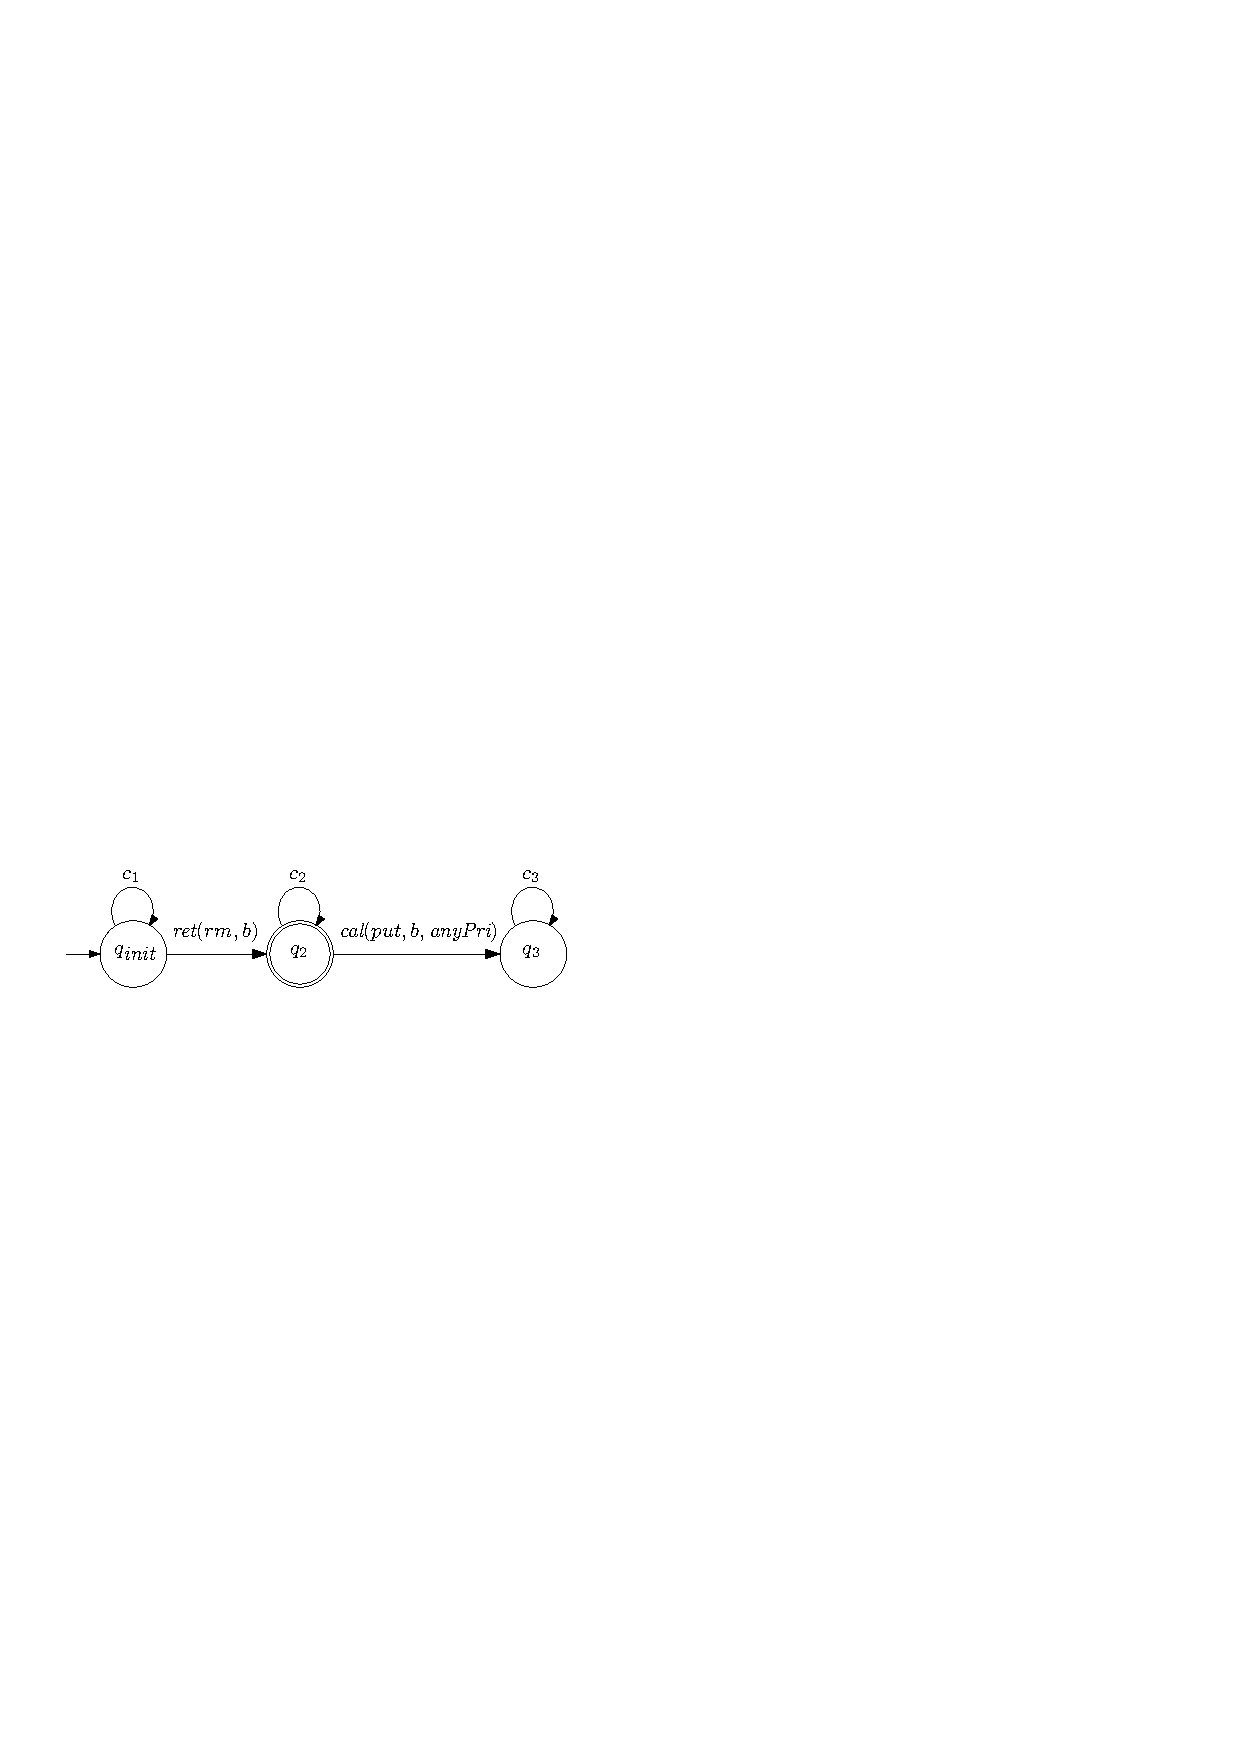
\includegraphics[width=0.5 \textwidth]{PIC_AUTO_UNMATCHED_RM1.pdf}
%\vspace{-10pt}
  \caption{Automaton $\mathcal{A}_{\textit{unmRm1}}$}
  \label{fig:automata for unmatched rm1}
\end{figure}

An automaton $\mathcal{A}_{\textit{unmRm2}}$ is given in \figurename~\ref{fig:automata for unmatched rm2}, where $c_1 = \textit{cal}(\textit{put},a,\textit{anyPri}),\textit{cal}(rm),$ $\textit{ret}(\textit{put}),\textit{ret}(\textit{rm},a)$, and $c_1 = c_1 + \textit{ret}(\textit{rm},b)$.  $\mathcal{A}_{\textit{unmRm1}}$ is used to detect the existence of a item that has been removed more than once but has been inserted once.

\begin{figure}[htbp]
  \centering
  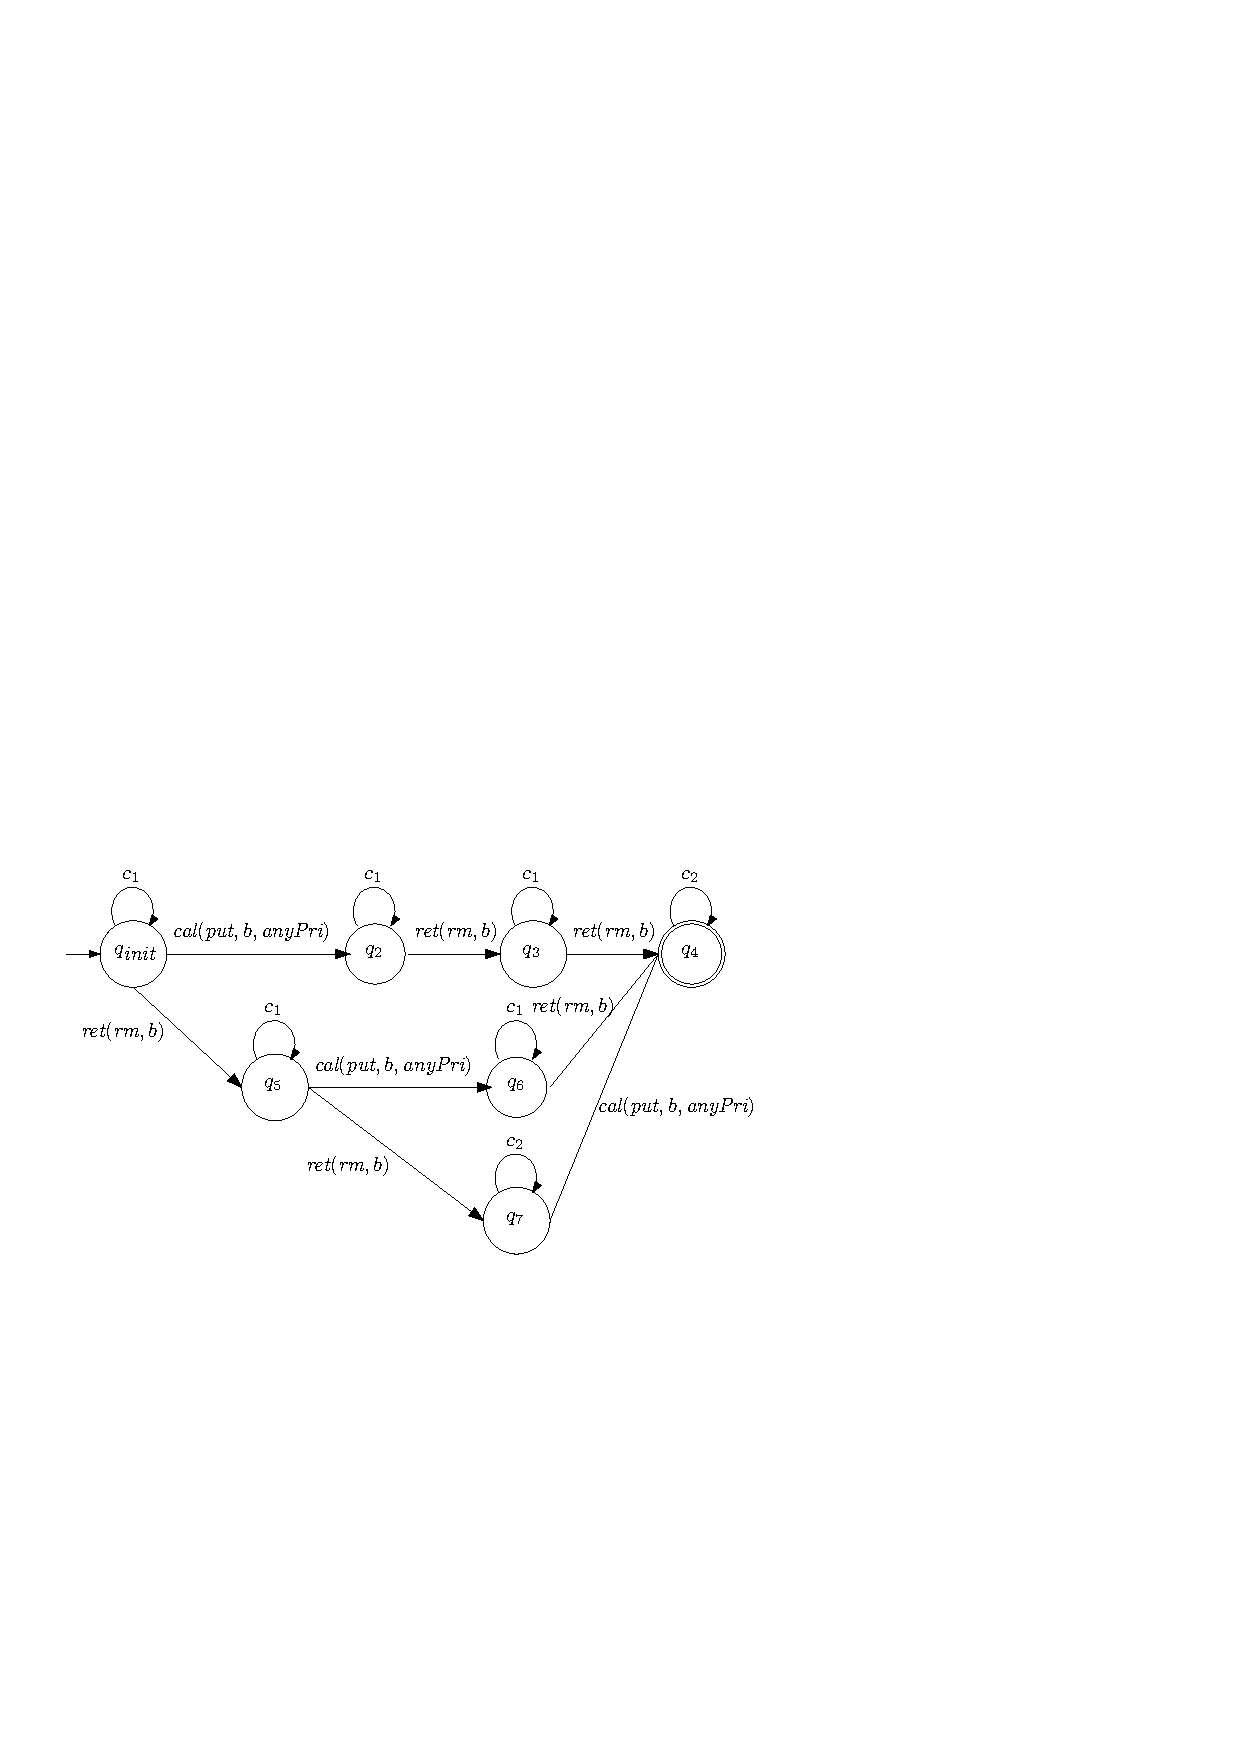
\includegraphics[width=0.5 \textwidth]{PIC_AUTO_UNMATCHED_RM2.pdf}
%\vspace{-10pt}
  \caption{Automaton $\mathcal{A}_{\textit{unmRm2}}$}
  \label{fig:automata for unmatched rm2}
\end{figure}



The following lemma states that we can detect the existence of unmatched $\textit{rm}$ by $\mathcal{A}_{\textit{unmRm1}}$ and $\mathcal{A}_{\textit{unmRm2}}$.

\begin{restatable}{lemma}{DetectUnmatchedRmByAutomata}
\label{lemma:detect unmatched rm by automata}

Given a data-independent $\mathcal{I}$, there is some unmatched $\textit{rm}$ in some sequence of $\mathcal{I}$, if and only if $( \mathcal{I} \cap \mathcal{A}_{\textit{unmRm1}} \neq \emptyset) \vee ( \mathcal{I} \cap \mathcal{A}_{\textit{unmRm2}} \neq \emptyset )$.
\end{restatable}

\begin {proof}

For the $\textit{if}$ direction, assume that $( \mathcal{I} \cap \mathcal{A}_{\textit{unmRm1}} \neq \emptyset) \vee ( \mathcal{I} \cap \mathcal{A}_{\textit{unmRm2}} \neq \emptyset )$. Then, there exists a sequence $l \in \mathcal{I}$ and $l$ is accepted by $\mathcal{A}_{\textit{unmRm1}}$ or $\mathcal{A}_{\textit{unmRm2}}$. If $l$ is accepted by $\mathcal{A}_{\textit{unmRm1}}$, then $l$ contains at least one $\textit{rm}(b)$ operation and no $\textit{put}(b,\_)$ operation; Else, if $l$ is accepted by $\mathcal{A}_{\textit{unmRm2}}$, then $l$ contains at least two $\textit{rm}(b)$ operations and one $\textit{put}(b,\_)$ operation. In both cases, $l$ contains unmatched $\textit{rm}$ operations.

To prove the $\textit{only if}$ direction assume that there exists a sequence $l \in \mathcal{I}$ that contains unmatched $\textit{rm}$ operations. By data-independence, there exists data-differentiated sequence $l'$ and renaming function $r$, such that $l=r(l')$. We need to prove that in $l'$, one of the following cases holds: (1) $l'$ contains $\textit{rm}(d_1)$ for some $d_1$ and does not contain any $\textit{put}(d_1,\_)$, and (2) $l'$ contains one $\textit{put}(d_1,\_)$ operation and more than one $\textit{rm}(d_1)$ operations. We prove this by contradiction. Assume by contradiction that both cases do not hold. Then, for each value $d$ of $l'$, there is either one $\textit{put}(d,\_)$ and one $\textit{rm}(d)$ in $l'$, or one $\textit{put}(d,\_)$ and no $\textit{rm}(d)$ in $l'$. It is obvious that such $l'$ does not contain unmatched $\textit{rm}$ operation, and renaming a sequence that does not contain unmatched $\textit{rm}$ we can only obtain another sequence that does not contain unmatched $\textit{rm}$. This contradicts that $l=r(l')$ has unmatched $\textit{rm}$.

Let $l''$ be obtained from $ll$ by renaming $d_1$ to $b$ and renaming other value to $a$. If the first case holds, $l''$ is accepted by $\mathcal{A}_{\textit{unmRm1}}$; Otherwise, the second case holds, and $l''$ is accepted by $\mathcal{A}_{\textit{unmRm2}}$. \qed
\end {proof}

Therefore, from now on, we can safely assume that there are no unmatched $\textit{rm}$ operations.











































\section{Co-Regular of Priority Queues}
\label{sec:co-regular of priority queues}




\subsection{Co-Regular of $R_{\textit{pr1}}$}
\label{subsec:co-regular of Rpr1}

Let us introduce the notion of gap for matched $\textit{put}$ and $\textit{rm}$ operations.

\begin{definition}[gap for matched $\textit{put}$ and $\textit{rm}$ operations]\label{def:gap for matched put and rm operations}

Let $h$ be a data-differentiated history and $o_1 = \textit{put}(x,\textit{pri}_x)$, $o_2 = \textit{rm}(x)$ be a pair of matched $\textit{put}$ and $\textit{rm}$ operation of $h$. We say that $h$ has a gap on operations $o_1$ and $o_2$, if there is a partition of the operations of $h$ into $L$, $M$ and $R$ satisfying:
\begin{itemize}
\setlength{\itemsep}{0.5pt}
\item[-] $L \cup M$ has matched $\textit{put}$ and $\textit{rm}$ operations.

\item[-] no operation of $R$ happens before an operation of $L$, $o_1$, $M$ or $o_2$.

\item[-] no operation of $o_2$ happens before an operation of $L$, $o_1$ or $M$.

\item[-] no operation of $M$ happens before an operation of $L$ or $o_1$.

\item[-] no operation of $o_1$ happens before an operation of $L$.

\item[-] no operation in $L \cup M \cup R$ has priority $\textit{pri}_x$.
\end{itemize}
\end{definition}

Given a history $h$ and set $O$ of some operations in $h$. It is easy to see that there exists a sequence $l$ of operations of $O$, such that $l$ does not contradicts the happen before relation of $h$. Therefore, from now on, we can use this fact to directly generate such sequence from such $O$.


The following lemma reduce linearizable with respect to $\textit{MR}_{\textit{pr1}}$ into gap of matched $\textit{put}$ and $\textit{rm}$ operations.

\begin{restatable}{lemma}{GapEqualsLinforRpr1}
\label{lemma:Gap Equals Lin for Rpr1}
A data-differentiated history $h$ has a projection $h'$, such that $\textit{last}(h') = R_{\textit{pr1}}$ and $h'$ does not linearizable to $\textit{MR}_{\textit{pr1}}$, if and only if there exists a projection $h''$ of $h$, such that $\textit{last}(h'') = R_{\textit{pr1}}$, $\textit{put}(x,\textit{pri}_x)$ and $\textit{rm}(x)$ is in $h''$, $\textit{pri}_x$ is the maximal priority of $h''$, and one the the following case holds:

\begin{itemize}
\setlength{\itemsep}{0.5pt}
\item[-] case $1$: $\textit{rm}(x)$ happens before $\textit{put}(x,\textit{pri}_x)$,
\item[-] case $2$: there is no gap on $\textit{put}(x,\textit{pri}_x)$ and $\textit{rm}(x)$.
\end{itemize}
\end{restatable}

\begin {proof}

Let us prove the $\textit{only if}$ direction by contradiction. Assume that there exists such $h'$, while case $1$ and case $2$ do not hold for any projection of $h$. Since case $1$ does not hold for any projection of $h$, we know that $\forall y \in D$, $\textit{rm}(y)$ does not happens before $\textit{put}(y,\_)$ in $h$. Since case $2$ does not hold for any projection of $h$ and $\textit{last}(h') = R_{\textit{pr1}}$, we can see that $h'$ has gap on $\textit{put}(x,\textit{pri}_x)$ and $\textit{rm}(x)$, while $\textit{pri}_x$ is the maximal priority in $h'$. Since $\textit{last}(h') = R_{\textit{pr1}}$, we can see that $\textit{pri}_x$ is larger than priority of all other $\textit{put}$ operations of $h$.

By the properties of the gap, there is partitions $L$, $M$ and $R$. Let $u$, $v$ and $w$ contain the operations of $L$, $M$ and $R$, respectively. It is easy to see that $h'$ is linearizable with respect to $l''=u \cdot \textit{put}(x,\textit{pri}) \cdot v \cdot \textit{rm}(x) \cdot w$ and $l'' \in \textit{MR}_{\textit{pr1}}$. This contradicts the fact that $h'$ does not linearizable to $\textit{MR}_{\textit{pr1}}$.

Let us begin to prove the $\textit{if}$ direction.

\begin{itemize}
\setlength{\itemsep}{0.5pt}
\item[-] If case $1$ holds for $h''$, then $h \vert_{ \{ x \} }$ is the $h'$ as required.

\item[-] If case $2$ holds, assume by contradiction that, for every projection $h'$ of $h$, if $\textit{last}(h') = R_{\textit{pr1}}$, then $h' \sqsubseteq \textit{MR}_{\textit{pr1}}$. Since $h''$ is also a projection of $h$, we know that there exist sequences $u$, $v$ and $w$, such that $h'' \sqsubseteq u \cdot \textit{put}(x,\textit{pri}_x) \cdot v \cdot \textit{rm}(x) \cdot w$, $u \cdot v$ contains matched $\textit{put}$ and $\textit{rm}$ operations, and $\textit{pri}_x$ is larger than priority of $u \cdot v \cdot w$. Let $L$, $M$ and $R$ be the operations of $u$, $v$ and $w$, respectively. Then, the partitions $L$, $M$ and $R$ form a gap on operation $\textit{put}(x,\textit{pri}_x)$ and $\textit{rm}(x)$. This contradicts the fact that there is no gap on $\textit{put}(x,\textit{pri}_x)$ and $\textit{rm}(x)$.
\end{itemize}

This completes the proof of this lemma. \qed
\end {proof}

\begin{definition}[left-right constraint for matched $\textit{put}$ and $\textit{rm}$ operations]\label{def:left-right constraint for matched put and rm operations}
Given a data-differentiated history $h$, and two operations $\textit{put}(x,\textit{pri}_x)$ and $\textit{rm}(x)$ of $h$. The left-right constraint of $\textit{put}(x,\textit{pri}_x)$ and $\textit{rm}(x)$ is the graph $G$ where:

\begin{itemize}
\setlength{\itemsep}{0.5pt}
\item[-] the nodes are the items of $h$, to which we add a node,

\item[-] there is an edge from item $d_1$ to $x$, if $\textit{put}(d_1,\textit{pri}_1)$ happens before $\textit{put}(x,\textit{pri}_x)$ or $\textit{rm}(x)$ and $\textit{pri}_1 \neq \textit{pri}_x$,

\item[-] there is an edge from $x$ to item $d_1$, if $\textit{rm}(x)$ happens before $\textit{rm}(d_1)$ or $\textit{rm}(d_1)$ does not exists in $h$, and the priority of $d_1$ is not $\textit{pri}_x$,

\item[-] there is an edge from item $d_1$ to item $d_2$, if $\textit{put}(d_1,\textit{pri}_1)$ happens before $\textit{rm}(d_2,\textit{pri}_2)$, $\textit{pri}_1 \neq \textit{pri}_x$, and $\textit{pri}_2 \neq \textit{pri}_x$.
\end{itemize}
\end{definition}

Given a data-differentiated history $h$ and two operations $\textit{put}(x,\textit{pri}_x)$ and $\textit{rm}(x)$ of $h$. Let $\textit{LMSet}_1(h,x) = \{ o \vert$ $o$ is not an operation of $x$, the priority of $o$ does not equal the priority of $x$, and either it happens before $\textit{put}(x)$ or $\textit{rm}(x)$ in $h$, or there is an operation $o'$ with the same item of $o$, such that $o'$ happens before $\textit{put}(x)$ or $\textit{rm}(x)$ in $h$ $\}$. For each $i \geq 1$, let $\textit{LMSet}_{\textit{i+1}}(h,x) = \{ o \vert$ $o$ is not an operation of $x$ or items in $\textit{LMSet}_k(h,x)$ for each $k \leq i$, the priority of $o$ does not equal the priority of $x$, and either it happens before some operation $o' \in \textit{LMSet}_i(h,x)$ in $h$, or there is an operation $o''$ with the same item of $o$ and $o''$ happens before some operation $o' \in \textit{LMSet}_i(h,x)$ in $h$ $\}$. %We can see that for each $i$, $\textit{LMSet}_i(h,x)$ contains matched $\textit{put}$ and $\textit{rm}$ operations, and
We can see that $\textit{LMSet}_i(h,x) \cap \textit{LMSet}_j(h,x) = \emptyset$ for any $i \neq j$. Let $\textit{LMSet}(h,x) = \textit{LMSet}_1(h,x) \cup \textit{LMSet}_2(h,x) \cup \ldots$. %{\color {red} We say that a history $h$ of priority queue is matched before $x$, if (1) $h$ contains no $\textit{rmEmpty}$ operations, (2) $ h \sqsubseteq l_1 \cdot \textit{put}(x,\_) \cdot l_2 \cdot \textit{rm}(x) \cdot l_3$ for some $l_1,l_2,l_3$, and $l_1 \cdot l_2$ contains matched $\textit{put}$ and $\textit{rm}$ operations.}

The following is an example that shows that, given a data-differentiated history $h$, the set $\textit{LMSet}_i(h,x)$ can be non-empty for each $1 \leq i \leq 3$. In \figurename~\ref{fig:his nobound of LMSet} , $\textit{LMSet}_1(h,x) = \{ \textit{put}(a,1),\textit{rm}(a) \}$, $\textit{LMSet}_2(h,x) = \{ \textit{put}(b,1),\textit{rm}(b) \}$ and $\textit{LMSet}_3(h,x) = \{ \textit{put}(a,c),\textit{rm}(c) \}$.

\begin{figure}[htbp]
  \centering
  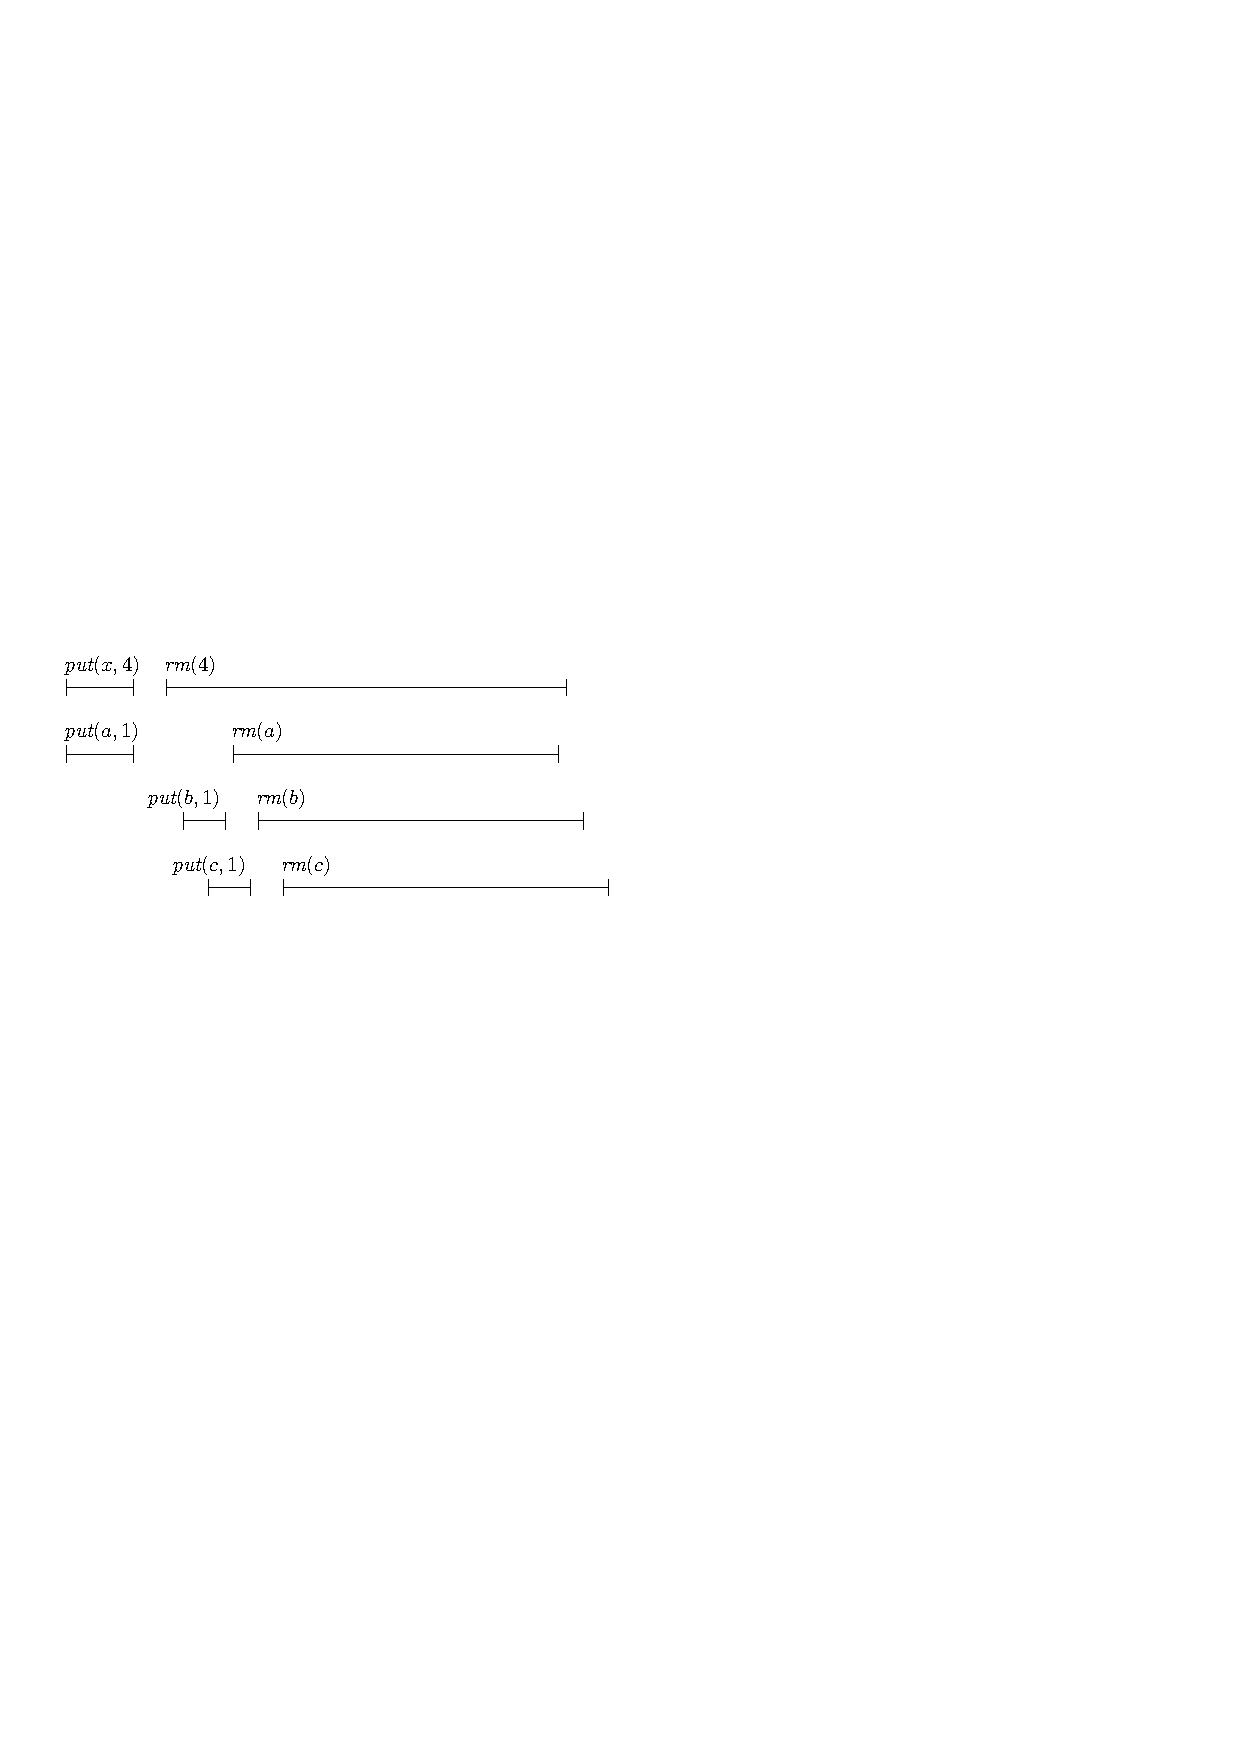
\includegraphics[width=0.5 \textwidth]{PIC_HIS_NOBOUNDOF_LMSET.pdf}
%\vspace{-10pt}
  \caption{An example for non-emptiness of $\textit{LMSet}_1(h,x)$, $\textit{LMSet}_2(h,x)$ and $\textit{LMSet}_3(h,x)$}
  \label{fig:his nobound of LMSet}
\end{figure}


\begin{restatable}{lemma}{RmxDoesNotHappenBeforeLMSetForRpr1}
\label{lemma:Rmx does not happen before LMSet for Rpr1}
Given a data-differentiated history $h$ and two operations $\textit{put}(x,\textit{pri}_x)$ and $\textit{rm}(x)$ of $h$. %, such that $\textit{pri}_x$ is the maximal priority of $h$, and $\textit{last}(h) = R_{\textit{pr1}}$.
Assume that $\textit{rm}(y)$ does not happen before $\textit{put}(y,\_)$ for each item $y$ in $h$. Let $G$ be the graph representing the left-right constraint of $\textit{put}(x,\textit{pri}_x)$ and $\textit{rm}(x)$. Assume that $G$ has no cycle going through $x$. Then, $\textit{rm}(x)$ does not happen before any operation in $\textit{LMSet}(h,x)$.
\end{restatable}

\begin {proof}

We prove this lemma by induction, and prove that $\textit{rm}(x)$ does not happen before any operation in $\textit{LMSet}_1(h,x)$, in $\textit{LMSet}_2(h,x)$, $\ldots$. Note that, according to the definition of $\textit{LMSet}(h,x)$, $\textit{pri}_x$ is different to priority of all items in $\textit{LMSet}(h,x)$.

\noindent (1) Let us prove that $\textit{rm}(x)$ does not happen before any operation in $\textit{LMSet}_1(h,x)$ by contradiction. Assume that $\textit{rm}(x) <_{hb} o$, where $o \in \textit{LMSet}_1(h,x)$ is an operation of item $d$ (according to the definition of $\textit{LMSet}_1(h,x)$, the priority of $d$ does not equals $\textit{pri}_x$).

We use a triple $(t_1,t_2,t_3)$ to represent related information. $t_1,t_2,t_3$ are chosen from $\{ \textit{put},\textit{rm} \}$. $t_1$ represents whether $o$ is a $\textit{put}$ operation or a $\textit{rm}$ operation. $t_2$ and $t_3$ is used for the reason of $o \in \textit{LMSet}_1(h,x)$: $o \in \textit{LMSet}_1(h,x)$, since an operation (of kind $t_2$) of $d$ happens before an operation (of kind $t_3$) of $x$. Let us consider all the possible cases of $(t_1,t_2,t_3)$:

\begin{itemize}
\setlength{\itemsep}{0.5pt}
\item[-] $(\textit{put},\textit{put},\textit{put})$: Then $\textit{rm}(x) <_{hb} \textit{put}(d,\_) <_{hb} \textit{put}(x,\textit{pri}_x)$, contradicts that $\textit{rm}(x)$ does not happen before $\textit{put}(x,\textit{pri}_x)$.

\item[-] $(\textit{put},\textit{put},\textit{rm})$: Then $\textit{rm}(x) <_{hb} \textit{put}(d,\_) <_{hb} \textit{rm}(x)$, contradicts that $\textit{rm}(x)$ does not happen before $\textit{rm}(x)$.

\item[-] $(\textit{put},\textit{rm},\textit{put})$: Then $( \textit{rm}(x) <_{hb} \textit{put}(d,\_) ) \wedge ( \textit{rm}(d) <_{hb} \textit{put}(x,\textit{pri}_x) )$. By interval order, we know that $( \textit{rm}(x) <_{hb} \textit{put}(x,\textit{pri}_x) ) \vee ( \textit{rm}(d) <_{hb} \textit{put}(d,\_) )$, which is impossible.

\item[-] $(\textit{put},\textit{rm},\textit{rm})$: Then $( \textit{rm}(x) <_{hb} \textit{put}(d,\_) ) \wedge ( \textit{rm}(d) <_{hb} \textit{rm}(x) )$. We can see that $\textit{rm}(d) <_{hb} \textit{rm}(x) <_{hb} \textit{put}(d,\_)$, which contradicts that $\textit{rm}(d)$ does not happen before $\textit{put}(d,\_)$.

\item[-] $(\textit{rm},\textit{put},\textit{put})$: Then $( \textit{rm}(x) <_{hb} \textit{rm}(d) ) \wedge ( \textit{put}(d,\_) <_{hb} \textit{put}(x,\textit{pri}_x) )$. We can see that $x$ and $d$ has circle in $G$, contradicts that $G$ has no cycle going through $x$.

\item[-] $(\textit{rm},\textit{put},\textit{rm})$: Then $( \textit{rm}(x) <_{hb} \textit{rm}(d) ) \wedge ( \textit{put}(d,\_) <_{hb} \textit{rm}(x) )$. We can see that $x$ and $d$ has circle in $G$, contradicts that $G$ has no cycle going through $x$.

\item[-] $(\textit{rm},\textit{rm},\textit{put})$: Then $\textit{rm}(x) <_{hb} \textit{rm}(d) <_{hb} \textit{put}(x,\textit{pri}_x)$, contradicts that $\textit{rm}(x)$ does not happen before $\textit{put}(x,\textit{pri}_x)$.

\item[-] $(\textit{rm},\textit{rm},\textit{rm})$: Then $\textit{rm}(x) <_{hb} \textit{rm}(d) <_{hb} \textit{rm}(x)$, contradicts that $\textit{rm}(x)$ does not happen before $\textit{rm}(x)$.
\end{itemize}

This completes the proof for $\textit{LMSet}_1(h,x)$.

\noindent (2) Assume we already prove that for some $j \geq 1$, $\textit{rm}(x)$ does not happen before any operation in $\textit{LMSet}_1(h,x) \cup \ldots \cup \textit{LMSet}_j(h,x)$. Let us prove that $\textit{rm}(x)$ does not happen before any operation in $\textit{LMSet}_{\textit{j+1}}(h,x)$ by contradiction. Assume that $\textit{rm}(x) <_{hb} o$, where $o \in \textit{LMSet}_{\textit{j+1}}(h,x)$ is an operation of item $d_{\textit{j+1}}$ (according to the definition of $\textit{LMSet}_1(h,x)$, the priority of $d_{\textit{j+1}}$ does not equals $\textit{pri}_x$). We use a triple $(t_1,t_2,t_3)$ to represent related information. $t_1,t_2,t_3$ are chosen from $\{ \textit{put},\textit{rm} \}$. $t_1$ represents whether $o$ is a $\textit{put}$ operation or a $\textit{rm}$ operation. $t_2$ and $t_3$ is used for the reason of $o \in \textit{LMSet}_{\textit{j+1}}(h,x)$: $o \in \textit{LMSet}_{\textit{j+1}}(h,x)$, since an operation (of kind $t_2$) of $d_{\textit{j+1}}$ happens before an operation (of kind $t_3$) of $d_j$, where $\textit{put}(d_j,\_), \textit{rm}(d_j) \in \textit{LMSet}_j(h,x)$. Let us consider all the possible cases of $(t_1,t_2,t_3)$:

\begin{itemize}
\setlength{\itemsep}{0.5pt}
\item[-] $(\textit{put},\textit{put},\textit{put})$: Then $\textit{rm}(x) <_{hb} \textit{put}(d_{\textit{j+1}},\_) <_{hb} \textit{put}(d_j,\_)$. We can see that $( \textit{rm}(x) <_{hb} \textit{put}(d_j,\_) ) \wedge ( \textit{put}(d_j,\_) \in \textit{LMSet}_j(h,x) )$, which contradicts that $\textit{rm}(x)$ does not happen before any operation in $\textit{LMSet}_1(h,x) \cup \ldots \cup \textit{LMSet}_j(h,x)$.

\item[-] $(\textit{put},\textit{put},\textit{rm})$: Then $\textit{rm}(x) <_{hb} \textit{put}(d_{\textit{j+1}},\_) <_{hb} \textit{rm}(d_j,\_)$. We can see that $( \textit{rm}(x) <_{hb} \textit{rm}(d_j,\_) ) \wedge ( \textit{rm}(d_j) \in \textit{LMSet}_j(h,x) )$, which contradicts that $\textit{rm}(x)$ does not happen before any operation in $\textit{LMSet}_1(h,x) \cup \ldots \cup \textit{LMSet}_j(h,x)$.

\item[-] $(\textit{put},\textit{rm},\textit{put})$: Then $( \textit{rm}(x) <_{hb} \textit{put}(d_{\textit{j+1}},\_) ) \wedge ( \textit{rm}(d_{\textit{j+1}}) <_{hb} \textit{put}(d_j,\_) )$. By interval order, we know that $( \textit{rm}(x) <_{hb} \textit{put}(d_j,\_) ) \vee ( \textit{rm}(d_{\textit{j+1}}) <_{hb} \textit{put}(d_{\textit{j+1}},\_) )$, which is impossible.

\item[-] $(\textit{put},\textit{rm},\textit{rm})$: Then $( \textit{rm}(x) <_{hb} \textit{put}(d_{\textit{j+1}},\_) ) \wedge ( \textit{rm}(d_{\textit{j+1}}) <_{hb} \textit{rm}(d_j) )$. By interval order, we know that $( \textit{rm}(x) <_{hb} \textit{rm}(d_j) ) \vee ( \textit{rm}(d_{\textit{j+1}}) <_{hb} \textit{put}(d_{\textit{j+1}},\_) )$, which is impossible.

\item[-] $(\textit{rm},\textit{put},\textit{put})$: Then $( \textit{rm}(x) <_{hb} \textit{rm}(d_{\textit{j+1}}) ) \wedge ( \textit{put}(d_{\textit{j+1}},\_) <_{hb} \textit{put}(d_j,\_) )$. Let us consider the reason of $\textit{put}(d_j,\_), \textit{rm}(d_j) \in \textit{LMSet}_j(h,x)$:
    \begin{itemize}
    \setlength{\itemsep}{0.5pt}
    \item[-] If $( j > 1 ) \wedge ( \textit{put}(d_j,\_) <_{hb} o'' )$, where $o''$ is an operation of item $d_{\textit{j-1}}$ and $\textit{put}(_{\textit{j-1}},\_), \textit{rm}(_{\textit{j-1}}) \in \textit{LMSet}_{\textit{j-1}}(h,x)$: Then since $( \textit{put}(d_{\textit{j+1}},\_) <_{hb} \textit{put}(d_j,\_) ) \wedge ( \textit{put}(d_j,\_) <_{hb} o'' )$, we can see that $\textit{put}(d_{\textit{j+1}},\_) <_{hb} o''$, and then operations of $d_{\textit{j+1}}$ is in $\textit{LMSet}_j(h,x)$, contradicts that operations of $d_{\textit{j+1}}$ is in $\textit{LMSet}_{\textit{j+1}}(h,x)$.

    \item[-] If $( j = 1 ) \wedge ( \textit{put}(d_j,\_) <_{hb} o'' )$, where $o''$ is an operation of $x$: Similar to above case.

    \item[-] If $( j > 1 ) \wedge ( \textit{rm}(d_j) <_{hb} o'' )$, where $o''$ is an operation of item $d_{\textit{j-1}}$ and $\textit{put}(d_{\textit{j-1}},\_), \textit{rm}(d_{\textit{j-1}}) \in \textit{LMSet}_{\textit{j-1}}(h,x)$: Then since $( \textit{put}(d_{\textit{j+1}},\_) <_{hb} \textit{put}(d_j,\_) ) \wedge ( \textit{rm}(d_j) <_{hb} o'' )$, we can see that $( \textit{put}(d_{\textit{j+1}},\_) <_{hb} o'' ) \vee ( \textit{rm}(d_j) <_{hb} \textit{put}(d_j,\_) )$, which is impossible.

    \item[-] If $( j > 1 ) \wedge ( \textit{rm}(d_j) <_{hb} o'' )$, where $o''$ is an operation of $x$: Similar to above case.
    \end{itemize}

\item[-] $(\textit{rm},\textit{put},\textit{rm})$: Let $T_{\textit{ind}}$ be the set of sentences $\{ \textit{rm}(x) <_{hb} \textit{rm}(d_{\textit{j+1}}), \textit{put}(d_{\textit{j+1}},\_) <_{hb} \textit{rm}(d_j),\ldots, \textit{put}(d_{\textit{ind+1}},\_) <_{hb} \textit{rm}(d_{\textit{ind}}) \}$. Here each $d_i$ is a item of some operation in $\textit{LMSet}_i(h,x)$ (according to the definition of $\textit{LMSet}_1(h,x)$, the priority of $d_i$ does not equals $\textit{pri}_x$ for each $i$). Let us prove that from $T_j$ we can obtain contradiction by induction:

    {\bf Base case $1$}: From $T_1$ we can obtain contradiction.

    Let us prove base case $1$:

    \begin{itemize}
    \setlength{\itemsep}{0.5pt}
    \item[-] If $\textit{put}(d_1,\_)$ happens $o$, and $o$ is an operation of $x$. Then there is a cycle $x \rightarrow d_{\textit{j+1}} \rightarrow \ldots \rightarrow d_1 \rightarrow x$ in $G$, contradicts that $G$ has no cycle going through $x$.

    \item[-] If $\textit{rm}(d_1)$ happens before $o$, and $o$ is an operation of $x$. Then since $\textit{put}(d_2,\_) <_{hb} \textit{rm}(d_1)$ and $\textit{rm}(d_1) <_{hb} o$, we can see that $\textit{put}(d_2,\_) <_{hb} o$, and then $\textit{put}(d_2,\_) \in \textit{LMSet}_1(h,x)$, contradicts that $\textit{put}(d_2,\_) \in \textit{LMSet}_2(h,x)$.
    \end{itemize}

    {\bf Base case $2$}: From $T_2$ we can obtain contradiction.

    Let us prove base case $2$: If $\textit{rm}(d_2) <_{hb} o$, and $o$ is an operation of $d_1$, then since $( \textit{put}(d_3,\_) <_{hb} \textit{rm}(d_2) ) \wedge ( \textit{rm}(d_2) <_{hb} o )$, we know that $\textit{put}(d_3,\_) <_{hb} o$. This implies that $\textit{put}(d_3,\_) \in \textit{LMSet}_2(h,x)$, contradicts that $\textit{rm}(d_3,\_) \in \textit{LMSet}_3(h,x)$. Therefore, it is only possible that $\textit{put}(d_2,\_)$ happens before an operation of $d_1$.

    \begin{itemize}
    \setlength{\itemsep}{0.5pt}
    \item[-] If $\textit{put}(d_2,\_) <_{hb} \textit{put}(d_1,\_)$ and $\textit{put}(d_1,\_)$ happens before operations of $x$, then we know that $\textit{put}(d_2,\_)$ happens before operation of $x$, which is impossible.

    \item[-] If $\textit{put}(d_2,\_) <_{hb} \textit{put}(d_1,\_)$ and $\textit{rm}(d_1)$ happens before operations of $x$, then by interval order, we know that $\textit{put}(d_2,\_)$ happens before operation of $x$, or $\textit{rm}(d_1) <_{hb} \textit{put}(d_1,\_)$, which is impossible.

    \item[-] If $\textit{put}(d_2,\_) <_{hb} \textit{rm}(d_1)$ and $\textit{put}(d_1,\_)$ happens before operations of $x$, then $x \rightarrow d_{\textit{j+1}} \rightarrow \ldots \rightarrow d_1 \rightarrow x$ in $G$, contradicts that $G$ has no cycle going through $x$.

    \item[-] If $\textit{put}(d_2,\_) <_{hb} \textit{rm}(d_1)$ and $\textit{rm}(d_1)$ happens before operations of $x$, then we know that $\textit{put}(d_2,\_)$ happens before operation of $x$, which is impossible.
    \end{itemize}

    {\bf induction step}: Given $\textit{ind} \geq 3$, if from $T_{\textit{ind-1}}$ we can obtain contradiction, then from $T_{\textit{ind}}$ we can also contain contradiction.


    Prove of the induction step: Similarly as base case $2$, we can prove that it is only possible that $\textit{put}(d_{\textit{ind}},\_)$ happens before operations of $d_{\textit{ind-1}}$.

    \begin{itemize}
    \setlength{\itemsep}{0.5pt}
    \item[-] If $\textit{put}(d_{\textit{ind}},\_) <_{hb} \textit{put}(d_{\textit{ind-1}},\_)$ and $\textit{put}(d_{\textit{ind-1}},\_)$ happens before operations of $d_{\textit{ind-2}}$, then we know that $\textit{put}(d_{\textit{ind}})$ happens before operation of $d_{\textit{ind-2}}$, which is impossible.

    \item[-] If $\textit{put}(d_{\textit{ind}},\_) <_{hb} \textit{put}(d_{\textit{ind-1}},\_)$ and $\textit{rm}(d_{\textit{ind-1}})$ happens before operations of $d_{\textit{ind-2}}$, then by interval order, we know that $\textit{put}(d_{\textit{ind}},\_)$ happens before operation of $d_{\textit{ind-2}}$, or $\textit{rm}(d_{\textit{ind-1}}) <_{hb} \textit{put}(d_{\textit{ind-1}},\_)$, which is impossible.

    \item[-] If $\textit{put}(d_{\textit{ind}},\_) <_{hb} \textit{rm}(d_{\textit{ind-1}})$, then we obtain $T_{\textit{ind-1}}$, which already contain contradiction.
    \end{itemize}

    By base case $1$, base case $2$ and the induction step, it is easy to see that $T_j$ contains contradiction.

\item[-] $(\textit{rm},\textit{rm},\textit{put})$: Then $( \textit{rm}(x) <_{hb} \textit{rm}(d_{\textit{j+1}}) ) \wedge ( \textit{rm}(d_{\textit{j+1}}) <_{hb} \textit{put}(d_j,\_) )$. We can see that $( \textit{rm}(x) <_{hb} \textit{put}(d_j,\_) ) \wedge ( \textit{put}(d_j,\_) \in \textit{LMSet}_j(h,x) )$, which contradicts that $\textit{rm}(x)$ does not happen before any operation in $\textit{LMSet}_1(h,x) \cup \ldots \cup \textit{LMSet}_j(h,x)$.

\item[-] $(\textit{rm},\textit{rm},\textit{rm})$: Then $( \textit{rm}(x) <_{hb} \textit{rm}(d_{\textit{j+1}}) ) \wedge ( \textit{rm}(d_{\textit{j+1}}) <_{hb} \textit{rm}(d_j) )$. We can see that $( \textit{rm}(x) <_{hb} \textit{rm}(d_j) ) \wedge ( \textit{rm}(d_j) \in \textit{LMSet}_j(h,x) )$, which contradicts that $\textit{rm}(x)$ does not happen before any operation in $\textit{LMSet}_1(h,x) \cup \ldots \cup \textit{LMSet}_j(h,x)$.
\end{itemize}

This completes the proof for $\textit{LMSet}_{\textit{j+1}}(h,x)$. Therefore, $\textit{rm}(x)$ does not happen before any operation in $\textit{LMSet}(h,x) = \textit{LMSet}_1(h,x) \cup \textit{LMSet}_2(h,x) \cup \ldots$. \qed
\end {proof}


\begin{restatable}{lemma}{LMSetHasMatchedPutandRmOperations}
\label{lemma:LMSet has matched put and rm operations}
Given a data-differentiated history $h$ and two operations $\textit{put}(x,\textit{pri}_x)$ and $\textit{rm}(x)$ of $h$. Assume that $\textit{rm}(y)$ does not happen before $\textit{put}(y,\_)$ for each item $y$ in $h$. Let $G$ be the graph representing the left-right constraint of $\textit{put}(x,\textit{pri}_x)$ and $\textit{rm}(x)$. Assume that $G$ has no cycle going through $x$. Then, $\textit{LMSet}(h,x)$ contains only matched $\textit{put}$ and $\textit{rm}$ operations.
\end{restatable}
\begin {proof}

We prove this lemma by contradiction. Assume that there exists a value, such that $\textit{LMSet}(h,x)$ contains only its $\textit{put}$ operation and does not contain its $\textit{rm}$ operation. Then we can see that there exists $d_1,\ldots,d_j$. Intuitively, $d_1,\ldots,d_j$ are items in $\textit{LMSet}_1(h,x), \ldots, \textit{LMSet}_i(h,x)$, respectively. $\textit{LMSet}(h,x)$ contains $\textit{put}(d_j,\_)$ and does not contain $\textit{rm}(d_j)$. And each $d_i$ is the reason of $d_{\textit{i+1}} \in \textit{LMSet}_{\textit{i+1}}(h,x)$. Formally, we require that

\begin{itemize}
\setlength{\itemsep}{0.5pt}
\item[-] For each $1 \leq i \leq j$, operations of $d_i$ belongs to $\textit{LMSet}_i(h,x)$. %For each $1 \leq i \leq j$, the priority of $d_i$ is not $\textit{pri}_x$.

\item[-] For each $i \neq j$, $\textit{put}(d_i,\_),\textit{rm}(d_i) \in \textit{LMSet}_i(h,x)$. $\textit{put}(d_j,\_) \in \textit{LMSet}_j(h,x)$, and $h$ does not contain $\textit{rm}(d_j)$.

\item[-] An operation of $d_1$ happens before an operation of $x$. For each $1 < i \leq j$, an operation of $d_j$ happens an operation of $d_{\textit{i-1}}$.

\item[-] For each $k$ and $\textit{ind}$, if $k > \textit{ind+1}$, then no operation of $d_k$ happens before operation of $d_{\textit{ind}}$.
\end{itemize}

According to the definition of $\textit{LMSet}(h,x)$, it is easy to see that such $d_1,\ldots,d_j$ exists. Let us prove the following fact:

\noindent {\bf $\textit{fact}_1$}: Given $1 \leq i < j$, it can not be the case that $\textit{put}(d_i,\_)$ and $\textit{rm}(d_i)$ overlap.

Proof of $\textit{fact}_1$: We prove $\textit{fact}_1$ by contradiction. Assume that for some $i \neq j$, $\textit{put}(d_i,\_)$ and $\textit{rm}(d_i)$ overlap. Since $\textit{put}(d_i,\_), \textit{rm}(d_i) \in \textit{LMSet}_i(h,x)$, we know that an operation $o_i$ of $d_i$ happens before operation $o_{\textit{i-1}}$ of $d_{\textit{i-1}}$. Moreover, since $\textit{put}(d_i,\_)$ and $\textit{rm}(d_i)$ overlap, it is not hard to see that the call action of $\textit{put}(d_i,\_)$ and the call action of $\textit{rm}(d_i)$ is before the call action of $o_{\textit{i-1}}$. Since $\textit{put}(d_{\textit{i+1}},\_), \textit{rm}(d_{\textit{i+1}}) \in \textit{LMSet}_{\textit{i+1}}(h,x)$, we know that an operation $o'_{\textit{i+1}}$ of $d_{\textit{i+1}}$ happens before operation $o'_i$ of $d_i$. Then, it is not hard to see that $o'_{\textit{i+1}}$ also happens before $o_{\textit{i-1}}$, which contradicts that For each $k > \textit{ind+1}$, no operation of $d_k$ happens before operation of $d_{\textit{ind}}$.

We already know that an operation of $d_1$ happens before an operation of $x$. By $\textit{fact}_1$, we can ensure that $\textit{put}(d_1,\_)$ happens before an operation of $x$, and then $d_1 \rightarrow x$ in $G$. For each $1 < i < j$, we know that an operation $o_i$ of $d_i$ happens before an operation $o_{\textit{i-1}}$ of $d_{\textit{i-1}}$. By $\textit{fact}_1$, we can ensure that $o_i=\textit{put}(d_i,\_)$ and $o_{\textit{i-1}}=\textit{rm}(d_{\textit{i-1}})$, and then $d_i \rightarrow d_{\textit{i-1}}$ in $G$. Since $h$ contains $\textit{put}(d_j)$ and does not contain $\textit{rm}(d_j)$, we know that $x \rightarrow d_j$ in $G$. Then $G$ has a cycle going through $x$, contradicts that $G$ has no cycle going through $x$. \qed
\end {proof}



\begin{restatable}{lemma}{GapEqualsConstraintforRpr1}
\label{lemma:Gap Equals Constraint for Rpr1}
Given a data-differentiated history $h$ and two operations $\textit{put}(x,\textit{pri}_x)$ and $\textit{rm}(x)$ of $h$. %, where $\textit{pri}_x$ has the maximal priority of $h$, and $\textit{last}(h) = R_{\textit{pr1}}$.
Assume that for each item in $h$, its $\textit{rm}$ operation does not happen before its $\textit{put}$ operation. Let $G$ be the graph representing the left-right constraint of $\textit{put}(x)$ and $\textit{rm}(x)$. There is a gap on $\textit{put}(x)$ and $\textit{rm}(x)$, if and only if $G$ has no cycle going through $x$.
\end{restatable}

\begin {proof}

To prove the $\textit{only if}$ direction, assume that there is a gap on $\textit{put}(x)$ and $\textit{rm}(x)$, and let it be $L$, $M$ and $R$. Assume by contradiction that, there is a cycle $d_1 \rightarrow d_2 \rightarrow \ldots \rightarrow d_m \rightarrow x \rightarrow d_1$ in $G$. It is obvious that the priority of each $d_i$ is not $\textit{pri}_x$. Then our proof proceeds as follows:

According to the definition of left-right constraint, there are two possibilities. The first possibility is that, $\textit{rm}(x)$ happens before $\textit{rm}(d_1)$. It is obvious that $\textit{rm}(d_1) \in R$, and then since $L \cup M$ contains matched $\textit{put}$ and $\textit{rm}$ operations, we know that $\textit{put}(d_1),\textit{rm}(d_1) \in R$. Then,

\begin{itemize}
\setlength{\itemsep}{0.5pt}
\item[-] Since $d_1 \rightarrow d_2$, by definition of $G$, we know that $\textit{put}(d_1)$ happens before $\textit{rm}(d_2)$. Since $\textit{put}(d_1) \in R$ and $L \cup M$ contains matched $\textit{put}$ and $\textit{rm}$ operations, we know that $\textit{put}(d_2),\textit{rm}(d_2) \in R$. Similarly, for each $1 \leq i \leq m$, we know that $\textit{put}(d_i),\textit{rm}(d_i) \in R$.

\item[-] Since $d_m \rightarrow x$,
    \begin{itemize}
    \setlength{\itemsep}{0.5pt}
    \item[-] if $\textit{put}(d_m)$ happens before $\textit{put}(x)$, then we can see that $\textit{put}(d_m) \in L$, which contradicts that $\textit{put}(d_m) \in R$.

    \item[-] if $\textit{put}(d_m)$ happens before $\textit{rm}(x)$, then we can see that $\textit{put}(d_m) \in L \cup M$, which contradicts that $\textit{put}(d_m) \in R$.
    \end{itemize}
\end{itemize}

The second possibility is that, $h$ contains one $\textit{put}(d_1,\_)$ operation and no $\textit{rm}(d_1)$ operation. Note that for each $j > 1$, $h$ contains $\textit{put}(d_j,\_)$ and $\textit{rm}(d_j)$. Since $d_m \rightarrow x$, is is obvious that $\textit{put}(d_m) \in L \cup M$. Since $L \cup M$ contains matched $\textit{put}$ and $\textit{rm}$ operations, we know that $\textit{put}(d_m),\textit{rm}(d_m) \in R$. Then,

\begin{itemize}
\setlength{\itemsep}{0.5pt}
\item[-] Since $d_{\textit{m-1}} \rightarrow d_m$, by definition of $G$, we know that $\textit{put}(d_{\textit{m-1}})$ happens before $\textit{rm}(d_m)$. Since $\textit{rm}(d_m) \in L \cup M$ and $L \cup M$ contains matched $\textit{put}$ and $\textit{rm}$ operations, we know that $\textit{put}(d_{\textit{m-1}}),\textit{rm}(d_{\textit{m-1}}) \in L \cup M$. Similarly, for each $1 < i \leq m$, we know that $\textit{put}(d_i),\textit{rm}(d_i) \in L \cup M$, and $\textit{put}(d_1)\in L \cup M$.

\item[-] Since $d_1 \rightarrow d_2$ in $G$, $\textit{put}(d_1,\_)$ happens before $\textit{rm}(d_2)$. Since $\textit{put}(d_2),\textit{rm}(d_2) \in L \cup M$, we can see that $\textit{put}(d_1) \in L \cup M$. However, there is one $\textit{put}(d_1,\_)$ operation and no $\textit{rm}(d_1)$ operation in $h$, contradicts that $L \cup M$ contains matched $\textit{put}$ and $\textit{rm}$ operations.
\end{itemize}


This completes the proof of the $\textit{only if}$ direction.

To prove the $\textit{if}$ direction, assume that $G$ has no cycle going through $x$. Let $O_L$ be the set of operations that happen before $\textit{put}(x)$ in $h$. It is easy to see that $O_L \subseteq \textit{LMSet}(h,x)$. Let $O_M = \textit{LMSet}(h,x) \setminus O_L$. Let $O_h$ be the set of operations of $h$, and let $O_R = O_h \setminus \textit{LMSet}(h,x)$. Let $L$, $M$ and $R$ be $O_L$, $O_M$ and $O_R$, respectively.

By Lemma \ref{lemma:LMSet has matched put and rm operations}, we can see that $L \cup M$ contains matched $\textit{put}$ and $\textit{rm}$ operations. It remains to prove that $L$, $M$ and $R$ is a gap of $\textit{put}(x)$ and $\textit{rm}(x)$. We prove this by showing that all the following cases are impossible:

\begin{itemize}
\setlength{\itemsep}{0.5pt}
\item[-] Case $1$: Some operation $o_r \in R$ happens before $\textit{rm}(x)$. Then we know that $o_r \in \textit{LMSet}(h,x)$, which contradicts that $o_r \in R$.

\item[-] Case $2$: Some operation $o_r \in R$ happens before some operation $o_{lm} \in L \cup M$. Then we know that $o_r \in \textit{LMSet}(h,x)$, which contradicts that $o_r \in R$.

\item[-] Case $3$: Some operation $o_r \in R$ happens before $\textit{put}(x)$. Then we know that $o_r \in \textit{LMSet}(h,x)$, which contradicts that $o_r \in R$.

\item[-] Case $4$: $\textit{rm}(x)$ happens before some $o_{lm} \in \textit{LMSet}(h,x) = L \cup M$. By Lemma \ref{lemma:Rmx does not happen before LMSet for Rpr1} we know that this is impossible.

\item[-] Case $5$: $\textit{rm}(x)$ happens before $\textit{put}(x)$. This contradicts that for each item in $h$, its $\textit{rm}$ operation does not happen before its $\textit{put}$ operation.

\item[-] Case $6$: Some operation $o_m \in M$ happens before $\textit{put}(x)$. Then we know that $o_m \in L$, which contradicts that $o_m \in M$.

\item[-] Case $7$: Some operation $o_m \in M$ happens before some operation $o_l \in L$. Then we know that $o_m \in L$, which contradicts that $o_m \in M$.

\item[-] Case $8$: $\textit{put}(x)$ happens before some operation $o_l \in L$. This is impossible.
\end{itemize}

This completes the proof of the $\textit{if}$ direction.

\qed
\end {proof}



A automaton $\mathcal{A}_{\textit{Rpr1-1}}$ is given in \figurename~\ref{fig:automata for Rpro-1}, where $c=\textit{cal}(\textit{put},a,\textit{anyPri}),\textit{cal}(rm,a),$ $\textit{ret}(\textit{put}),\textit{ret}(\textit{rm},a)$. $\mathcal{A}_{\textit{Rpr1-1}}$ is used to detect the existence of a item whose $\textit{rm}$ happens before its $\textit{put}$.

\begin{figure}[htbp]
  \centering
  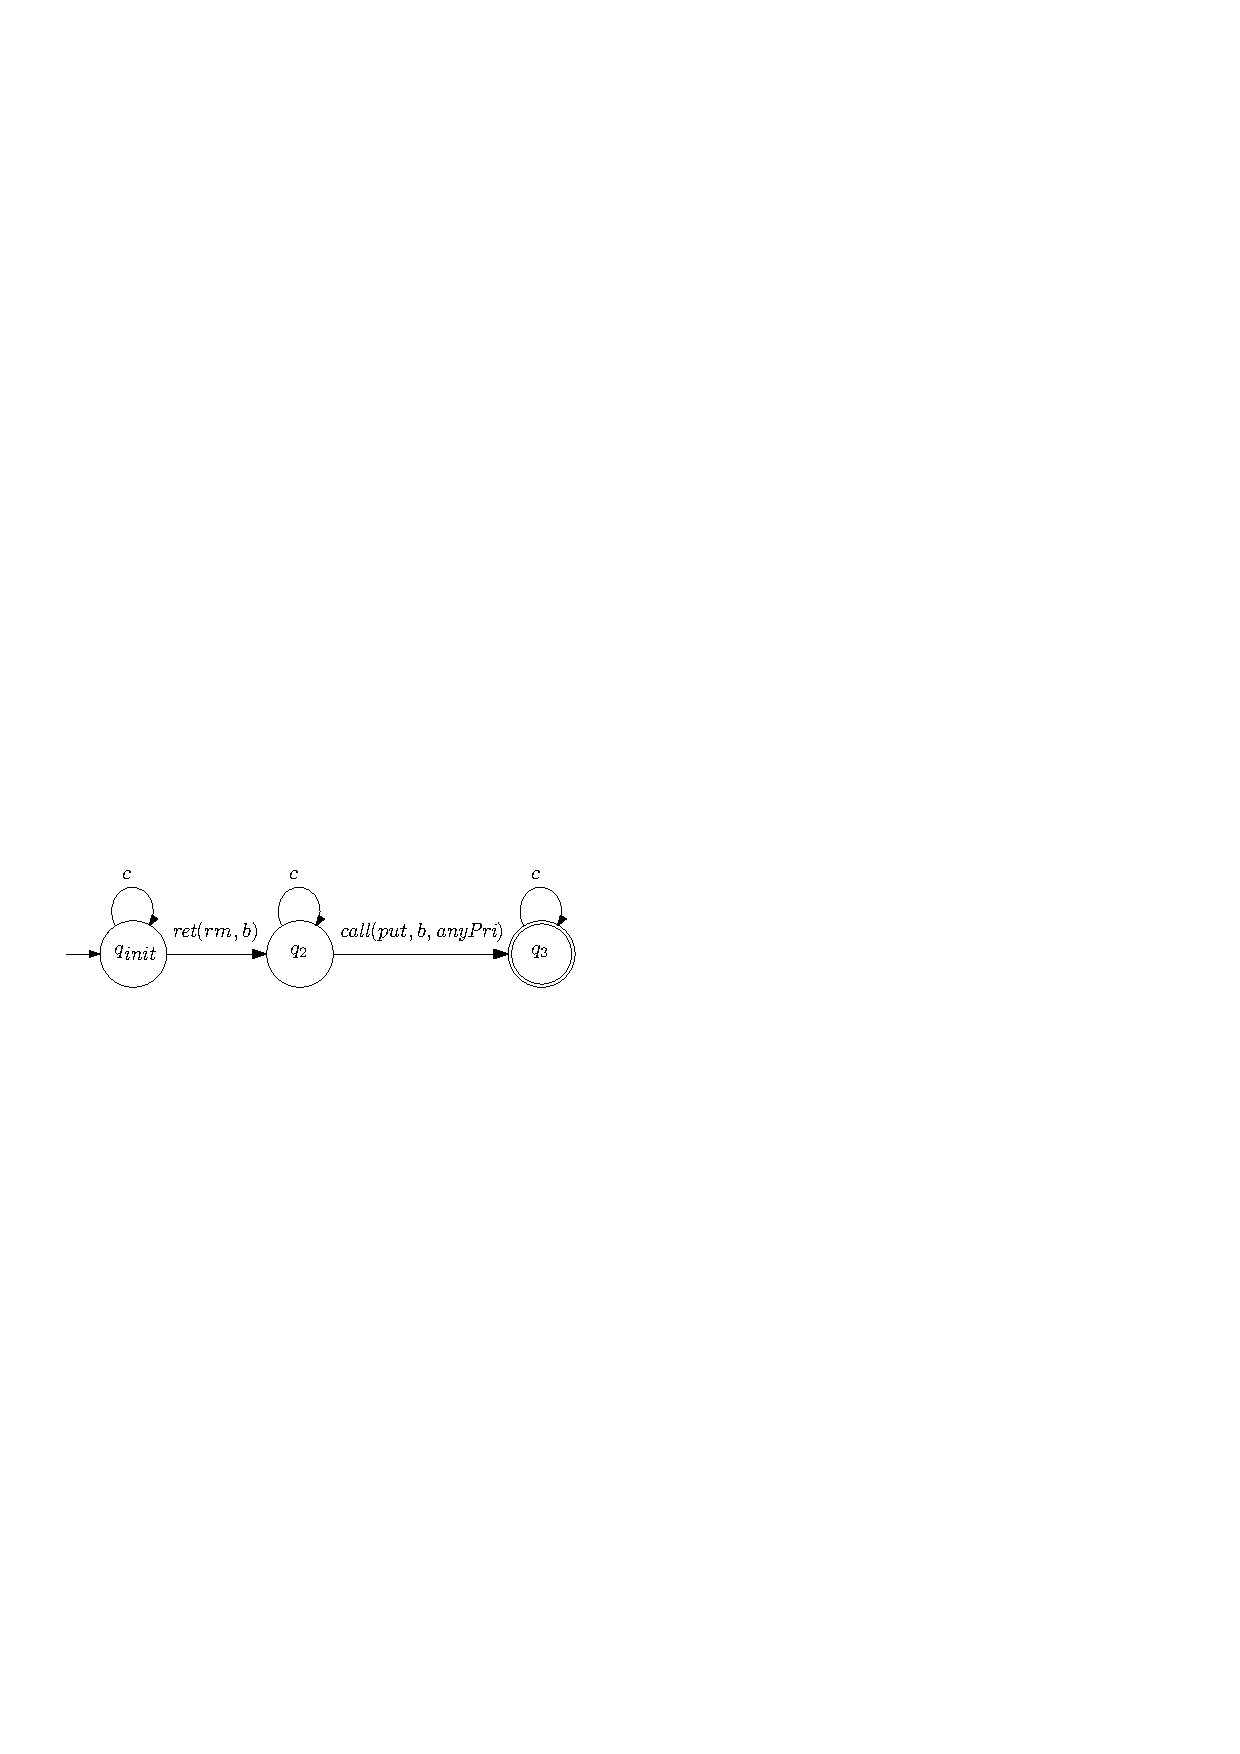
\includegraphics[width=0.5 \textwidth]{PIC_AUTO_UNMATCHED_Rpr1-1.pdf}
%\vspace{-10pt}
  \caption{Automaton $\mathcal{A}_{\textit{Rpr1-1}}$}
  \label{fig:automata for Rpro-1}
\end{figure}

Let us begin to represent several automata that is used for capture the case that, in a sub-history $h'$ of a history $h$, $\textit{last}(h')=R_{\textit{pr1}}$, $h'$ does not linearizable to $\textit{MR}_{\textit{pr1}}$, and the reason is that there is no gap on $\textit{put}(y,\textit{pri}_y)$ and $\textit{rm}(y)$ in $h'$, where $y$ is the item that has maximal priority in $h'$. Such case is dealt with by four automata, since there are four possibilities of $h' \vert_{y}$.

The first automaton is $\mathcal{A}_{\textit{Rpr1-pprr}}$, which is given in \figurename~\ref{fig:automata for Rpro-pprr}. In \figurename~\ref{fig:automata for Rpro-pprr}, $c_1= \textit{cal}(\textit{put},c,$ $\textit{anyPri}),\textit{ret}(\textit{put},c), \textit{cal}(\textit{rm},c), \textit{ret}(\textit{rm},c)$, $c_2 = c_1 + \textit{cal}(\textit{put},a,\textit{les}_p)$, and $c_3 = c_2 + \textit{ret}(\textit{rm},a)$. Here $p$ is a variable for priority, and $\textit{les}_p$ is a predicate that accepts all priorities that are less than the value of $p$. Here $\textit{pprr}$ represents that, $h' \vert_{b} = \textit{cal}(\textit{put},b,p) \cdot \textit{ret}(\textit{put}) \cdot \textit{cal}(\textit{rm}) \cdot \textit{ret}(\textit{rm},b)$ (we consider $b$ as $y$ and $p$ as $\textit{pri}_y$). In \figurename~\ref{fig:automata for Rpro-pprr}, the three paths that (1) from $q_{\textit{init}}$ to $q_2$ to $q_3$, (2) from $q_{\textit{init}}$ to $q_2$ to $q_{11}$, and (3) from $q_{\textit{init}}$ to $q_{10}$ to $q_{11}$ represents three possible positions of $\textit{ret}(\textit{put},a)$.

\begin{figure}[htbp]
  \centering
  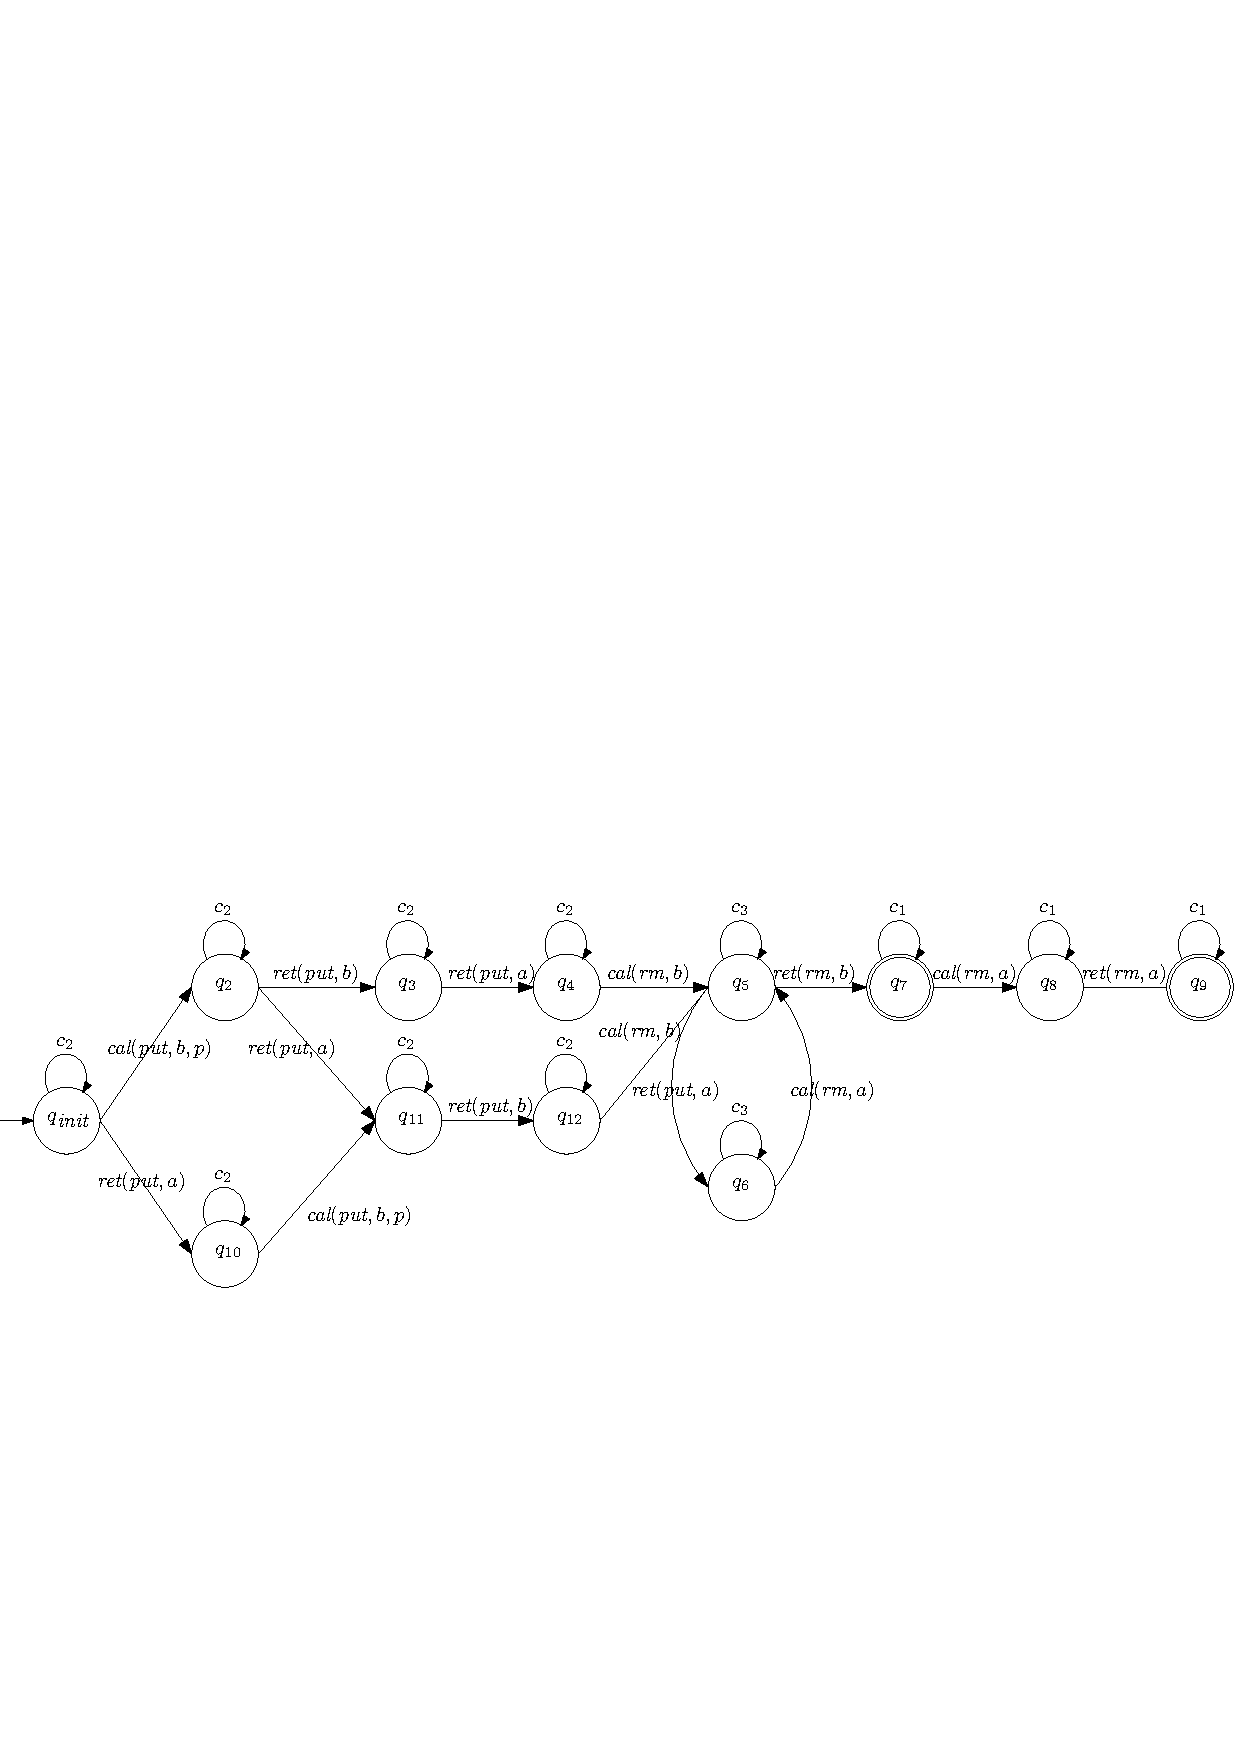
\includegraphics[width=1 \textwidth]{PIC_AUTO_UNMATCHED_Rpr1-pprr.pdf}
%\vspace{-10pt}
  \caption{Automaton $\mathcal{A}_{\textit{Rpr1-pprr}}$}
  \label{fig:automata for Rpro-pprr}
\end{figure}


The second automaton is $\mathcal{A}_{\textit{Rpr1-prpr}}$, which is given in \figurename~\ref{fig:automata for Rpro-prpr}. In $\mathcal{A}_{\textit{Rpr1-prpr}}$, $c_1, c_2, c_3$ is same as that in $\mathcal{A}_{\textit{Rpr1-pprr}}$. Here $\textit{pprr}$ represents that, $h' \vert_{2} = \textit{cal}(\textit{put},b,p) \cdot \textit{cal}(\textit{rm}) \cdot \textit{ret}(\textit{put}) \cdot \textit{ret}(\textit{rm},b)$.

\begin{figure}[htbp]
  \centering
  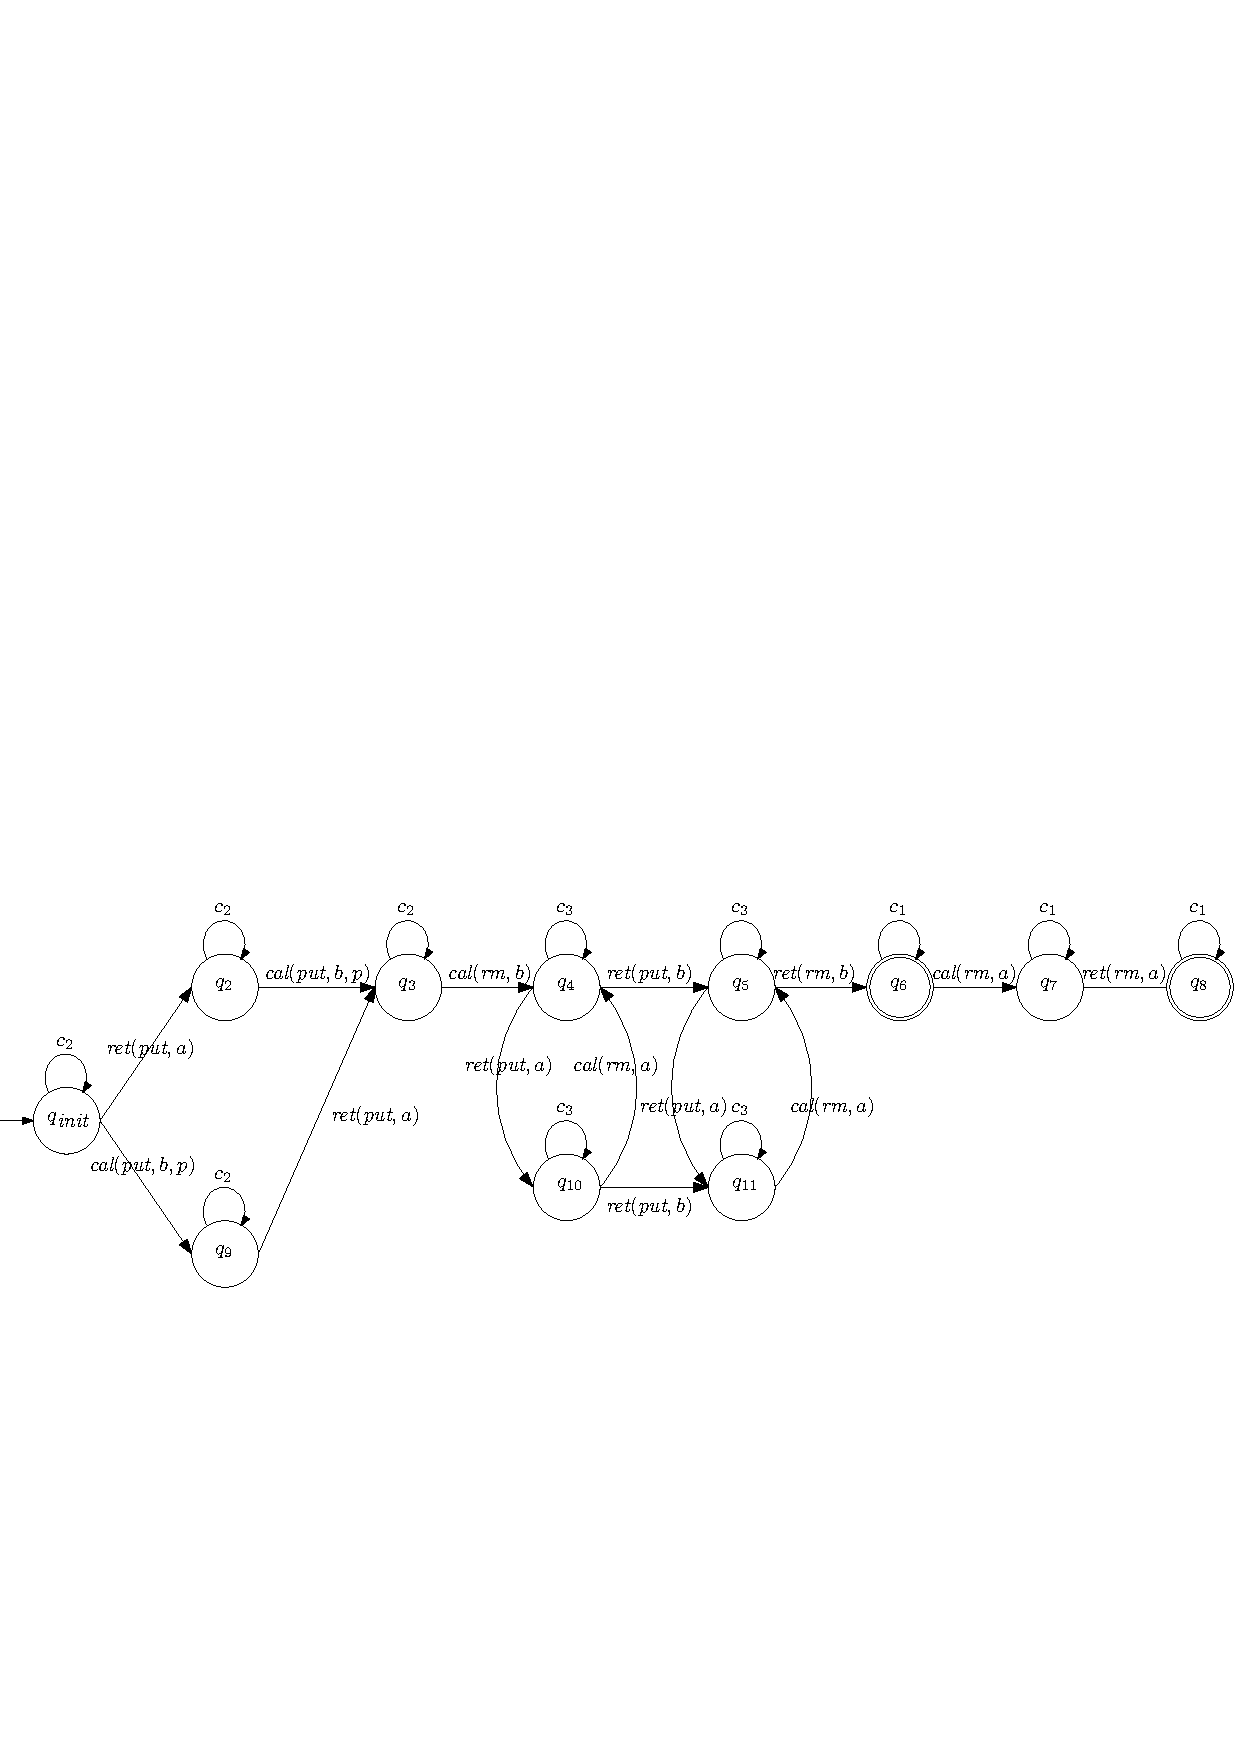
\includegraphics[width=1 \textwidth]{PIC_AUTO_UNMATCHED_Rpr1-prpr.pdf}
%\vspace{-10pt}
  \caption{Automaton $\mathcal{A}_{\textit{Rpr1-prpr}}$}
  \label{fig:automata for Rpro-prpr}
\end{figure}



The third automaton is $\mathcal{A}_{\textit{Rpr1-rppr}}$, which is given in \figurename~\ref{fig:automata for Rpro-rppr}. In $\mathcal{A}_{\textit{Rpr1-rppr}}$, $c_1, c_2, c_3$ is same as that in $\mathcal{A}_{\textit{Rpr1-pprr}}$. Here $\textit{rppr}$ represents that, $h' \vert_{2} = \textit{cal}(\textit{rm}) \cdot \textit{cal}(\textit{put},b,p) \cdot \textit{ret}(\textit{put}) \cdot \textit{ret}(\textit{rm},b)$.

\begin{figure}[htbp]
  \centering
  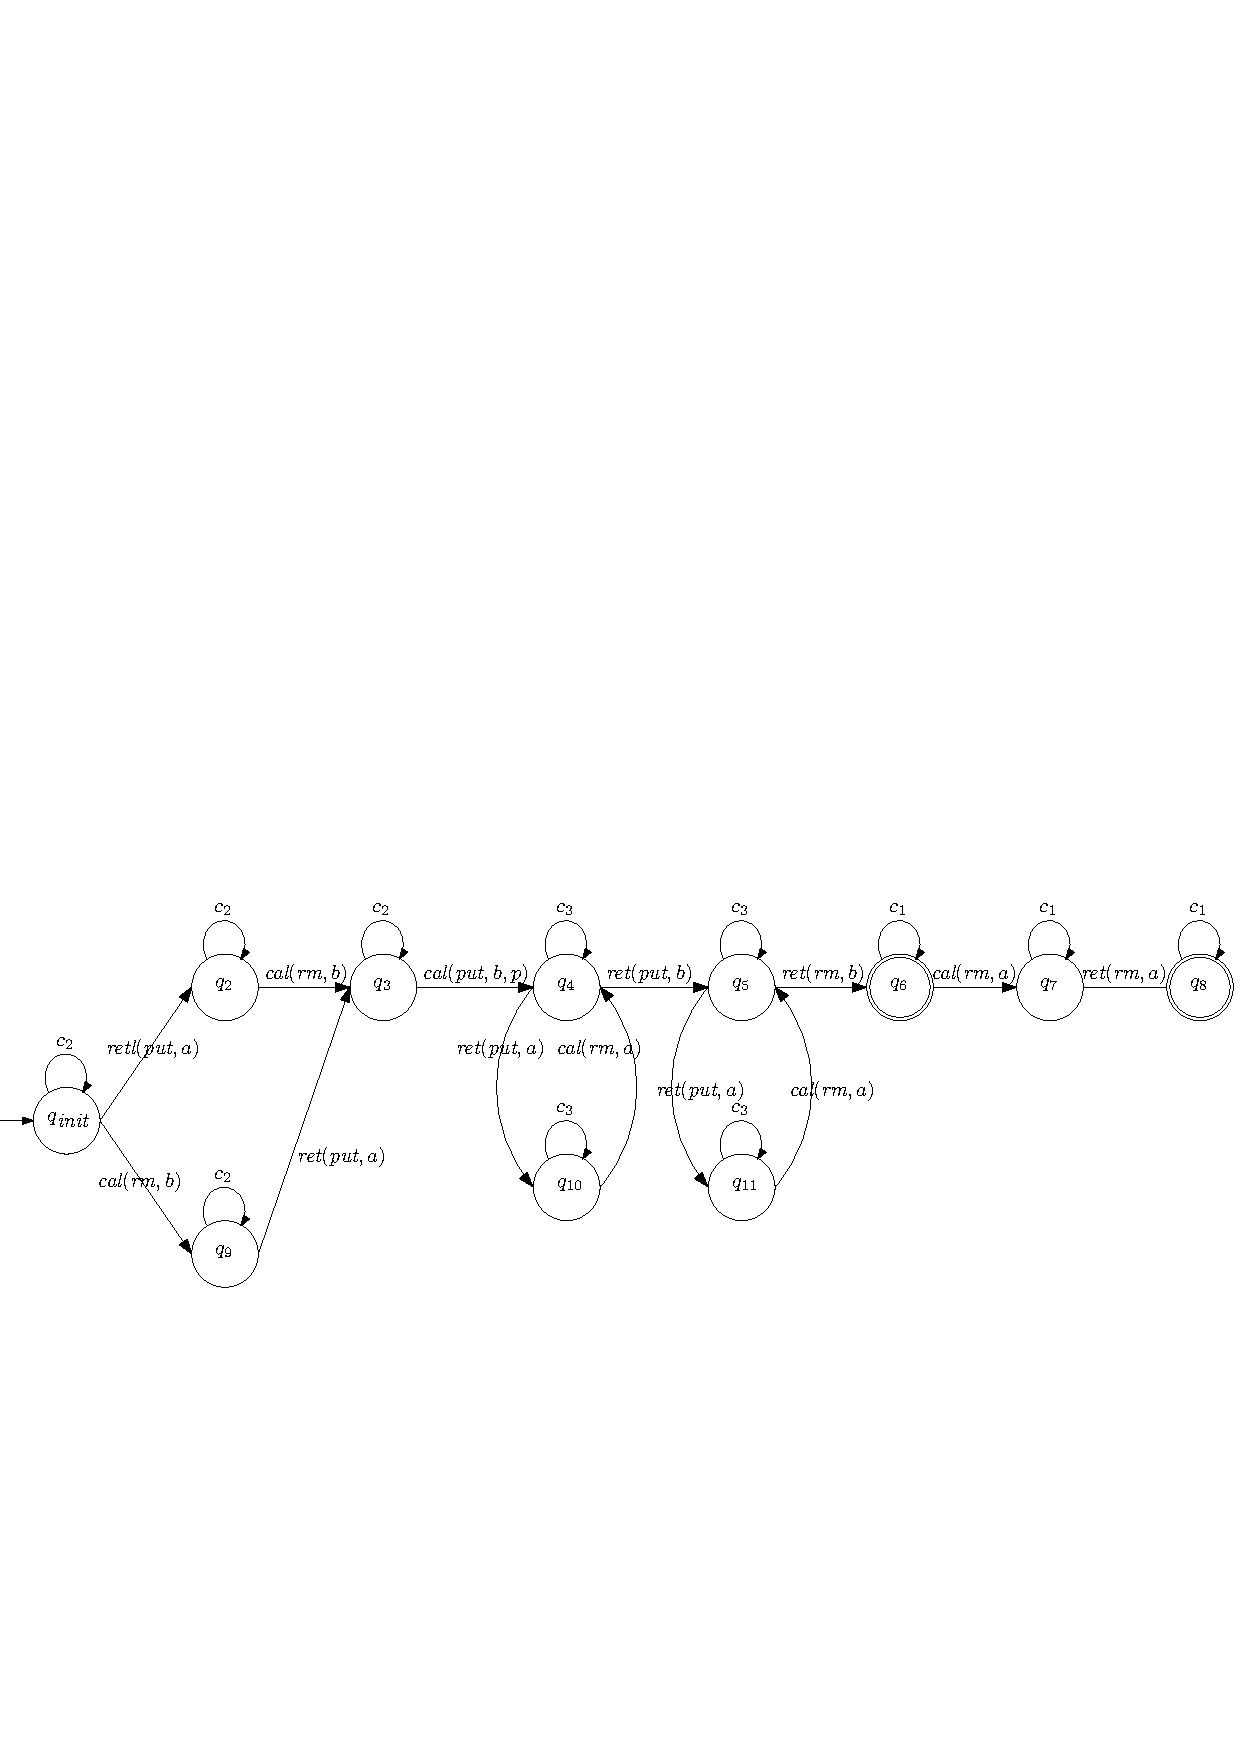
\includegraphics[width=1 \textwidth]{PIC_AUTO_UNMATCHED_Rpr1-rppr.pdf}
%\vspace{-10pt}
  \caption{Automaton $\mathcal{A}_{\textit{Rpr1-rppr}}$}
  \label{fig:automata for Rpro-rppr}
\end{figure}


The forth automaton is $\mathcal{A}_{\textit{Rpr1-rprp}}$, which is given in \figurename~\ref{fig:automata for Rpro-rprp}. In $\mathcal{A}_{\textit{Rpr1-rprp}}$, $c_2, c_3$ is same as that in $\mathcal{A}_{\textit{Rpr1-pprr}}$, and $c_4=c_1 + \textit{ret}(put,b)$. Here $\textit{rprp}$ represents that, $h' \vert_{2} = \textit{cal}(\textit{rm}) \cdot \textit{cal}(\textit{put},b,p) \cdot \textit{ret}(\textit{rm},b) \cdot \textit{ret}(\textit{put})$.

\begin{figure}[htbp]
  \centering
  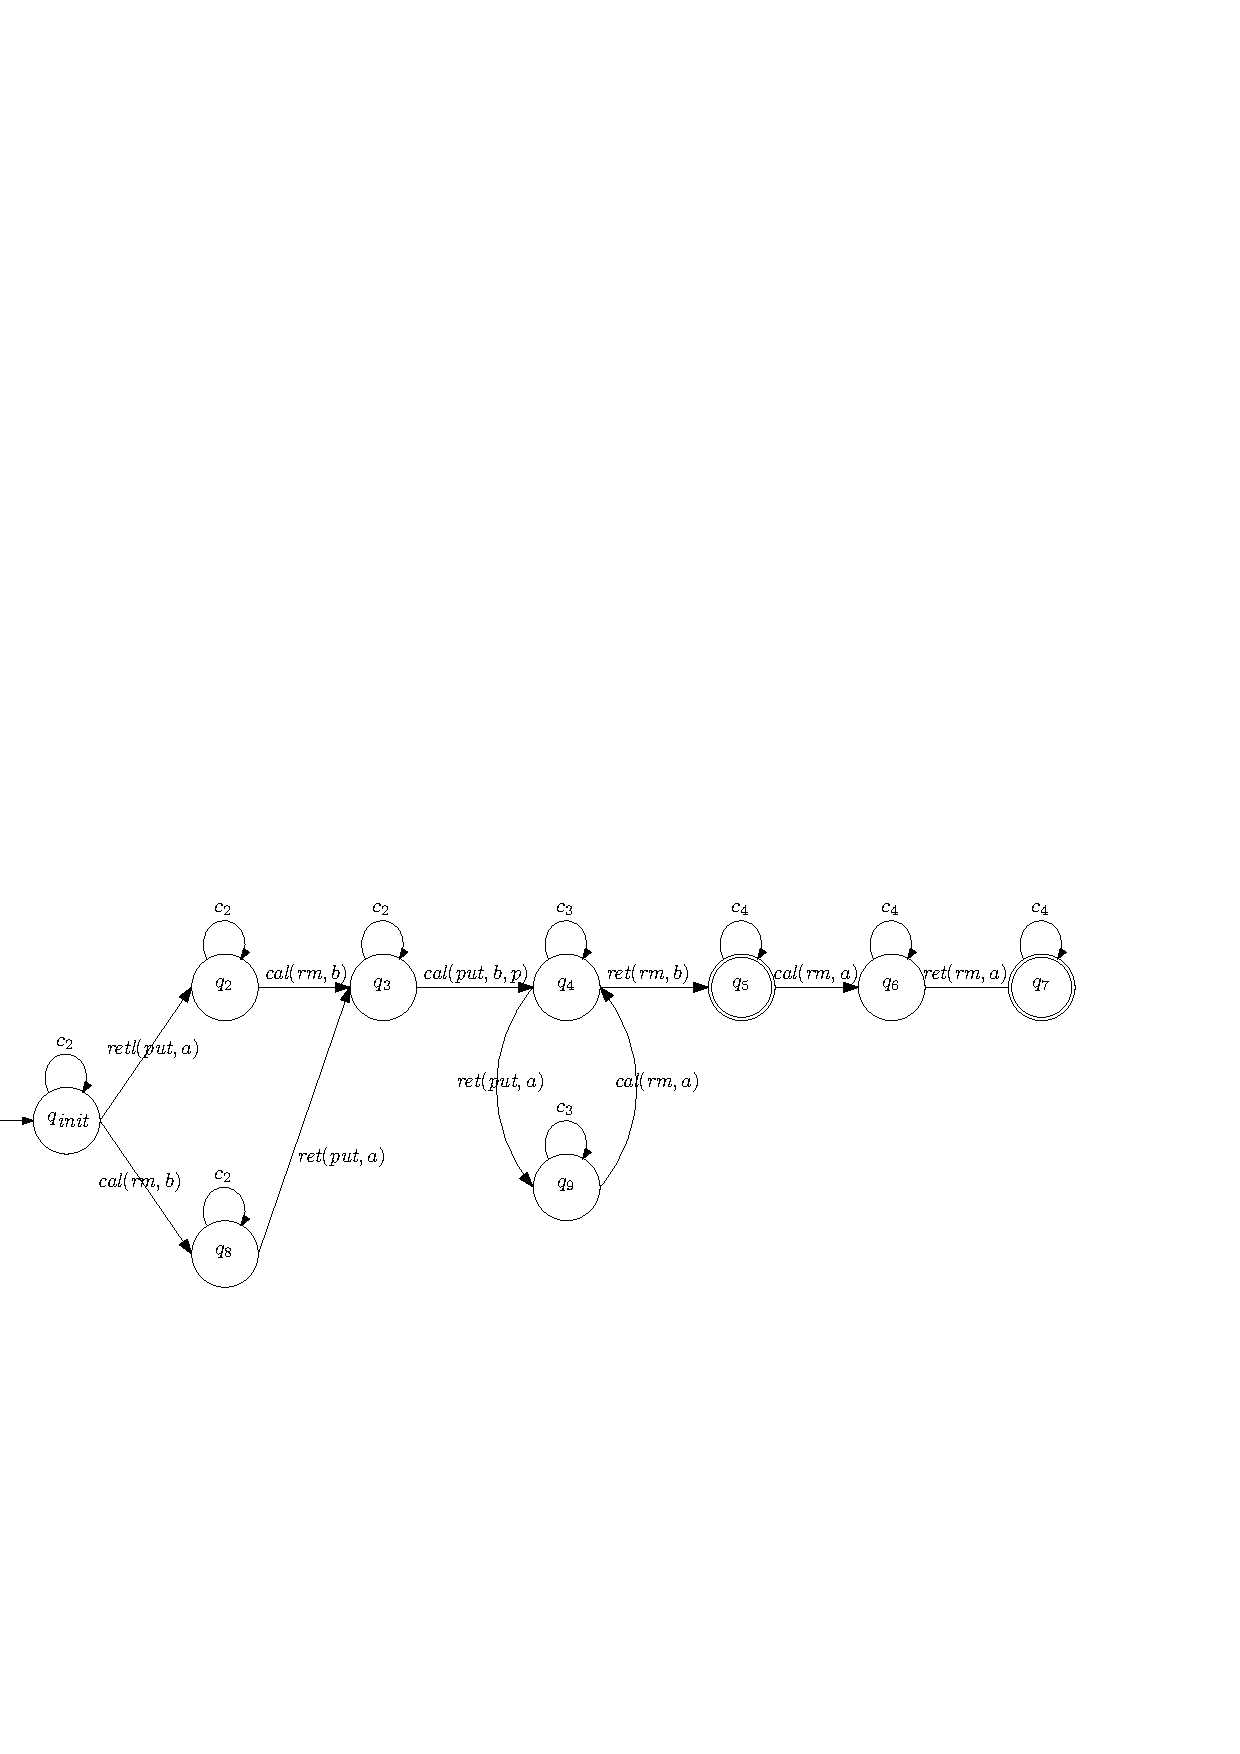
\includegraphics[width=1 \textwidth]{PIC_AUTO_UNMATCHED_Rpr1-rprp.pdf}
%\vspace{-10pt}
  \caption{Automaton $\mathcal{A}_{\textit{Rpr1-rprp}}$}
  \label{fig:automata for Rpro-rprp}
\end{figure}



Given a data-differentiated history $h$, we say that a item $x$ with priority $\textit{pri}_x$ in $h$ is covered by items $d_1,\ldots,d_m$ in $h$, if the priorities of $d_1,\ldots,d_m$ is not $\textit{pri}_x$, and

\begin{itemize}
\setlength{\itemsep}{0.5pt}
\item[-] $\textit{put}(d_m,\_)$ happens before $\textit{put}(x,\textit{pri}_x)$ or $\textit{rm}(x)$,

\item[-] For each $i < 1 \leq m$,$\textit{put}(d_{\textit{i-1}},\_)$ happens before $\textit{rm}(d_i)$,

\item[-] $\textit{rm}(x)$ happens before $\textit{rm}(d_1)$, or $\textit{rm}(d_1)$ does not exists in $h$
\end{itemize}

According to the definition of left-right constraint, in a data-differentiated history $h$, there is a cycle going through $x$, if and only if there exists items $d_1,\ldots,d_m$, such that $x$ is covered by $d_1,\ldots,d_m$.



\begin{restatable}{lemma}{Rpr1IsCoRegular}
\label{lemma:Rpr1 is co-regular}
$R_{\textit{pr1}}$ is co-regular.
\end{restatable}

\begin {proof}

Let $\textit{AutS-R}_{\textit{pr1}} = \{ \mathcal{A}_{\textit{Rpr1-1}} , \mathcal{A}_{\textit{Rpr1-pprr}}, \mathcal{A}_{\textit{Rpr1-prpr}}, \mathcal{A}_{\textit{Rpr1-rppr}}, \mathcal{A}_{\textit{Rpr1-rprp}} \}$. We need to prove that:

\noindent {\bf $\textit{fact}_1$}: Given a data-independent implementation $\mathcal{I}$, $\textit{AutS-R}_{\textit{pr1}} \cap \mathcal{I} \neq \emptyset$, if and only if there exists data-differentiated history $h \in \mathcal{I}$, $h'$ is a projection of $h$, $\textit{last}(h') = R_{\textit{pr1}}$ and $h$ does not linearizable to $\textit{MR}_{\textit{pr1}}$.

By Lemma \ref{lemma:Gap Equals Lin for Rpr1} and Lemma \ref{lemma:Gap Equals Constraint for Rpr1}, $\textit{fact}_1$ is equivalent to $\textit{fact}_2$:

\noindent {\bf $\textit{fact}_2$}: Given a data-independent implementation $\mathcal{I}$, $\textit{AutS-R}_{\textit{pr1}} \cap \mathcal{I} \neq \emptyset$, if and only if there exists data-differentiated history $h \in \mathcal{I}$, $h''$ is a projection of $h$, such that $\textit{last}(h'') = R_{\textit{pr1}}$, $\textit{put}(x,\textit{pri}_x)$ and $\textit{rm}(x)$ is in $h''$, $\textit{pri}_x$ is the maximal priority of $h''$, and one the the following case holds:

\begin{itemize}
\setlength{\itemsep}{0.5pt}
\item[-] case $1$: $\textit{rm}(x)$ happens before $\textit{put}(x,\textit{pri}_x)$,
\item[-] case $2$: $x$ is covered by some items $d_1,\ldots,d_m$ in $h''$.
\end{itemize}

\noindent The $\textit{only if}$ direction: Assume that $h_1 \in \mathcal{I}$ is accepted by $\textit{AutS-R}_{\textit{pr1}}$. By data-independence, there exists data-differentiated sequence $h_2 \in \mathcal{I}$ and a renaming function $r$, such that $h_1=r(h_2)$.

\begin{itemize}
\setlength{\itemsep}{0.5pt}
\item[-] If $h_1$ is accepted by $\mathcal{A}_{\textit{Rpr1-1}}$: Let $d_1$ a item in $h_2$ such that $r(d_1)=b$ and let $h'' = h_2 \vert_{ \{ d_1 \} }$. $d_1$ is the item with maximal priority in $h''$. It is obvious that $\textit{last}(h'') = R_{\textit{pr1}}$ and $\textit{rm}(d_1)$ happens before $\textit{put}(d_1,\_)$ in $h''$.

\item[-] If $h_1$ is accepted by $\mathcal{A}_{\textit{Rpr1-pprr}}$, $\mathcal{A}_{\textit{Rpr1-prpr}}$, $\mathcal{A}_{\textit{Rpr1-rppr}}$, or $\mathcal{A}_{\textit{Rpr1-rprp}}$: Let $d_0$ be a item in $h_2$ such that $r(d_0)=b$, let $d_1,\ldots,d_m$ be the items in $h_2$ such that $r(d_i)=a$ for each $1 \leq i \leq m$. Let $h'' = h_1 \vert_{ \{ d_0, d_1, \ldots, d_m \} }$. It is obvious that the priority of $d_0$ is larger than the priorities of other operations in $h''$, and then $\textit{last}(h'') = R_{\textit{pr1}}$. It is easy to see that $d_0$ is covered by $d_1,\ldots,d_m$.
\end{itemize}

\noindent The $\textit{if}$ direction: Assume that there exists such $h$, $h''$, $x$ and $\textit{pri}_x$. Since $\textit{last}(h'') = R_{\textit{pr1}}$, $\textit{pri}_x$ is larger than the priorities of other operations in $h''$. Then,

\begin{itemize}
\setlength{\itemsep}{0.5pt}
\item[-] If case $1$ holds: Then, $\textit{rm}(x)$ happens before $\textit{put}(x,\textit{pri}_x)$ in $h''$. Let $h_1$ be obtained from $h$ by renaming $x$ to $b$ and renaming all other items to $a$. By data-independence, $h_1 \in \mathcal{I}$, and it is easy to see that $h_1$ is accepted by $\mathcal{A}_{\textit{Rpr1-1}}$.
\item[-] case $2$: Then, $x$ is covered by some items $d_1,\ldots,d_m$ in $h''$. There are four possibilities of $h'' \vert_{ \{ x \} }$: (1) $\textit{call}(\textit{put},x,\textit{pri}_x) \cdot \textit{ret}(\textit{put}) \cdot \textit{call}(\textit{rm}) \cdot \textit{ret}(\textit{rm},x)$, (2) $\textit{call}(\textit{put},x,\textit{pri}_x) \cdot \textit{call}(\textit{rm}) \cdot \textit{ret}(\textit{put}) \cdot \textit{ret}(\textit{rm},x)$, (3) $\textit{call}(\textit{rm}) \cdot \textit{call}(\textit{put},x,\textit{pri}_x) \cdot \textit{ret}(\textit{put}) \cdot \textit{ret}(\textit{rm},x)$ and (4) $\textit{call}(\textit{rm}) \cdot \textit{call}(\textit{put},x,\textit{pri}_x) \cdot \textit{ret}(\textit{rm},x) \cdot \textit{ret}(\textit{put})$.

    Let $h_1$ be obtained from $h$ by renaming $x$ into $b$, renaming $d_1,\ldots,d_m$ into $a$ and renaming other items into $c$. We can prove that $h_1$ is accepted by $\mathcal{A}_{\textit{Rpr1-pprr}}$, $\mathcal{A}_{\textit{Rpr1-prpr}}$, $\mathcal{A}_{\textit{Rpr1-rppr}}$ or $\mathcal{A}_{\textit{Rpr1-rprp}}$.

    For example, if $h'' \vert_{ \{ x \} } = \textit{call}(\textit{put},x,\textit{pri}_x) \cdot \textit{ret}(\textit{put}) \cdot \textit{call}(\textit{rm}) \cdot \textit{ret}(\textit{rm},x)$, and $\textit{ret}(\textit{rm},d_m)$ is before $\textit{call}(\textit{put},x,\textit{pri}_x)$ and is after $\textit{ret}(\textit{put},x)$ in $h''$. Then in  $\mathcal{A}_{\textit{Rpr1-pprr}}$, $h_1$ is accepted by transitions from $q_{\textit{init}}$ to $q_2$ to $q_{11}$ and finally to $q_7$ (if $\textit{rm}(d_1)$ does not exists in $h''$) or $q_9$ (if $\textit{rm}(d_1)$ exists in $h''$).
\end{itemize}

This completes the proof of this lemma. \qed
\end {proof}




\subsection{Co-Regular of $R_{\textit{pr2}}$}
\label{subsec:co-regular of Rpr2}

An automaton $\mathcal{A}_{\textit{FIFO-Sig-Pri}}$ is given in \figurename~\ref{fig:automata for FIFO of single priority}. In \figurename~\ref{fig:automata for FIFO of single priority}, let $c_1= \textit{cal}(\textit{put},c,\textit{anyPri}),\textit{ret}(\textit{put},c)$, $\textit{cal}(\textit{rm},c),\textit{ret}(\textit{rm},c)$, $c_2 = c_1 + \textit{ret}(\textit{put},b)$, and $c_3 = c_2 + \textit{cal}(\textit{rm},a) + \textit{ret}(\textit{rm},a)$.

\begin{figure}[htbp]
  \centering
  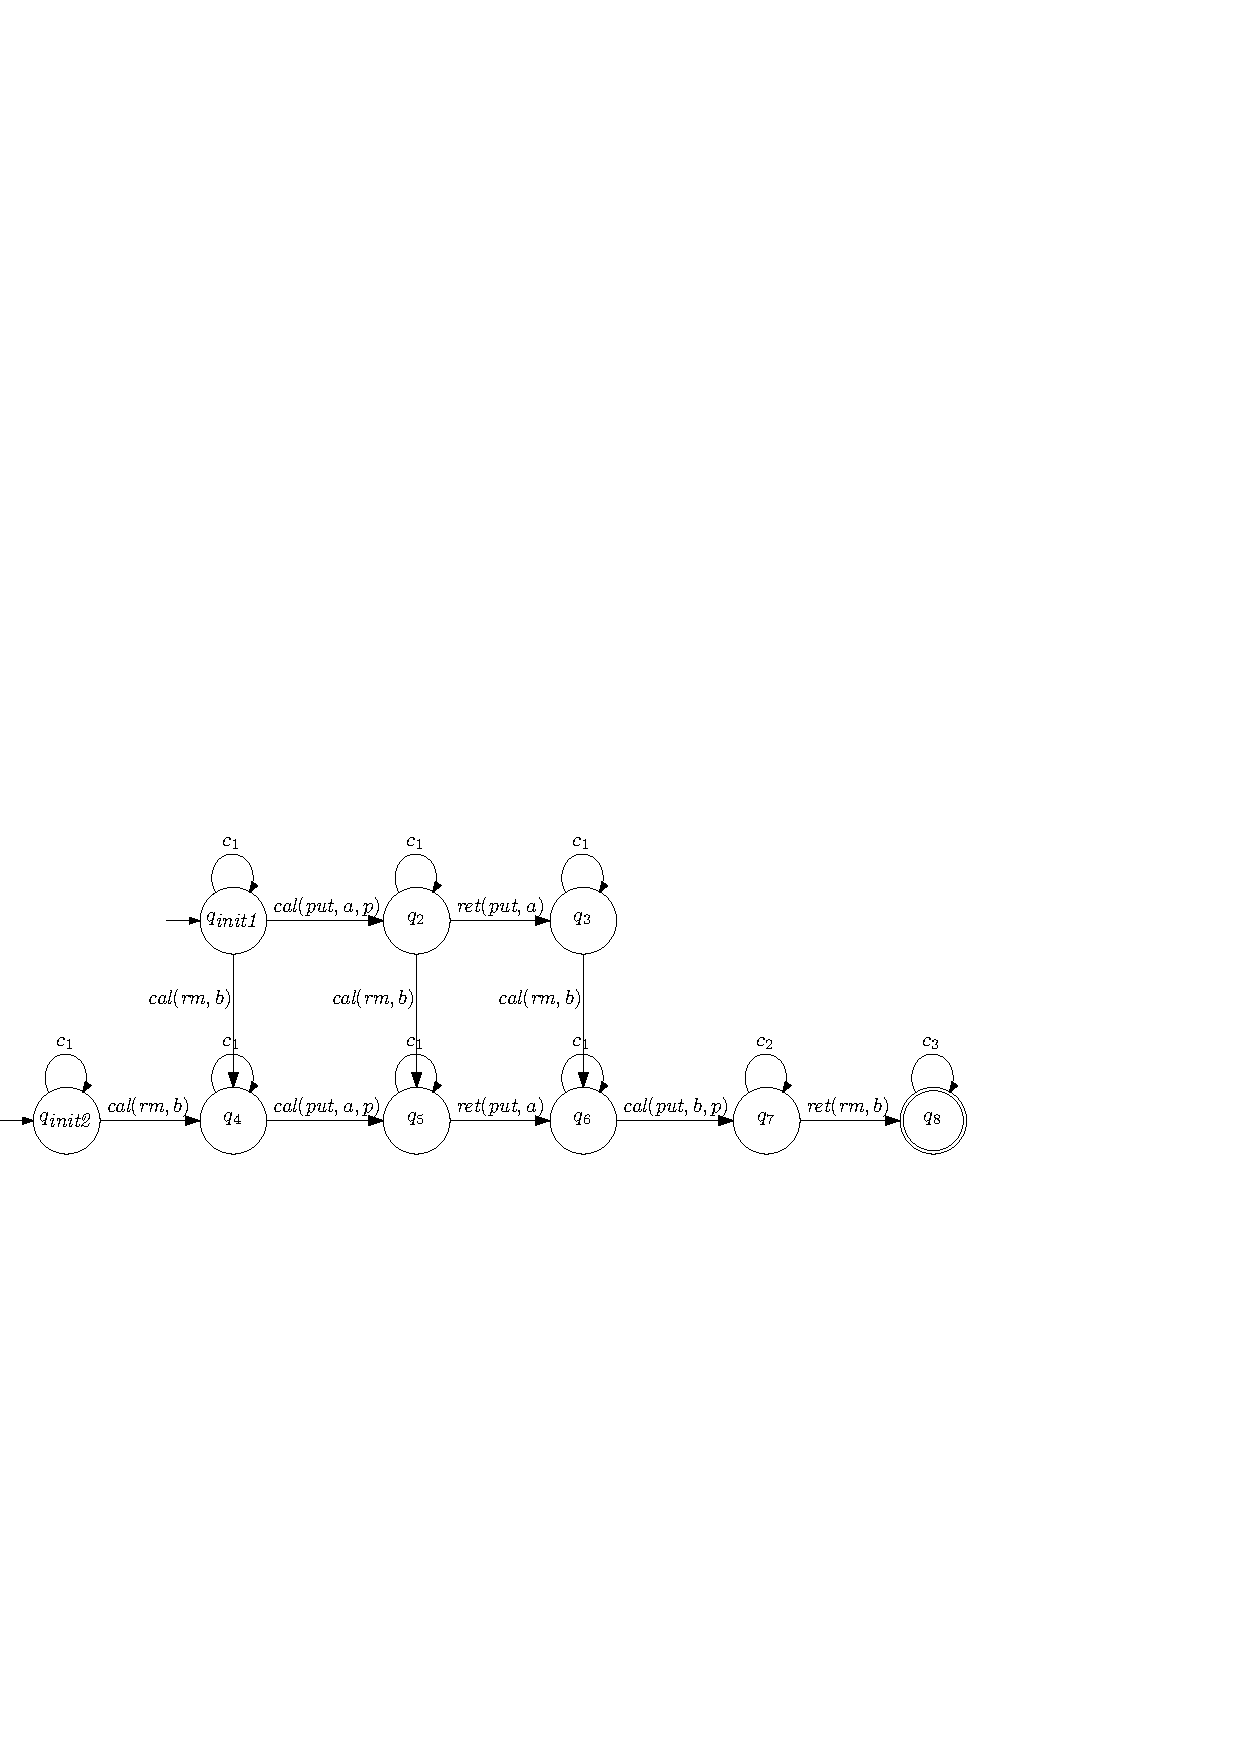
\includegraphics[width=0.8 \textwidth]{PIC_AUTO_QUEUE_FOR_SINGLE_PRI.pdf}
%\vspace{-10pt}
  \caption{Automaton $\mathcal{A}_{\textit{FIFO-Sig-Pri}}$}
  \label{fig:automata for FIFO of single priority}
\end{figure}

According to \cite{Bouajjani:2015}, given a data-independent set $S$ of queue executions, whether every sequence $s$ in $S$ is linearizable to queue can be reduced into checking emptiness of intersection of $S$ and several finite automata. Let $\textit{transToQueue}(h)$ be a sequence $h'$ that is generated from $h$ by transforming $\textit{put}$ and $\textit{rm}$ into $\textit{enq}$ and $\textit{deq}$, respectively, and then discarding priorities. A priority queue history is called single-priority, if all of its items has only one priority. The following lemma states that we can also use finite automata to check ``first in first out property'' for single-priority sub-sequence of priority queue history.

\begin{restatable}{lemma}{AutoForPQwithSignlePri}
\label{lemma:automata for priority queue with single priority}

Given a data-independent implementations $\mathcal{I}$ of priority queue, let $\mathcal{A} = \{ \mathcal{A}_{\textit{unmRm1}}, \mathcal{A}_{\textit{Rpr0-1}}, \mathcal{A}_{\textit{unmRm2}}, \mathcal{A}_{\textit{FIFO-Sig-Pri}} \}$, then,

$\mathcal{I} \cap \mathcal{A} \neq \emptyset$, if and only if there exists $e \in \mathcal{I}$, $e' \in \textit{proj}(e)$, such that $e'$ is single-priority, and $\textit{transToQueue}(e')$ does not linearizable to queue.
\end{restatable}

\begin {proof}

According to \cite{Bouajjani:2015}, checking linearizable with respect to queue can be reduced into checking the following three conditions for data-differentiated histories:

\begin{itemize}
\setlength{\itemsep}{0.5pt}
\item[-] $\textit{deq}(a)$ happens before $\textit{enq}(a)$ (or $\textit{enq}(a)$ does not exist) for some item $a$,

\item[-] there are two or more $\textit{deq}(a)$ for some item $a$,

\item[-] $\textit{enq}(a)$ happens before $\textit{enq}(b)$, and $\textit{deq}(b)$ happens before $\textit{deq}(a)$ (or $\textit{deq}(a)$ does not exists) for some items $a,b$.
\end{itemize}

It is not hard to see that (1) the first condition is dealt with by $\mathcal{A}_{\textit{unmRm1}}$ (if $\textit{put}(a,\_)$ does not exist) and $\mathcal{A}_{\textit{Rpr0-1}}$ (if $\textit{put}(a,\_)$ exists), (2) the second condition is dealt with by $\mathcal{A}_{\textit{unmRm2}}$, and (3) the third condition is dealt with by $\mathcal{A}_{\textit{FIFO-Sig-Pri}}$. \qed
\end {proof}

By Lemma \ref{lemma:automata for priority queue with single priority}, from now on, it is safe for us to assume that, for each data-differentiated priority queue history $h$ and each $h'$ of projection of $h$, if $h'$ is single-priority, then $\textit{transToQueue}(h')$ is linearizable to queue. One consequence of this assumption is that, in $h'$, there does not exists an item $a$, such that $\textit{rm}(a)$ happens before $\textit{put}(a)$.

By the proof of Lemma \ref{lemma:Rpr1 is co-regular}, with the help of $\mathcal{A}_{\textit{Rpr1-pprr}}, \mathcal{A}_{\textit{Rpr1-prpr}}, \mathcal{A}_{\textit{Rpr1-rppr}}$ and $\mathcal{A}_{\textit{Rpr1-rprp}}$, from now on, we can safely assume that given a data-differentiated history $h$ and operations $\textit{put}(x,\textit{pri}_x)$ and $\textit{rm}(x)$ in $h$, there does not exists any items $d_1,\ldots,d_m$, such that $x$ is not covered by items $d_1,\ldots,d_m$ and the priority of $d_1,\ldots,d_m$ is less that $x$.


However, above two assumptions are not enough for imply the linearizability to priority queue. One example is shown in \figurename~\ref{fig:history introduct ob order1}. The history $h$ of \figurename~\ref{fig:history introduct ob order1} is not linearizable, even if $h \vert_{1}$ and $h \vert_{2}$ are both linearizable, and either $a$ or $b$ is covered by other items. One explanation is that, since $\textit{put}(b,1)$ happens before $\textit{put}(a,1)$, in choosing linearization points, we should make $\textit{rm}(b)$ before $\textit{rm}(a)$. However, to satisfy the requirements of $R_{\textit{pr2}}$, the linearization points of $\textit{rm}(a)$ can only locates in the interval from $\textit{ret}(\textit{rm},d)$ to $\textit{cal}(\textit{put},e,2)$. But, $\textit{rm}(b)$ is after this entire interval, and we can not locate the linearization point of $\textit{rm}(b)$ in this interval. When there is no such phenomenon, such as the history in \figurename~\ref{fig:history introduct ob order2}, the history becomes linearizable.

\begin{figure}[htbp]
  \centering
  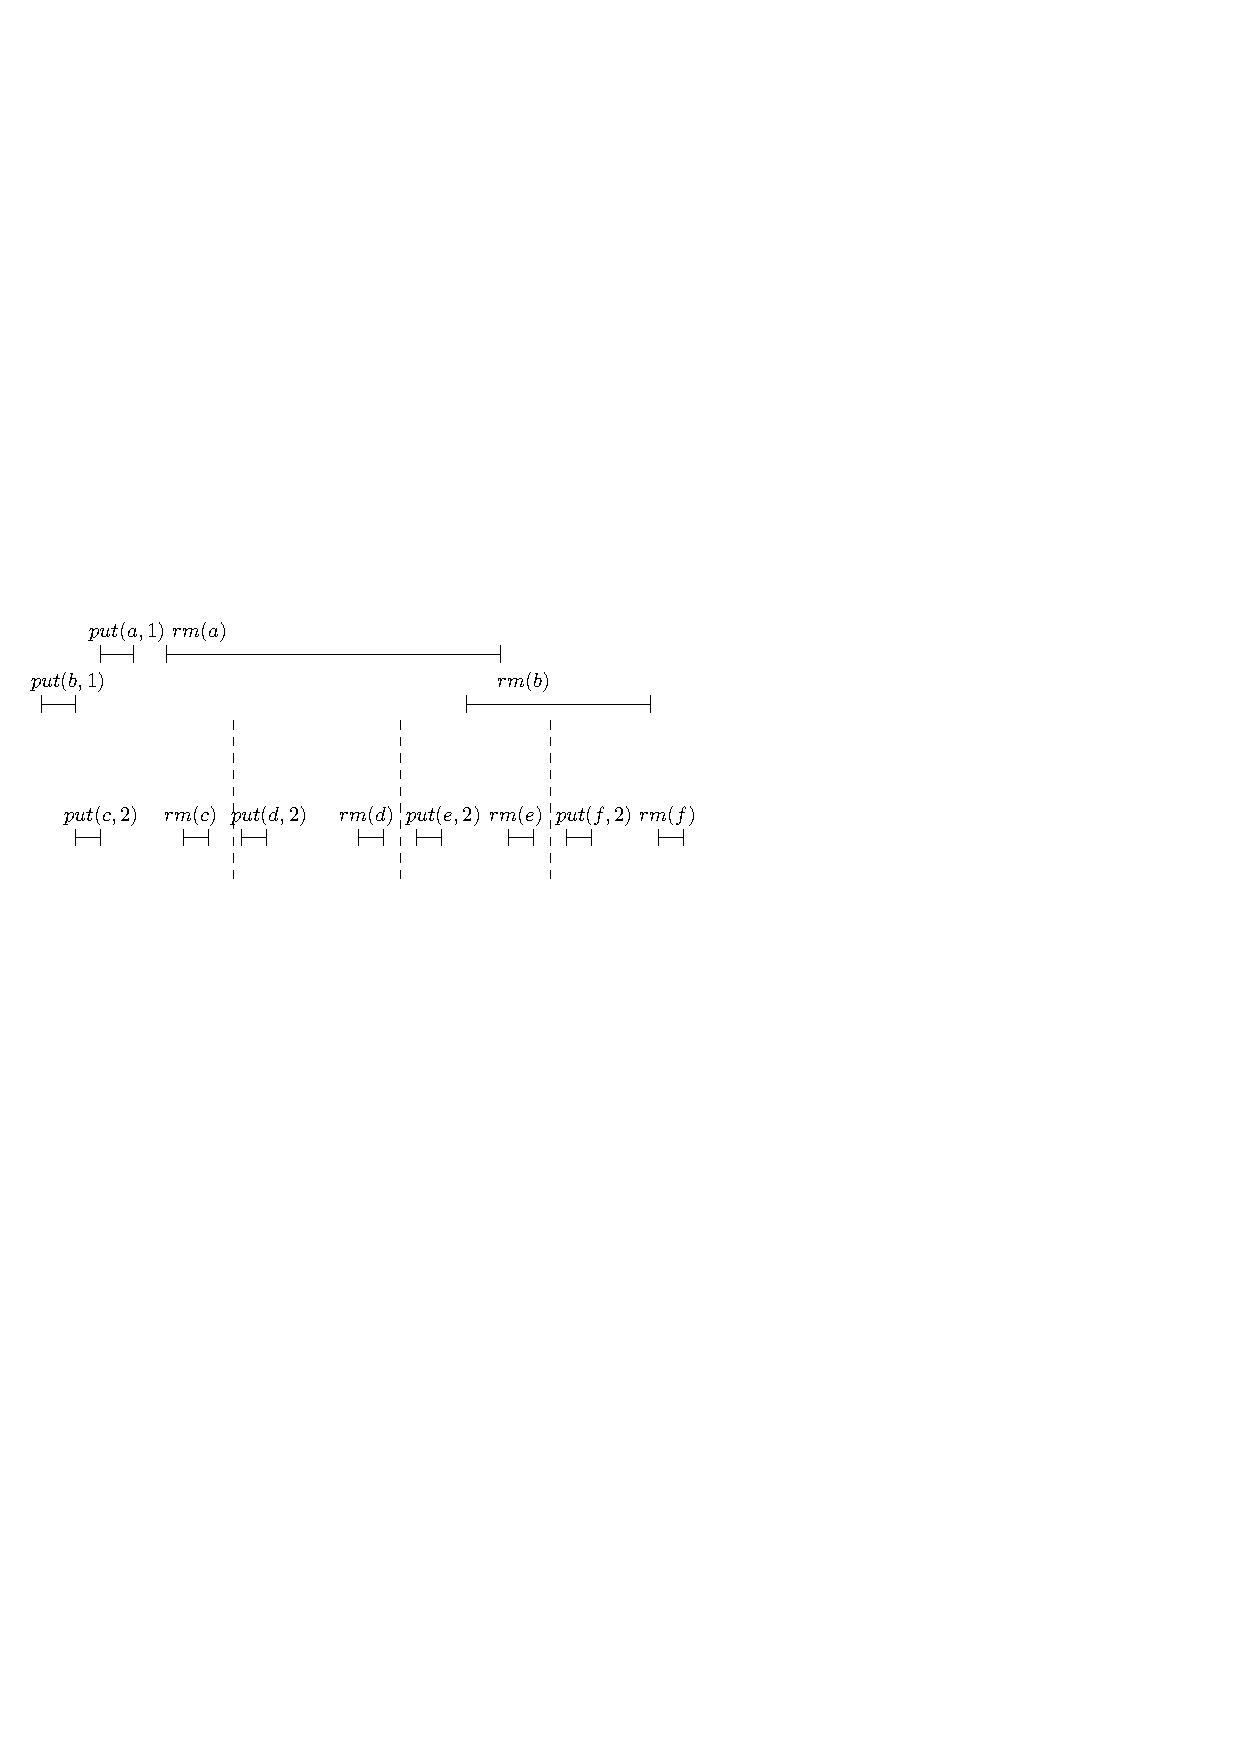
\includegraphics[width=0.6 \textwidth]{PIC-HIS-INTRO-OB-ORDER1.pdf}
%\vspace{-10pt}
  \caption{above assumptions do not implies linearizability (1)}
  \label{fig:history introduct ob order1}
\end{figure}


%\begin{figure}[htbp]
%  \centering
%  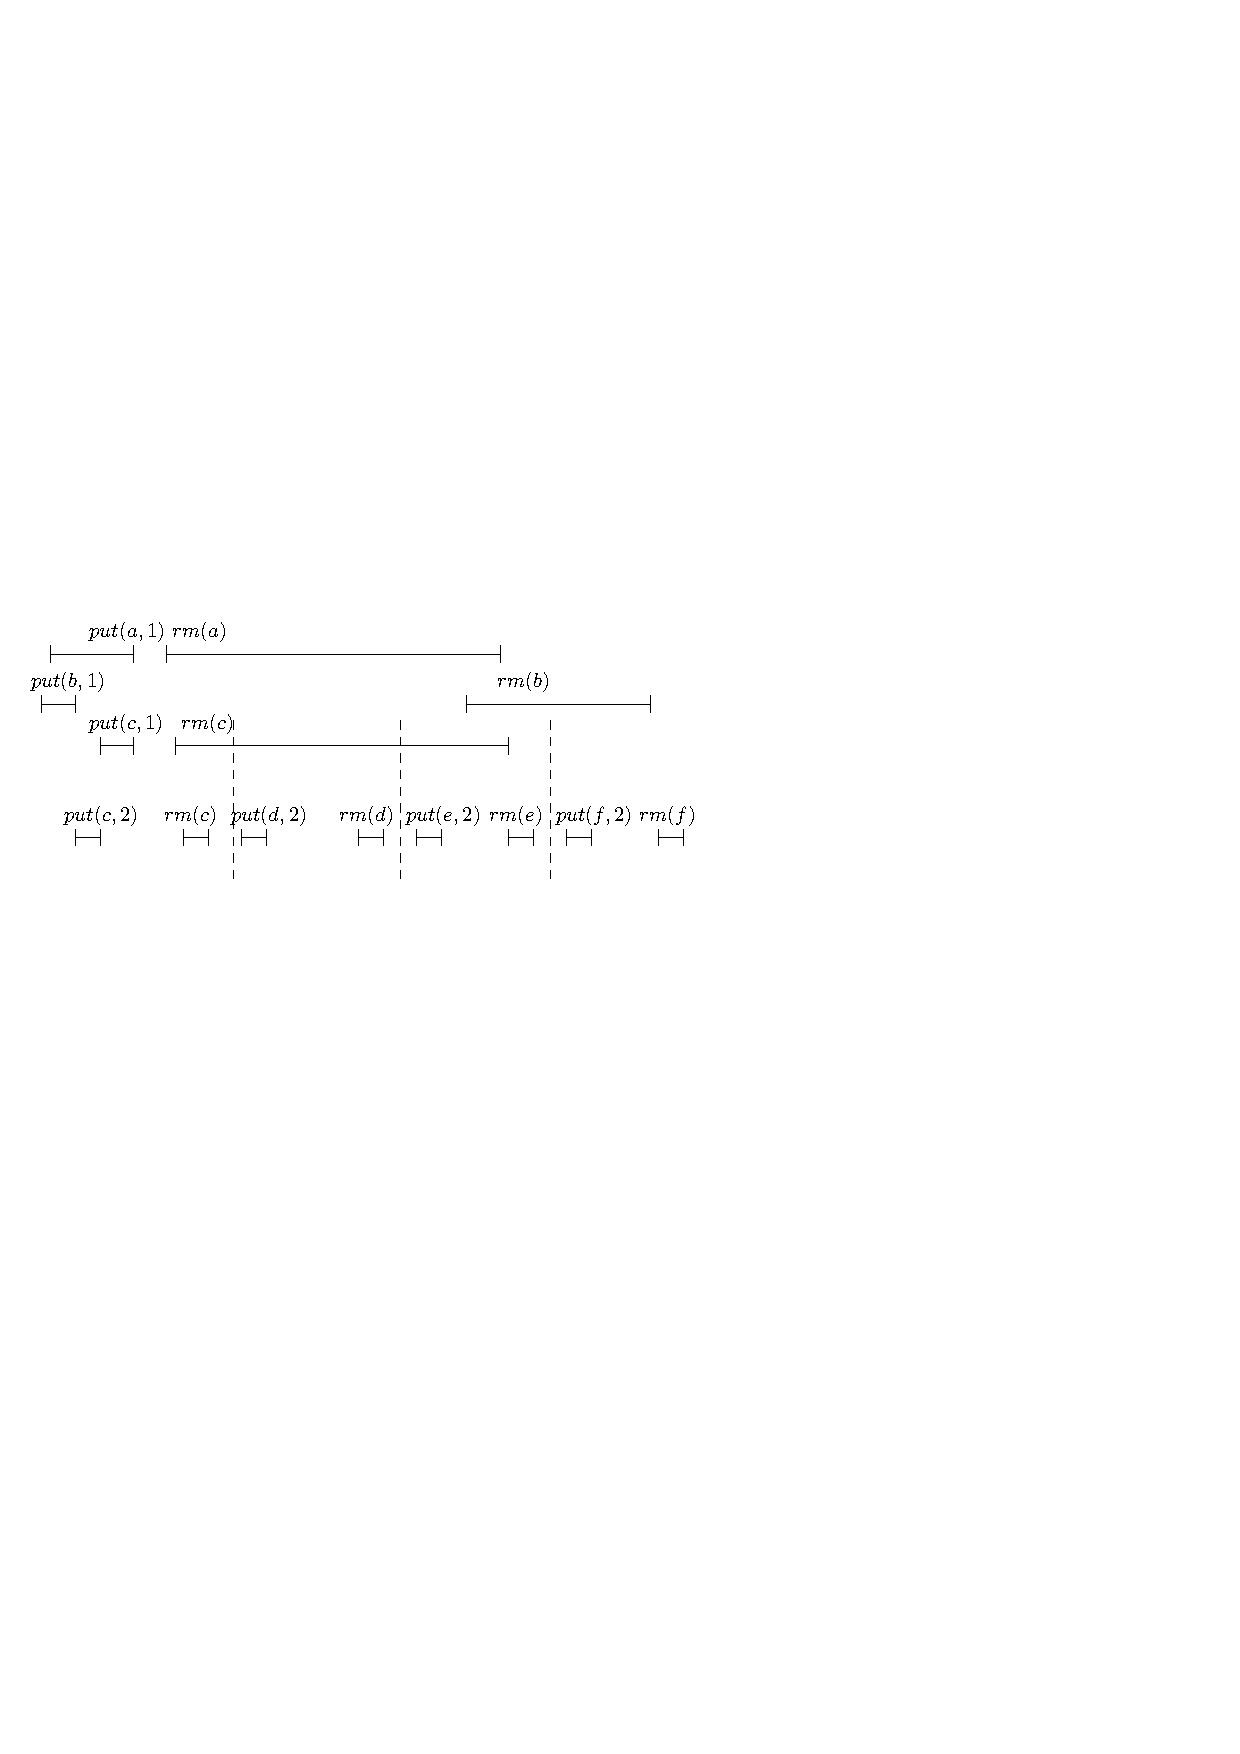
\includegraphics[width=0.6 \textwidth]{PIC-HIS-INTRO-OB-ORDER3.pdf}
%\vspace{-10pt}
%  \caption{above assumptions do not implies linearizability (2)}
%  \label{fig:history introduct ob order1}
%\end{figure}


\begin{figure}[htbp]
  \centering
  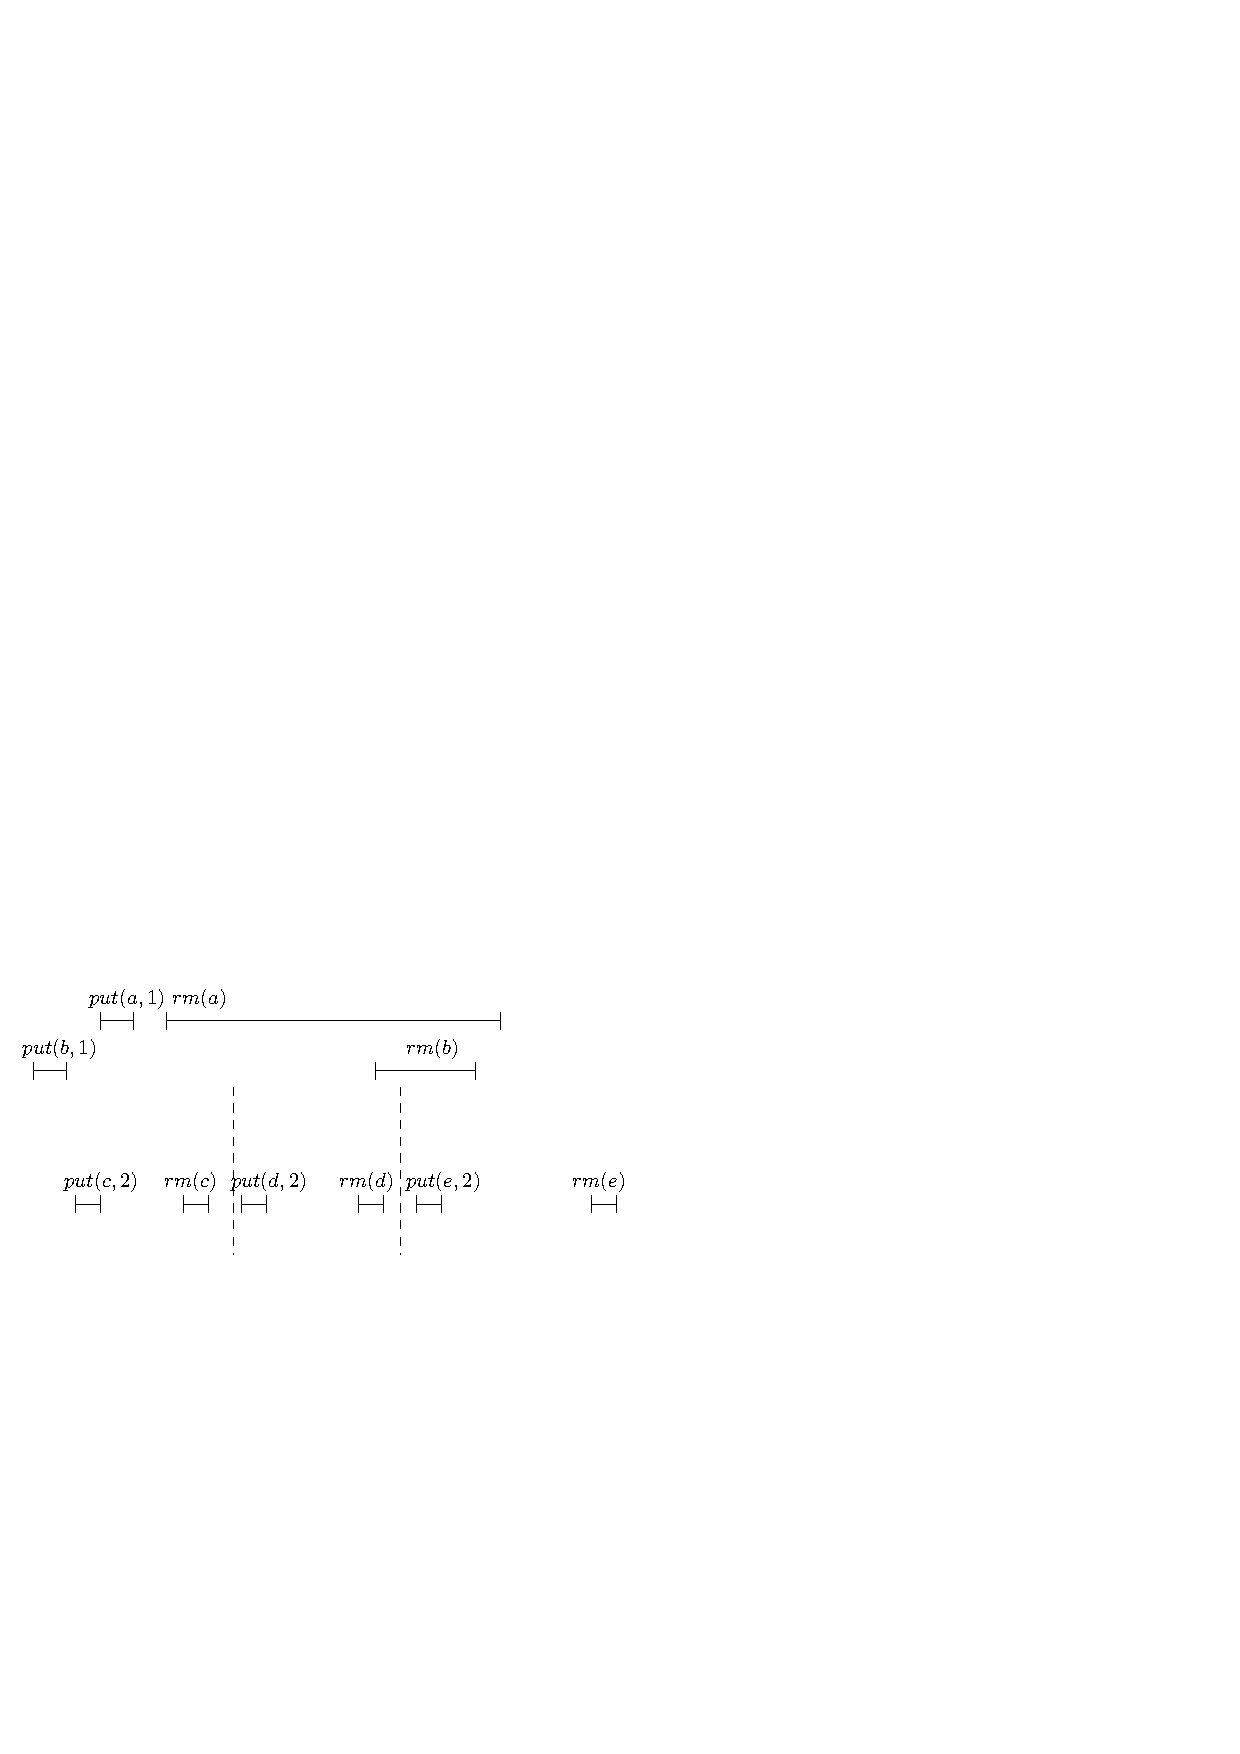
\includegraphics[width=0.6 \textwidth]{PIC-HIS-INTRO-OB-ORDER2.pdf}
%\vspace{-10pt}
  \caption{above assumptions do not implies linearizability (2)}
  \label{fig:history introduct ob order2}
\end{figure}

In the following part of this subsection, we use $<_{\textit{ob}}$ order for the case when we can infer that an item is inserted earlier than another item, and we use gap-point to represent the intervals when it is possible to locate linearizaton points of $\textit{rm}(a)$.

\begin{definition}[gap-point for matched $\textit{put}$ and $\textit{rm}$ operations]\label{def:gap-point for matched put and rm operations}

Given a data-differentiated history $h$ and two operations $\textit{put}(x,\textit{pri}_x),\textit{rm}(x)$ of $h$, we say $o$ is a gap-point of $\textit{put}(x,\textit{pri}_x)$ and $\textit{rm}(x)$, if we can obtain a sequence $\textit{gapPSeq}(h)$ from $h$ by adding $o$ to some locations between actions of $h$, and satisfies that,

\begin{itemize}
\setlength{\itemsep}{0.5pt}
\item[-] In $\textit{gapPSeq}(h)$, $o$ is after $\textit{call}(\textit{put},x,\textit{pri}_x)$ and $\textit{call}(\textit{rm},x)$, and is before $\textit{ret}(\textit{rm},x)$.
\item[-] For each item $y$ with non-$\textit{pri}_x$ priority in $\textit{gapPSeq}(h)$. If $\textit{put}(y,\_)$ and $\textit{rm}(y)$ is in $h$, then it can not be the case that $\textit{ret}(\textit{put},y,\_)$ is before $o$ and $\textit{call}(\textit{rm},x)$ is after $o$; Else if $\textit{put}(y,\_)$ is in $h$ and $\textit{rm}(y)$ is not in $h$, then it can not be the case that $\textit{ret}(\textit{put},y,\_)$ is before $o$;
\end{itemize}

We say that $o$ is a gap-point of priority $\textit{pri}_x$, if we can obtain a sequence $\textit{gapPSeq}(h)$ from $h$ by adding $o$ to some locations between actions of $h$, and satisfies only the latter requirement.
\end{definition}




\begin{restatable}{lemma}{GapEqualsGapPoint}
\label{lemma:gap eqals the existence of gap point}
Given a data-differentiated history $h$ and two operations $\textit{put}(x,\textit{pri}_x)$ and $\textit{rm}(x)$ of $h$. There is a gap on $\textit{put}(x,\_)$ and $\textit{rm}(x)$ in $h$, if and only if there is a gap-point $o$ of $\textit{put}(x,\_)$ and $\textit{rm}(x)$ in $h$.
\end{restatable}

\begin {proof}

To prove the $\textit{only if}$ direction, we need to prove that: if there is no gap-point of $\textit{put}(x,\_)$ and $\textit{rm}(x)$ in $h$, then there is no gap on $\textit{put}(x,\_)$ and $\textit{rm}(x)$ in $h$.

We prove this by contradiction. Assume that there is no gap-point of $\textit{put}(x,\_)$ and $\textit{rm}(x)$ in $h$, but there is a gap on $\textit{put}(x,\_)$ and $\textit{rm}(x)$ in $h$. Since there is no gap-point of $\textit{put}(x,\_)$ and $\textit{rm}(x)$ in $h$, in the time interval starts from $\textit{cal}(\textit{put},x,\textit{pri}_x)$ and $\textit{cal}(\textit{rm},x)$ and ends at $\textit{ret}(\textit{rm},x)$, there is always some item with non-$\textit{pri}_x$ priority in priority queue. Therefore, it is not hard to prove that there is a cycle going through the left-right constraint of $\textit{put}(x,\_)$ and $\textit{rm}(x)$, and by Lemma \ref{lemma:Gap Equals Constraint for Rpr0}, there is no gap of $\textit{put}(x,\_)$ and $\textit{rm}(x)$ in $h$, which contradicts that there is a gap on $\textit{put}(x,\_)$ and $\textit{rm}(x)$ in $h$.

To prove the $\textit{if}$ direction, assume that there is a gap-point $o$ of $\textit{put}(x,\_)$ and $\textit{rm}(x)$ in $h$ and let $h_1$ be the sequence in definition of gap-point, which is generated from $h$ by adding $o$ into $h$. Let sequence $h_2$ be a sequence of call, return and operations, such that the projection of $h_2$ into call and return actions is $h$. $h_2$ is generated as follows:

\begin{itemize}
\setlength{\itemsep}{0.5pt}
\item[-] First, from $h_1$, transform the point $o$ into $\textit{rm}(x)$.

\item[-] Then for all the other items $y$, (1) adding an operation $\textit{put}(y,p)$ at some position between $\textit{call}(\textit{put},y,\_)$ and $\textit{ret}(\textit{put},y)$, and (2) adding an operation $\textit{rm}(y)$ at some position between $\textit{call}(\textit{rm},y)$ and $\textit{ret}(\textit{rm},y)$.

\item[-] For all items $z$ with the same priority as $x$, the positions for adding operations of $z$ into $h$ is arbitrary (but need to satisfy above restriction. In the following we implicitly require this).

\item[-] For all items $z$ whose priority is different from that of $x$,

    \begin{itemize}
    \setlength{\itemsep}{0.5pt}

    \item[-] If $\textit{put}(z,\_) <_{\textit{hb}} \textit{rm}(z)$, and $\textit{ret}(\textit{put},z,\_)$ is before $o$ in $h_1$: Then in $h_2$, $\textit{rm}(z,\_)$ is just after $\textit{call}(\textit{rm},z)$.

    \item[-] If $\textit{put}(z,\_) <_{\textit{hb}} \textit{rm}(z)$, and $o$ is before $\textit{ret}(\textit{put},z,\_)$ $h_1$: Then in $h_2$, $\textit{put}(z,\_)$ is just before $\textit{ret}(\textit{put},z)$.

    \item[-] Otherwise, we can see that $\textit{put}(z,\_)$ and $\textit{rm}(z)$ overlaps in $h$. Then we add $o_1=\textit{put}(z,\_)$ and $o_2=\textit{rm}(z)$ in the time interval of interleaving of $\textit{put}(z,\_)$ and $\textit{rm}(z)$ overlaps in $h$, make sure $o_2$ next to $o_1$, and make sure either both of them is before $\textit{rm}(x)$ or both of them is after $\textit{rm}(x)$ in $h_2$.
    \end{itemize}
\end{itemize}

According to the definition of gap-point, it is not hard to see that we can construct such $h_2$. Let $l$ be the projection of $h_2$ into operations, and $l'$ be the projection of $l$ into $x$ and all items that has priorities not equals that of $x$. Let $l'= u \cdot \textit{put}(x,\_) \cdot v \cdot \textit{rm}(x) \cdot w$. It is easy to see that $h \sqsubseteq l$, and $u \cdot v$ contains matched $\textit{put}$ and $\textit{rm}$ operations. Let $L$, $M$ and $R$ be the set of operations in $u$, $v$ and $w$, respectively. Then it is obvious that $L$, $M$ and $R$ is a gap of $\textit{put}(x,\_)$ and $\textit{rm}(x)$ in $h$. \qed
\end {proof}

Given a data-differentiated history $h$ and two items $a,b$, we say that $a <_{\textit{ob}} b$, if the priority of $a$ and $b$ is the same, and one of the following cases holds:

\begin{itemize}
\setlength{\itemsep}{0.5pt}
\item[-] Type $A$: $\textit{put}(a,\_)$ happens before $\textit{put}(b,\_)$ in $h$,

\item[-] Type $B$: $\textit{rm}(a)$ happens before $\textit{rm}(b)$ in $h$,

\item[-] Type $C$: $\textit{rm}(a)$ happens before $\textit{put}(b,\_)$ in $h$,
\end{itemize}

Let $<_{\textit{ob}}^*$ be the transitive closure of $<_{\textit{ob}}$. Intuitively, $a <_{\textit{ob}} b$ means that $a$ should be inserted earlier than $b$, and $a <_{\textit{ob}}^* b$ means that we can infer that $a$ should be inserted earlier than $b$ with the help of other items. We can explicitly write $a <_{\textit{ob}}^A b$ to mean that $a <_{\textit{ob}} b$ and the reason is that $\textit{put}(a,\_)$ happens before $\textit{put}(b,\_)$. Similarly, we can explicitly write $a <_{\textit{ob}}^B b$ and $a <_{\textit{ob}}^C b$ to mean that $a <_{\textit{ob}} b$ and the reason is that $\textit{put}(a,\_)$ happens before $\textit{put}(b,\_)$ and $\textit{rm}(a)$ happens before $\textit{put}(b,\_)$, respectively.

According to the definition of $<_{\textit{ob}}^*$, if $a <_{\textit{ob}}^* b$, then there exists $c_1,\ldots,c_n$, such that $a <_{\textit{ob}} c_1 <_{\textit{ob}} \ldots <_{\textit{ob}} b$. The following lemma states that, the number of intermediate items $c_i$ is in fact bounded.


\begin{restatable}{lemma}{OBOrderHasBoundedLength}
\label{lemma:ob order has bounded length}
Given a data-differentiated history $h$. Assume that $a <_{\textit{ob}} a_1 <_{\textit{ob}} \ldots <_{\textit{ob}} a_m <_{\textit{ob}} b$, then either $a <_{\textit{ob}} b$, or $a <_{\textit{ob}} a_i <_{\textit{ob}} b$ for some $i$, or $a <_{\textit{ob}} a_i <_{\textit{ob}} a_j <_{\textit{ob}} b$ for some $i,j$.
\end{restatable}

\begin {proof}

Our proof proceed as follows:

\begin{itemize}
\setlength{\itemsep}{0.5pt}
\item[-] ($<_{\textit{ob}}^A \cdot <_{\textit{ob}}^A$,$<_{\textit{ob}}^B \cdot <_{\textit{ob}}^B$ and $<_{\textit{ob}}^C \cdot <_{\textit{ob}}^C$): If $c_3 <_{\textit{ob}}^A c_2 <_{\textit{ob}}^A c_1$, then $\textit{put}(c_3,\_)$ happens before $\textit{put}(c_2,\_)$, and $\textit{put}(c_2,\_)$ happens before $\textit{put}(c_1,\_)$. Therefore, it is obvious hat $\textit{put}(c_3,\_)$ happens before $\textit{put}(c_1,\_)$ and $c_3 <_{\textit{ob}}^A c_1$.

    Similarly, if $c_3 <_{\textit{ob}}^B c_2 <_{\textit{ob}}^B c_1$, then $c_3 <_{\textit{ob}}^B c_1$.

    If $c_3 <_{\textit{ob}}^C c_2 <_{\textit{ob}}^C c_1$: Since $c_2 <_{\textit{ob}}^C c_1$, $\textit{ret}(\textit{rm},c_2)$ is before $\textit{cal}(\textit{put},c_1,\_)$. Since $\textit{rm}(c_2)$ does not happen before $\textit{put}(c_2,\_)$, $\textit{cal}(\textit{put},c_2,\_)$ is before $\textit{ret}(\textit{rm},c_2)$. Since $c_3 <_{\textit{ob}}^C c_2$, $\textit{ret}(\textit{rm},c_3)$ is before $\textit{cal}(\textit{put},c_2,\_)$. Therefore, $\textit{ret}(\textit{rm},c_3)$ is before $\textit{cal}(\textit{put},c_1,\_)$, and $c_3 <_{\textit{ob}}^C c_1$.

    Therefore, when we meet successive $<_{\textit{ob}}^A$, it is safe to leave only the first and the last elements and ignore intermediate elements. Similar cases hold for $<_{\textit{ob}}^B$ and $<_{\textit{ob}}^C$.

\item[-] $<_{\textit{ob}}^A$ and $<_{\textit{ob}}^C$:

    \begin{itemize}
    \setlength{\itemsep}{0.5pt}
    \item[-] ($<_{\textit{ob}}^A \cdot <_{\textit{ob}}^C$): If $c_3 <_{\textit{ob}}^A c_2 <_{\textit{ob}}^C c_1$. Since $c_2 <_{\textit{ob}}^C c_1$, $\textit{ret}(\textit{rm},c_2)$ is before $\textit{cal}(\textit{put},c_1,\_)$. Since $\textit{rm}(c_2)$ does not happen before $\textit{put}(c_2,\_)$, $\textit{cal}(\textit{put},c_2,\_)$ is before $\textit{ret}(\textit{rm},c_2)$. Since $c_3 <_{\textit{ob}}^A c_2$, $\textit{ret}(\textit{put},c_3)$ is before $\textit{cal}(\textit{put},c_2,\_)$. Therefore, $\textit{ret}(\textit{put},c_3)$ is before $\textit{cal}(\textit{put},c_1,\_)$, and $c_3 <_{\textit{ob}}^A c_1$.

    \item[-] ($<_{\textit{ob}}^C \cdot <_{\textit{ob}}^A$): If $c_3 <_{\textit{ob}}^C c_2 <_{\textit{ob}}^A c_1$. Since $c_2 <_{\textit{ob}}^A c_1$, $\textit{put}(c_2,\_)$ happens before $\textit{put}(c_1,\_)$. Since $c_3 <_{\textit{ob}}^C c_2$, $\textit{rm}(c_3)$ happens before $\textit{put}(c_2,\_)$. Therefore, $\textit{rm}(c_3)$ happens before $\textit{put}(c_1,\_)$, and $c_3 <_{\textit{ob}}^C c_1$.
    \end{itemize}

\item[-] $<_{\textit{ob}}^B$ and $<_{\textit{ob}}^C$:

    \begin{itemize}
    \setlength{\itemsep}{0.5pt}
    \item[-] ($<_{\textit{ob}}^B \cdot <_{\textit{ob}}^C$): If $c_3 <_{\textit{ob}}^B c_2 <_{\textit{ob}}^C c_1$. Since $c_2 <_{\textit{ob}}^C c_1$, $\textit{ret}(\textit{rm},c_2)$ is before $\textit{cal}(\textit{put},c_1,\_)$. It is obvious that $\textit{cal}(\textit{rm},c_2)$ is before $\textit{ret}(\textit{rm},c_2)$. Since $c_3 <_{\textit{ob}}^B c_2$, $\textit{ret}(\textit{rm},c_3)$ is before $\textit{cal}(\textit{rm},c_2)$. Therefore, $\textit{ret}(\textit{rm},c_3)$ is before $\textit{cal}(\textit{put},c_1,\_)$, and $c_3 <_{\textit{ob}}^C c_1$.

    \item[-] ($<_{\textit{ob}}^C \cdot <_{\textit{ob}}^B$): If $c_3 <_{\textit{ob}}^C c_2 <_{\textit{ob}}^B c_1$. Since $c_2 <_{\textit{ob}}^B c_1$, $\textit{ret}(\textit{rm},c_2)$ is before $\textit{cal}(\textit{rm},c_1)$. Since $\textit{rm}(c_2)$ does not happen before $\textit{put}(c_2,\_)$, $\textit{cal}(\textit{put},c_2,\_)$ is before $\textit{ret}(\textit{rm},c_2)$. Since $c_3 <_{\textit{ob}}^C c_2$, $\textit{ret}(\textit{rm},c_3)$ is before $\textit{cal}(\textit{put},c_2,\_)$. Therefore, $\textit{ret}(\textit{rm},c_3)$ is before $\textit{cal}(\textit{rm},c_1)$, and $c_3 <_{\textit{ob}}^B c_1$.
    \end{itemize}

\item[-]  ($<_{\textit{ob}}^A \cdot <_{\textit{ob}}^B \cdot <_{\textit{ob}}^A$): If $c_4 <_{\textit{ob}}^A c_3 <_{\textit{ob}}^B c_2 <_{\textit{ob}}^A c_1$:
    \begin{itemize}
    \setlength{\itemsep}{0.5pt}
    \item[-] If $\textit{cal}(\textit{rm},c_2)$ is before $\textit{cal}(\textit{put},c_1,\_)$: Since $c_3 <_{\textit{ob}}^B c_2$, $\textit{ret}(\textit{rm},c_3)$ is before $\textit{cal}(\textit{rm},c_2)$. Then $\textit{ret}(\textit{rm},c_3)$ is before $\textit{cal}(\textit{put},c_1,\_)$, and $c_3 <_{\textit{ob}}^C c_1$. This implies that $c_4 <_{\textit{ob}}^A c_3 <_{\textit{ob}}^C c_1$. According to the fact for $<_{\textit{ob}}^A \cdot <_{\textit{ob}}^C$, we know that $c_4  <_{\textit{ob}}^A c_1$.

    \item[-] If $\textit{cal}(\textit{rm},c_2)$ is after $\textit{cal}(\textit{put},c_1,\_)$: Since $c_2 <_{\textit{ob}}^A c_1$, $\textit{ret}(\textit{put},c_2,\_)$ is before $\textit{cal}(\textit{put},c_1,\_)$. Since $c_3 <_{\textit{ob}}^B c_2$, $\textit{rm}(c_3)$ happens before $\textit{rm}(c_2)$, and then we know that $\textit{put}(c_2,\_)$ can not happen before $\textit{put}(c_3,\_)$. Since $\textit{put}(c_2,\_)$ does not happen before $\textit{put}(c_3,\_)$, $\textit{cal}(\textit{put},c_3,\_)$ is before $\textit{ret}(\textit{put},c_2,\_)$. Since $c_4 <_{\textit{ob}}^A c_3$, $\textit{ret}(\textit{put},c_3)$ is before $\textit{cal}(\textit{put},c_3,\_)$. Therefore, $\textit{ret}(\textit{put},c_3)$ is before $\textit{cal}(\textit{put},c_1,\_)$, and $c_4 <_{\textit{ob}}^A c_1$.
    \end{itemize}

\end{itemize}

Based on above results, given $a <_{\textit{ob}}^{b_1} a_1 <_{\textit{ob}} \ldots <_{\textit{ob}}^{b_m} a_m <_{\textit{ob}}^{b_{\textit{m+1}}} b$, where each $b_i$ is in $\{ A,B,C \}$, we can merge relations, until we got one of the following facts:

\begin{itemize}
\setlength{\itemsep}{0.5pt}
\item[-] $a <_{\textit{ob}}^A b$, $a <_{\textit{ob}}^B b$ or $a <_{\textit{ob}}^C b$,

\item[-] $a <_{\textit{ob}}^A a_i <_{\textit{ob}}^B b$, or $a <_{\textit{ob}}^B a_i <_{\textit{ob}}^A b$, for some $i$,

\item[-] $a <_{\textit{ob}}^B a_i <_{\textit{ob}}^A a_j <_{\textit{ob}}^B b$, for some $i$ and $j$,
\end{itemize}

This completes the proof of this lemma. \qed
\end {proof}


Given a differentiated history $h$ and operations $\textit{put}(x,\_)$ and $\textit{rm}(x)$ of $h$, the time interval from the time point when both $\textit{call}(\textit{put},x,\_)$ and $\textit{cal}(\textit{rm},x)$ happen and ends at $\textit{ret}(\textit{rm},x)$ is called the effective interval of $x$ in $h$.


\begin{restatable}{lemma}{Rpr2AsGPandOBOrder}
\label{lemma:Rpr2 as gap-point and ob order}
Given a data-differentiated history $h$. There exists $h' \in \textit{proj}(h)$, such that $\textit{last}(h') = R_{\textit{pr2}}$, and $h'$ does not linearizable to $\textit{MR}_{\textit{pr2}}$, if and only if there exists $h'' \in \textit{proj}(h)$, $\textit{last}(h'') = R_{\textit{pr2}}$, $x$ and $y$ has maximal priority in $h''$, $y <_{\textit{ob}} x$ in $h''$, and the rightmost gap-point of $\textit{put}(x,\_)$ and $\textit{rm}(x)$ is before $\textit{cal}(\textit{put},y,\_)$ or $\textit{cal}(\textit{rm},y)$ in $h''$.
\end{restatable}

\begin {proof}

To prove the $\textit{if}$ direction, let $h_1$ be the history that is obtained from $h''$ by erasing all operations of items that has same priority as $x$, except for operations of $x$ and $y$. It is obvious that $\textit{last}(h_1) = R_{\textit{pr2}}$.
According to $y <_{\textit{ob}} x$,

\begin{itemize}
\setlength{\itemsep}{0.5pt}
\item[-] If $y <_{\textit{ob}}^A x$, then $\textit{put}(y,\_)$ happens before $\textit{put}(x,\_)$. Since in $R_{\textit{pr2}}$, $\textit{put}(\textit{itm},\_)$ is after $\textit{put}$ operations of items with maximal priority (except for $\textit{itm}$), we can see that $x$ should be chosen as $\textit{itm}$ in $R_{\textit{pr2}}$.
\item[-] If $y <_{\textit{ob}}^B x$, then $\textit{rm}(y)$ happens before $\textit{rm}(x)$. Since in $R_{\textit{pr2}}$, $\textit{rm}(\textit{itm})$ is the last $\textit{rm}$ operation of items with maximal priority, we can see that $x$ should be chosen as $\textit{itm}$ in $R_{\textit{pr2}}$.

\item[-] If $y <_{\textit{ob}}^C x$, then $\textit{rm}(y)$ happens before $\textit{put}(x,\_)$. Since in $R_{\textit{pr2}}$, $\textit{rm}(\textit{itm})$ is the last $\textit{rm}$ operation of items with maximal priority, we can see that $x$ should be chosen as $\textit{itm}$ in $R_{\textit{pr2}}$.
\end{itemize}



Similarly as the proof in Lemma \ref{lemma:gap eqals the existence of gap point}, we can see that the only possible position for locating linearizaton point of $\textit{rm}(x)$ is at gap-point of $\textit{put}(x,\_)$ and $\textit{rm}(x)$. Otherwise, if the linearizaton point of $\textit{rm}(x)$ is chosen at a position that is not a gap-point of $\textit{put}(x,\_)$ and $\textit{rm}(x)$, then there exists unmatched operations before $\textit{rm}(x)$.

Since the rightmost gap-point of $\textit{put}(x,\_)$ and $\textit{rm}(x)$ is before $\textit{cal}(\textit{put},y,\_)$ or $\textit{cal}(\textit{rm},x)$ in $h''$ (and also in $h_1$), if we locate linearizaton point of $\textit{rm}(x)$ at gap-point of $\textit{put}(x,\_)$ and $\textit{rm}(x)$, then $\textit{rm}(x)$ will be before $\textit{cal}(\textit{put},y,\_)$ or $\textit{cal}(\textit{rm},x)$.

Therefore, for every sequence $l = u \cdot \textit{put}(x,\_) \cdot v \cdot \textit{rm}(x) \cdot w$, if $h_1 \sqsubseteq l$, then either $u \cdot v$ contains some unmatched operations of priority less than priority of $x$, or $w$ contains $\textit{put}(y,\_)$ or $\textit{rm}(y)$. In both cases, $l \notin \textit{MR}_{\textit{pr2}}$.

To prove the $\textit{only if}$ direction, we prove its contrapositive. Assume we already know that for each $h'' \in \textit{proj}(h)$ with $\textit{last}(h'') = R_{\textit{pr2}}$, for each $x$ and $y$ has maximal priority in $h''$, if $y <_{\textit{ob}} x$ in $h''$, then the rightmost gap-point of $\textit{put}(x,\_)$ and $\textit{rm}(x)$ is after $\textit{cal}(\textit{put},y,\_)$ and $\textit{cal}(\textit{rm},x)$ in $h''$. We need to prove that for each $h' \in \textit{proj}(h)$, if $\textit{last}(h') = R_{\textit{pr2}}$, then $h' \sqsubseteq \textit{MR}_{\textit{pr2}}$.

Let $\textit{pri}$ be the maximal priority of $h'$. Recall that we already assume that each single-priority history (if we consider $\textit{put}$ as $\textit{enq}$ and $\textit{rm}$ as $\textit{deq}$) can be ``linearizable to queue'', and item with larger priority is not covered by items with smaller priority. Our proof proceed as follows:

\begin{itemize}
\setlength{\itemsep}{0.5pt}
\item[-] Let $h_{\textit{pri}}$ be the projection of $h$ into operations of priority $\textit{pri}$. Since each single-priority history can be ``linearizable to queue'', there exists sequence $l_{\textit{pri}}$, such that $h_{\textit{pri}} \sqsubseteq l_{\textit{pri}}$, and when we treat $\textit{put}$ as $\textit{enq}$ and $\textit{rm}$ as $\textit{deq}$, $l_{\textit{pri}}$ belongs to queue.

\item[-] Step $1$: Let $a_1$ be the last inserted item of $l_{\textit{pri}}$.

$\textit{Cond1}$: If for each item $b$ with priority $\textit{pri}$ in $h'$, the rightmost gap-point $o$ of $\textit{put}(a_1,\textit{pri})$ and $\textit{rm}(a_1)$ does not before any $\textit{cal}(\textit{put},b,\textit{pri})$ or $\textit{cal}(\textit{rm},b)$ in $h'$, then we can

    \begin{itemize}
    \setlength{\itemsep}{0.5pt}
    \item[-] Locate the linearization point of $\textit{rm}(a_1)$ at $o$,
    \item[-] If $\textit{put}(a_1,\textit{pri})$ overlaps with $\textit{rm}(a_1)$, then locate the linearization point of $\textit{put}(a_1,\_)$ just before the linearization point of $\textit{rm}(a_1)$. Otherwise, $\textit{put}(a_1,\textit{pri}) <_{\textit{hb}} \textit{rm}(a_1)$, and we locate the linearization point of $\textit{put}(a_1,\_)$ just before its return action.
    \item[-] Locate linearization points of operations of items of priority $\textit{pri}$ (except for $a_1$) just after the call action of the operation.
    \item[-] For item $z$ with priority smaller than $\textit{pri}$. If both $\textit{cal}(\textit{put},z,\_)$ and $\textit{cal}(\textit{rm},z)$ is before $o$, then locate the linearization points of $\textit{put}(z,\_)$ and $\textit{rm}(z)$ just after their call actions. If both $\textit{ret}(\textit{put},z)$ and $\textit{ret}(\textit{rm},z)$ is after $o$, then locate the linearization points of $\textit{put}(z,\_)$ and $\textit{rm}(z)$ just before their return actions.

        Otherwise, either (1) $\textit{rm}(z) <_{\textit{hb}} \textit{put}(z,\_)$, or (2) $\textit{put}(z,\_) <_{\textit{hb}} \textit{rm}(z)$, $\textit{ret}(\textit{put},z,\_)$ before $o$, and $o$ before $\textit{call}(\textit{rm},z)$. The first case violates that each single-priority history can be ``linearizable to queue'', and the second case violates that $o$ is a gap-point.
    \end{itemize}

    In this way we construct a sequence $l$, and it is easy to see that $h' \sqsubseteq l$ and $l$ satisfies the requirement of $R_{\textit{pr2}}$.

\item[-] Otherwise, there exists $a_2$ with priority $\textit{pri}$, such that the rightmost gap-point of $\textit{put}(a_1,\textit{pri})$ and $\textit{rm}(x)$ is before $\textit{cal}(\textit{put},a_2,\textit{pri})$ or $\textit{cal}(\textit{rm},a_2)$ in $h'$. We can see that the rightmost gap-point of $\textit{put}(a_2,\textit{pri})$ and $\textit{rm}(a_2)$ is after the rightmost gap-point of $\textit{put}(a_1,\textit{pri})$ and $\textit{rm}(a_1)$. By assumption we know that $a_2$ does not $<_{\textit{ob}}$ to $a_1$.

    \begin{itemize}
    \setlength{\itemsep}{0.5pt}
    \item[-] If for each item $b$ with priority $\textit{pri}$ in $h'$, $a_2$ does not $<_{\textit{ob}}$ to $b$. Then we go to step $1$ and treat $a_2$ as $a_1$ (When $\textit{Cond1}$ of step $1$ holds, we break the loop).
    \item[-] Otherwise, there exists $a_3$ with priority $\textit{pri}$ such that $a_2 <_{\textit{ob}} a_3$. By assumption,we know that the rightmost gap-point of $\textit{put}(a_3,\textit{pri})$ and $\textit{rm}(a_3)$ is not before $\textit{cal}(\textit{put},a_2,\textit{pri})$ or $\textit{cal}(\textit{rm},a_2)$. Then we can see that the rightmost gap-point of $\textit{put}(a_3,\textit{pri})$ and $\textit{rm}(a_3)$ is after the rightmost gap-point of $\textit{put}(a_1,\textit{pri})$ and $\textit{rm}(a_1)$. Then we go to step $1$ and treat $a_3$ as $a_1$ (When $\textit{Cond1}$ of step $1$ holds, we break the loop).
    \end{itemize}
\end{itemize}

It is not hard to see that, if $b_i$ is the $a_1$ in the $\textit{i-th}$ loop of our proof, $b_j$ is the $a_1$ in the $\textit{j-th}$ loop of our proof, and $i<j$, then the rightmost gap-point of $\textit{put}(b_j,\textit{pri})$ and $\textit{rm}(b_j)$ is after the rightmost gap-point of $\textit{put}(b_i,\textit{pri})$ and $\textit{rm}(b_i)$. Thus, we finally stop at some $d$. $d$ satisfies that, for each item $c$ with priority $\textit{pri}$, $d$ does not $<_{\textit{ob}}$ to $c$. $d$ also satisfies that, for each item $c$ with priority $\textit{pri}$ in $h'$, the rightmost gap-point $o'$ of $\textit{put}(d,\textit{pri})$ and $\textit{rm}(d)$ does not before any $\textit{cal}(\textit{put},c,\textit{pri})$ or $\textit{cal}(\textit{rm},c)$. Then, we can

\begin{itemize}
\setlength{\itemsep}{0.5pt}
\item[-] Locate the linearization point of $\textit{rm}(d)$ at the rightmost gap-point $o'$ of $\textit{put}(d,\textit{pri})$ and $\textit{rm}(d)$,

\item[-] Since for each item $c$ with priority $\textit{pri}$ in $h'$, $o'$ is after any $\textit{cal}(\textit{put},c,\textit{pri})$ and $\textit{cal}(\textit{rm},c)$. For each $c$, one of the following cases hold: (1) $\textit{cal}(\textit{rm},c)$ is before $o'$ and $o'$ is before $\textit{ret}(\textit{rm},c)$, (2) $\textit{cal}(\textit{rm},c)$ and $\textit{ret}(\textit{rm},c)$ are before $o'$. We locate the linearization point of $\textit{rm}(c)$ just after its call action. Such linearization point is obviously before $o'$.

\item[-] If $o'$ is before $\textit{ret}(\textit{put},d,\textit{pri})$, then locate the linearization point of $\textit{put}(d,\textit{pri})$ just before $o'$. Else, $\textit{ret}(\textit{put},d,\textit{pri})$ is after $o'$, and we locate the linearization point of $\textit{put}(d,\textit{pri})$ just before the return action of it.

\item[-] If $o'$ is before $\textit{ret}(\textit{put},d,\textit{pri})$, we can see that, for each item $c$ with priority $\textit{pri}$ in $h'$, $\textit{cal}(\textit{put},c,\textit{pri})$ is before $o'$. Then, and we locate the linearization point of $\textit{put}(c,\textit{pri})$ just before $o'$ and the linearization point of $\textit{put}(d,\textit{pri})$.

    Otherwise, $\textit{ret}(\textit{put},d,\textit{pri})$ is before $o'$. Since $d$ does not $<_{\textit{ob}}$ to $c$, $\textit{put}(d,\textit{pri})$ does not happen before $\textit{put}(c,\textit{pri})$, or we can say, $\textit{ret}(\textit{put},d,\textit{pri})$ is after $\textit{cal}(\textit{put},c,\textit{pri})$. Then, we locate the linearization point of $\textit{put}(c,\textit{pri})$ just after its call action.
\end{itemize}

In this way we construct a sequence $l_d$, and it is easy to see that $h' \sqsubseteq l_d$ and $l_d$ satisfies the requirement of $R_{\textit{pr2}}$ with $d$ acts as $\textit{itm}$. This completes the proof of $\textit{if}$ direction. \qed
\end {proof}

Let us begin to represent several automata that is used for capture the case that, in a sub-history $h''$ of $h$, $\textit{last}(h'') = R_{\textit{pr2}}$, $h'$ does not linearizable to $\textit{MR}_{\textit{pr2}}$, and the reason is that there exists items $a$ and $b$ with maximal priority in $h''$, $a <_{\textit{ob}} b$ in $h''$, and the rightmost gap-point of $\textit{put}(b,\_)$ and $\textit{rm}(b)$ is before $\textit{cal}(\textit{put},a,\_)$ or $\textit{cal}(\textit{rm},a)$ in $h''$.

According to Lemma \ref{lemma:ob order has bounded length}, if $a <_{\textit{ob}} b$, then one of the following cases hold: (1) $a <_{\textit{ob}}^A b$, (2) $a <_{\textit{ob}}^B b$, (3) $a <_{\textit{ob}}^C b$, (4) $a <_{\textit{ob}}^A a_1 <_{\textit{ob}}^B b$ for some $a_1$, (5) $a <_{\textit{ob}}^B a_1 <_{\textit{ob}}^A b$ for some $a_1$, or (6) $a <_{\textit{ob}}^B a_1 <_{\textit{ob}}^A a_2 <_{\textit{ob}}^B b$ for some $a_1$ and $a_2$. Although there are many possible enumeration of $a$, $b$, $a_1$ and $b_1$, the following lemma states that we need only to consider five enumeration of operations of $a$, $b$, $a_1$ and $b_1$.


\begin{restatable}{lemma}{FiveEnmuerationisEnoughForRpr2}
\label{lemma:five enumeration is enough for Rpr2}
Given a data-differentiated history $h$, $\textit{last}(h) = R_{\textit{pr2}}$, and $h$ does not linearizable to $\textit{MR}_{\textit{pr2}}$. Assume that there exists items $a$ and $b$ with maximal priority in $h''$, $a <_{\textit{ob}} b$, and the rightmost gap-point $o$ of $\textit{put}(b,\_)$ and $\textit{rm}(b)$ is before $\textit{cal}(\textit{put},a,\_)$ or $\textit{cal}(\textit{rm},a)$ in $h''$. Let $a_1$ and $a_2$ be the value when possibly $a <_{\textit{ob}}^A a_1 <_{\textit{ob}}^B b$, $a <_{\textit{ob}}^B a_1 <_{\textit{ob}}^A b$, or $a <_{\textit{ob}}^B a_1 <_{\textit{ob}}^A a_2 <_{\textit{ob}}^B b$. Then, there are five possible enumeration of operations of $a$, $b$, $a_1$ (if exists) and $a_2$ (if exists).
\end{restatable}
\begin {proof}

Let us prove by consider all the possible reason of $a <_{\textit{ob}}^A b$. According to Lemma \ref{lemma:ob order has bounded length}, we need to consider six reasons: %There may exists items with smaller priority of $a$ and covers some time interval, and assume that we rename them into $d$:

\begin{itemize}
\setlength{\itemsep}{0.5pt}
\item[-] Reason $1$, $a <_{\textit{ob}}^A b$:

    Since $a <_{\textit{ob}}^A b$, $\textit{put}(a,\_) <_{\textit{hb}} \textit{put}(b,\_)$. Since $o$ is after $\textit{cal}(\textit{put},a,\_)$, we can see that $o$ is before $\textit{cal}(\textit{rm},b)$.

    Since single-priority must satisfy the first in firs out property, $\textit{rm}(b)$ does not happen before $\textit{rm}(a)$, and $\textit{cal}(\textit{rm},a)$ is before $\textit{ret}(\textit{rm},b)$. If $\textit{ret}(\textit{rm},a)$ is before $\textit{ret}(\textit{rm},b)$, since we already assume that there exists gap-point of $\textit{put}(a,\_)$ and $\textit{rm}(a)$, this gap-point is also a gap-point of $\textit{put}(b,\_)$ and $\textit{rm}(b)$, and is after $o$, which contradicts that $o$ is the rightmost gap-point of $\textit{put}(b,\_)$ and $\textit{rm}(b)$. Therefore, $\textit{ret}(\textit{rm},a)$ is after $\textit{ret}(\textit{rm},b)$.

    According to above discussion, there are two possible enumeration of operations of $a$ and $b$, as shown in \figurename~\ref{fig:history enumeration 1 for Rpr2} and \figurename~\ref{fig:history enumeration 2 for Rpr2}. Here we explicitly draw the leftmost gap-point of $\textit{put}(a,\_)$ and $\textit{rm}(a)$ as $o'$. Since the position of $\textit{ret}(\textit{put},b)$ does not influence the correctness, we can simply ignore it.

\item[-] Reason $2$, $a <_{\textit{ob}}^B b$:

    Since $a <_{\textit{ob}}^B b$, $\textit{ret}(\textit{rm},a)$ is before $\textit{cal}(\textit{rm},b)$. Since $o$ is after $\textit{cal}(\textit{rm},b)$, we can see that $\textit{ret}(\textit{rm},a)$ is before $o$. Then, we can see that $o$ is before $\textit{cal}(\textit{put},a,\_)$. This implies that $\textit{ret}(\textit{rm},a)$ is before $\textit{cal}(\textit{put},a,\_)$, and then $\textit{rm}(a) <_{\textit{hb}} \textit{put}(a)$, which is impossible. Therefore, we can safely ignore this reason.

\item[-] Reason $3$, $a <_{\textit{ob}}^C b$:

    Since $a <_{\textit{ob}}^B b$, $\textit{ret}(\textit{rm},a)$ is before $\textit{cal}(\textit{put},b)$. Since $o$ is after $\textit{cal}(\textit{put},b)$, we can see that $\textit{ret}(\textit{rm},a)$ is before $o$. Then, we can see that $o$ is before $\textit{cal}(\textit{put},a,\_)$. This implies that $\textit{ret}(\textit{rm},a)$ is before $\textit{cal}(\textit{put},a,\_)$, and then $\textit{rm}(a) <_{\textit{hb}} \textit{put}(a)$, which is impossible. Therefore, we can safely ignore this reason.

\item[-] Reason $4$, $a <_{\textit{ob}}^A a_1 <_{\textit{ob}}^B b$:

    Since $a_1 <_{\textit{ob}}^B b$, $\textit{rm}(a_1) <_{\textit{hb}} \textit{rm}(b)$, and $\textit{ret}(\textit{rm},a_1)$ is before $\textit{cal}(\textit{rm},b)$. Since $\textit{rm}(a_1)$ does not happen before $\textit{put}(a_1)$, $\textit{cal}(\textit{put},a_1,\_)$ is before $\textit{ret}(\textit{rm},a_1)$. Since $a <_{\textit{ob}}^A a_1$, $\textit{ret}(\textit{put},a,\_)$ is before $\textit{cal}(\textit{put},a_1,\_)$. Therefore, $\textit{ret}(\textit{put},a,\_)$ is before $\textit{cal}(\textit{rm},b)$. Since $\textit{cal}(\textit{rm},b)$ is before $o$, we can see that $\textit{ret}(\textit{put},a,\_)$ is before $o$. Then, we can see that $o$ is before $\textit{cal}(\textit{rm},a)$.

    If $\textit{cal}(\textit{rm},a)$ is after $\textit{ret}(\textit{rm},b)$, then $\textit{rm}(b) <_{\textit{hb}} \textit{rm}(a)$. Let $h' = h \vert_{ \{ a,a_1,b \} }$. It is not hard to see that $h'$ can not linearizable to a sequence that satisfies the first in first our property, and this contradicts to our assumption that each single-priority history satisfies the first in first out property. Therefore, $\textit{cal}(\textit{rm},a)$ is before $\textit{ret}(\textit{rm},b)$. Similarly as the case of reason $1$, we can see that $\textit{ret}(\textit{rm},b)$ is before $\textit{ret}(\textit{rm},a)$.

    According to above discussion, there are three possible enumeration of operations of $a$, $a_1$ and $b$, as shown in \figurename~\ref{fig:history enumeration 3 for Rpr2}, \figurename~\ref{fig:history enumeration 4 for Rpr2} and \figurename~\ref{fig:history enumeration 5 for Rpr2}. Here we explicitly draw the leftmost gap-point of $\textit{put}(a,\_)$ and $\textit{rm}(a)$ as $o'$. Since the position of $\textit{cal}(\textit{put},b,\_)$, $\textit{ret}(\textit{put},b)$, $\textit{ret}(\textit{put},a_1,\_)$ and $\textit{cal}(\textit{put},a,\_)$ do not influence the correctness, we can simply ignore it.

\item[-] Reason $5$, $a <_{\textit{ob}}^B a_1 <_{\textit{ob}}^A b$:

    Since $a_1 <_{\textit{ob}}^A b$, $\textit{ret}(\textit{put},a_1,\_)$ is before $\textit{call}(\textit{put},b,\_)$. Since $\textit{call}(\textit{put},b,\_)$ is before $o$, we can see that $\textit{ret}(\textit{put},a_1,\_)$ is before $o$.

    \begin{itemize}
    \setlength{\itemsep}{0.5pt}
    \item[-] If $o$ is before $\textit{cal}(\textit{rm},a)$: Then $o$ is obviously before $\textit{ret}(\textit{rm},a)$. Since $a <_{\textit{ob}}^B a_1$, $\textit{ret}(\textit{rm},a)$ is before $\textit{cal}(\textit{rm},a_1)$. Then we can see that, $o$ is before $\textit{cal}(\textit{rm},a_1)$, and remember that $a_1 <_{\textit{ob}}^A b$. Then we can goto the case of reason $1$ and treat $a_1$ as $a$. Therefore, we can safely ignore this.

    \item[-] If $o$ is before $\textit{cal}(\textit{put},a,\_)$: Since $\textit{rm}(a)$ does not happen before $\textit{put}(a,\_)$, we can see that $\textit{cal}(\textit{put},a,\_)$ is before $\textit{ret}(\textit{rm},a)$, and then $o$ is before $\textit{ret}(\textit{rm},a)$. Then similarly as above case, we can see that $o$ is before $\textit{cal}(\textit{rm},a_1)$, and $a_1 <_{\textit{ob}}^A b$. Then we can goto the case of reason $1$ and treat $a_1$ as $a$. Therefore, we can safely ignore this.
    \end{itemize}

\item[-] Reason $6$, $a <_{\textit{ob}}^B a_1 <_{\textit{ob}}^A a_2 <_{\textit{ob}}^B b$:

    Since $a_2 <_{\textit{ob}}^B b$, $\textit{rm}(a_2) <_{\textit{hb}} \textit{rm}(b)$, and $\textit{ret}(\textit{rm},a_2)$ is before $\textit{cal}(\textit{rm},b)$. %Since $\textit{rm}(a_2)$ does not happen before $\textit{put}(a_2,\_)$, $\textit{cal}(\textit{put},a_2,\_)$ is before $\textit{ret}(\textit{rm},a_2)$. %Since $a_1 <_{\textit{ob}}^A a_2$, $\textit{ret}(\textit{put},a_1,\_)$ is before $\textit{cal}(\textit{put},a_2,\_)$.
    Since $a_1 <_{\textit{ob}}^A a_2$, $\textit{put}(a_1,\_) <_{\textit{hb}} \textit{put}(a_2,\_)$, and $\textit{rm}(a_2)$ does not happen before $\textit{rm}(a_1)$, and $\textit{cal}(\textit{rm},a_1)$ is before $\textit{ret}(\textit{rm},a_2)$. Since $a <_{\textit{ob}}^B a_1$, $\textit{rm}(a) <_{\textit{hb}} \textit{rm}(a_1)$, and $\textit{ret}(\textit{rm},a)$ is before $\textit{cal}(\textit{rm},a_1)$.

    Therefore, $\textit{ret}(\textit{rm},a)$ is before $\textit{cal}(\textit{rm},b)$. Since $\textit{cal}(\textit{rm},b)$ is before $o$, we can see that $\textit{ret}(\textit{rm},a)$ is before $o$. Then it is easy to see that $o$ is before $\textit{cal}(\textit{put},a,\_)$, $\textit{ret}(\textit{rm},a)$ is before $\textit{cal}(\textit{put},a,\_)$, and $\textit{rm}(a) <_{\textit{hb}} \textit{put}(a,\_)$. This is impossible, and we can safely ignore this reason.
\end{itemize}

This completes the proof of this lemma. \qed
\end {proof}

\begin{figure}[htbp]
  \centering
  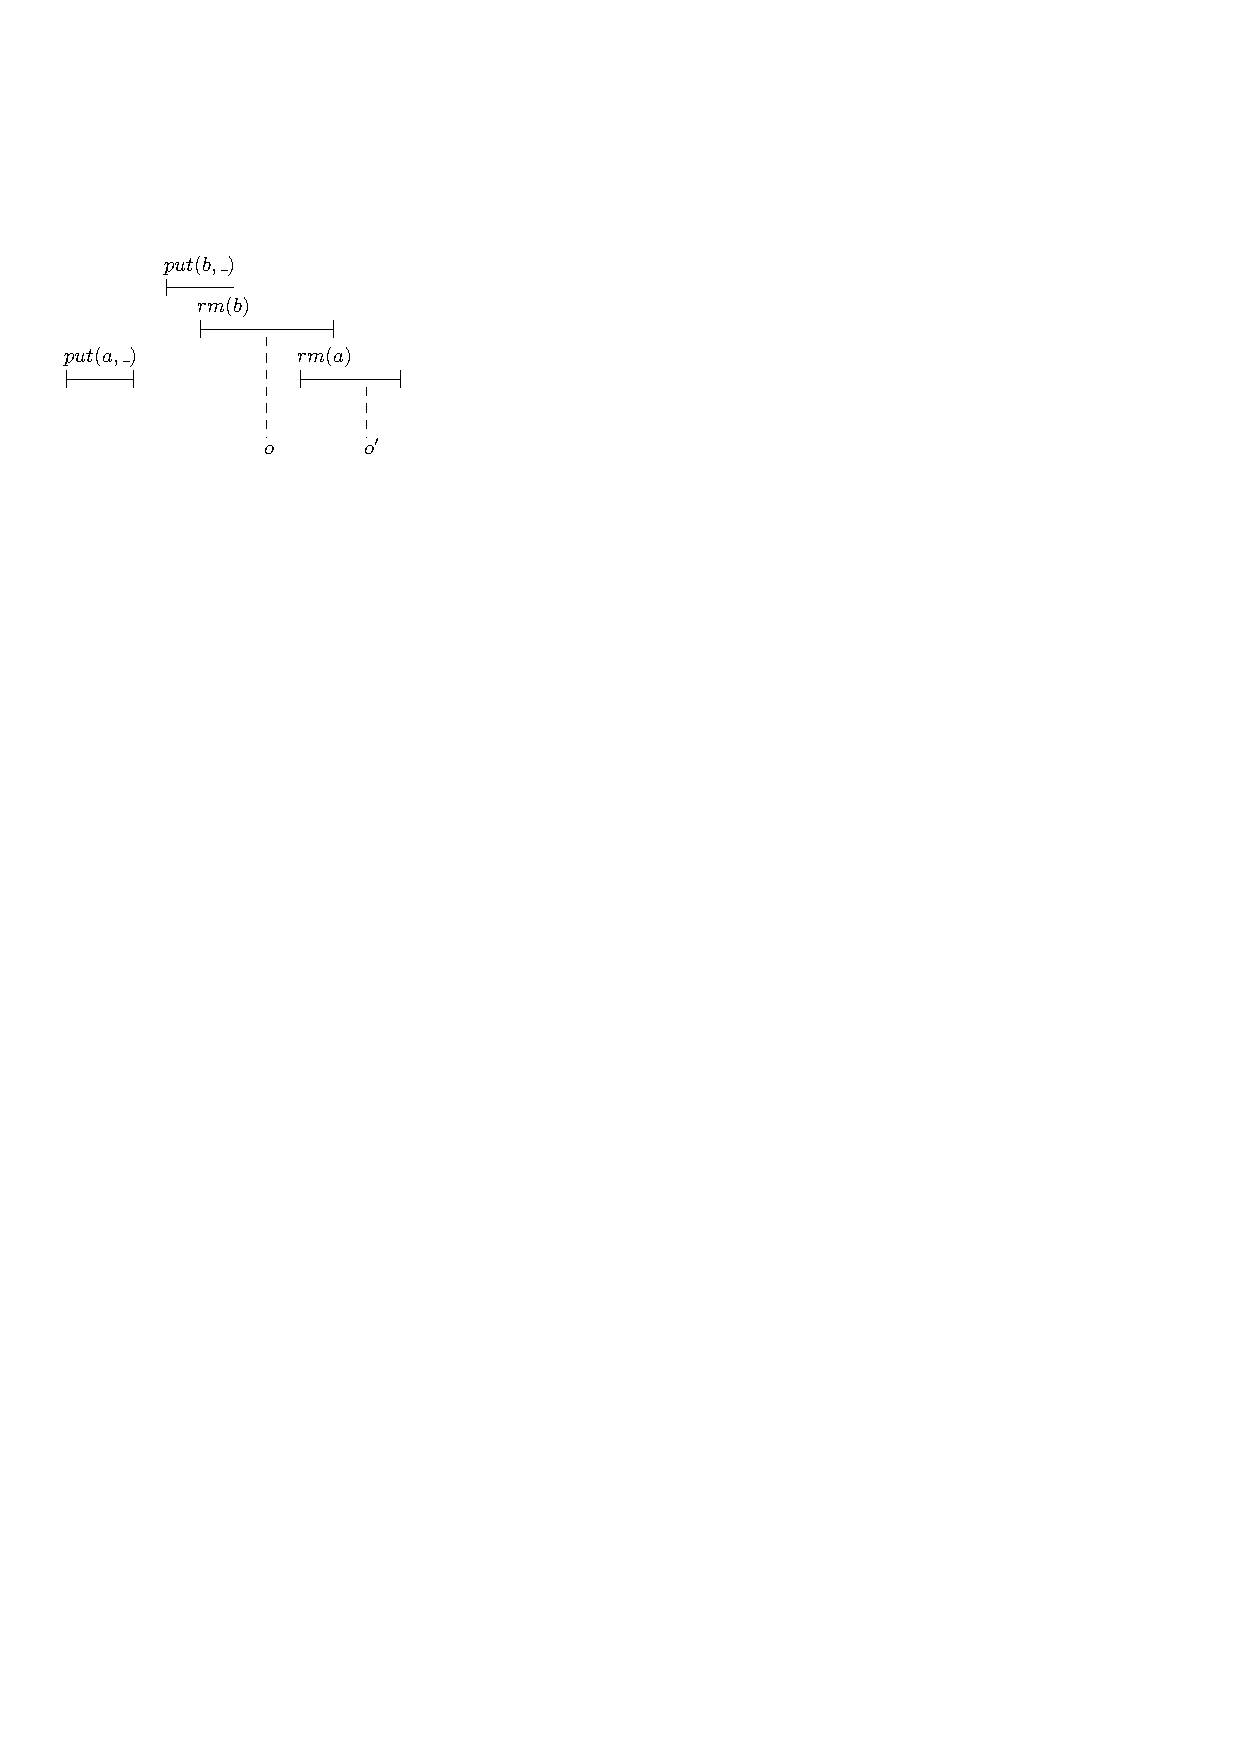
\includegraphics[width=0.4 \textwidth]{PIC-HIS-Apr2-A-1.pdf}
%\vspace{-10pt}
  \caption{The first possible enumeration.}
  \label{fig:history enumeration 1 for Rpr2}
\end{figure}


\begin{figure}[htbp]
  \centering
  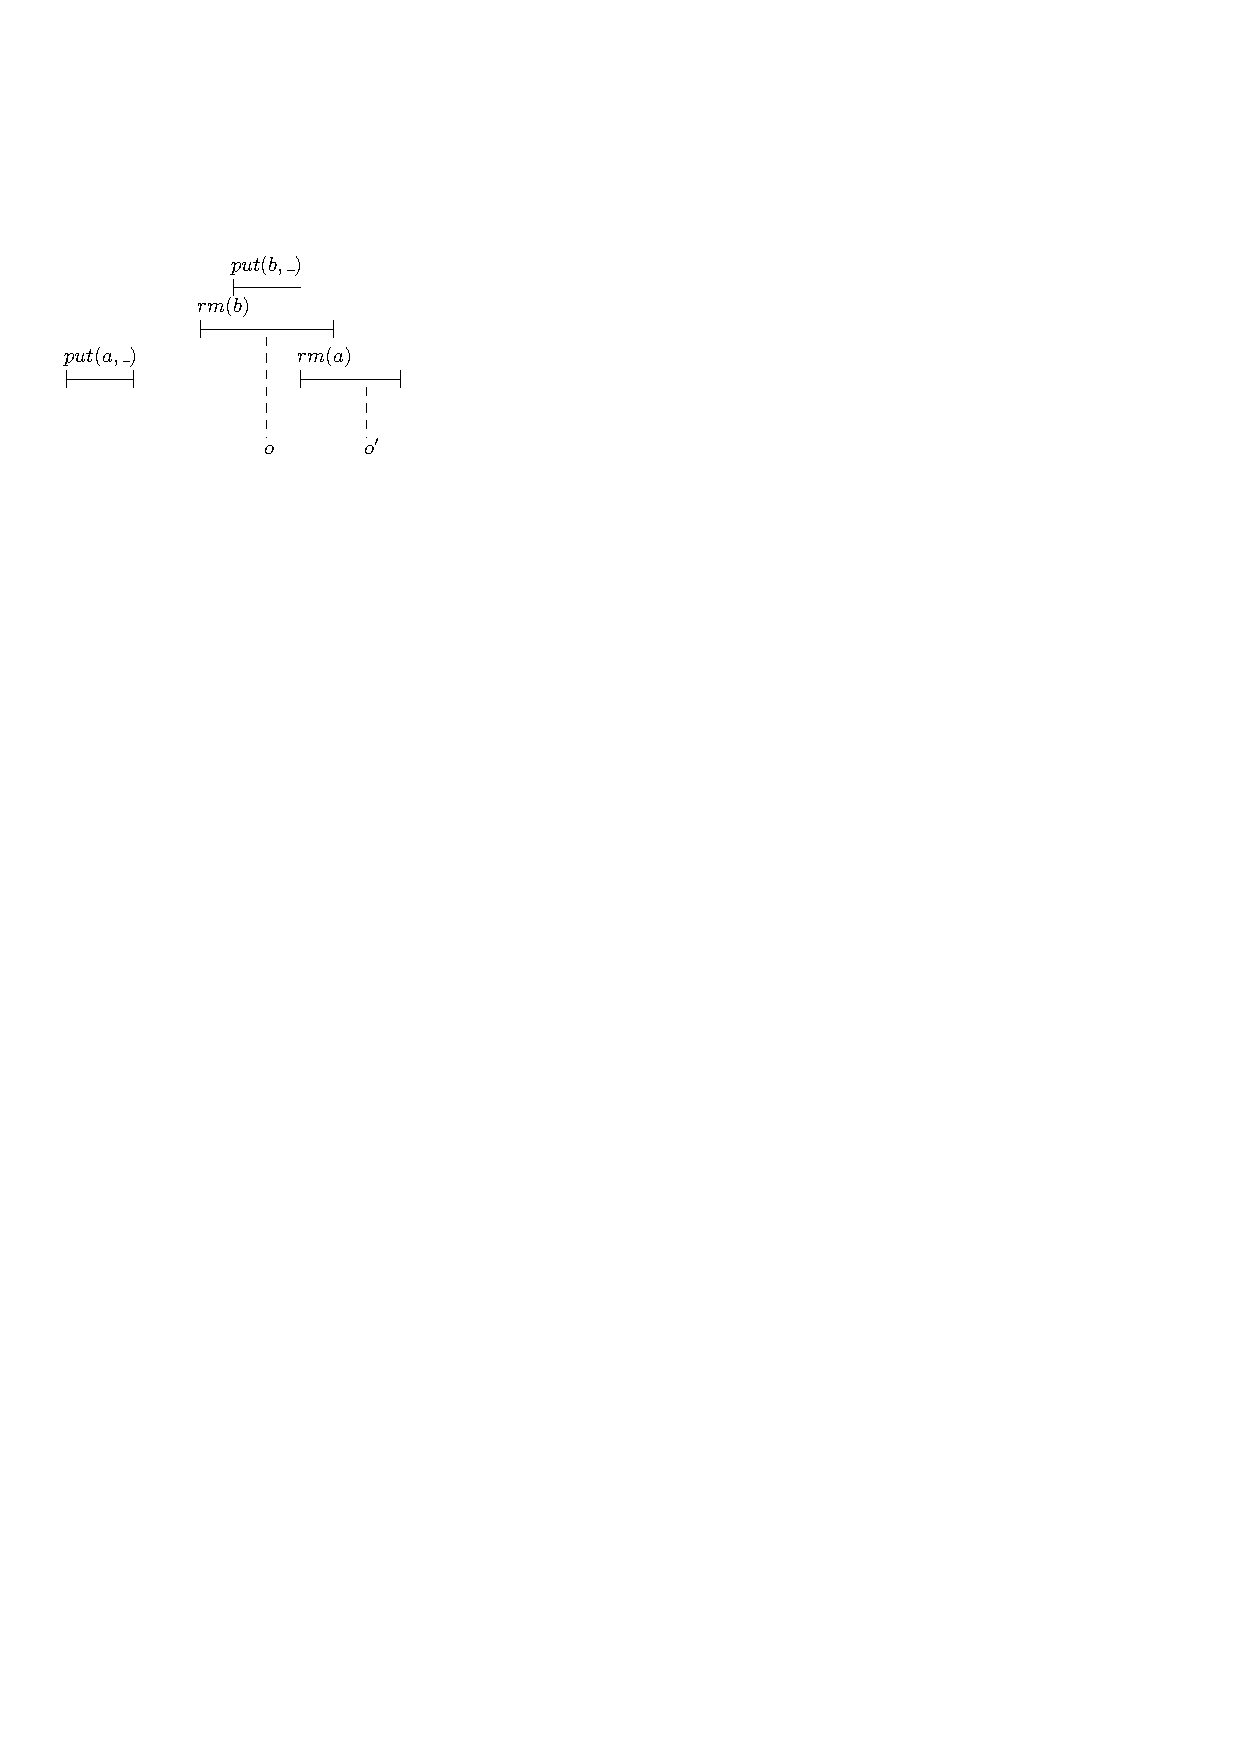
\includegraphics[width=0.4 \textwidth]{PIC-HIS-Apr2-A-2.pdf}
%\vspace{-10pt}
  \caption{The second possible enumeration.}
  \label{fig:history enumeration 2 for Rpr2}
\end{figure}

\begin{figure}[htbp]
  \centering
  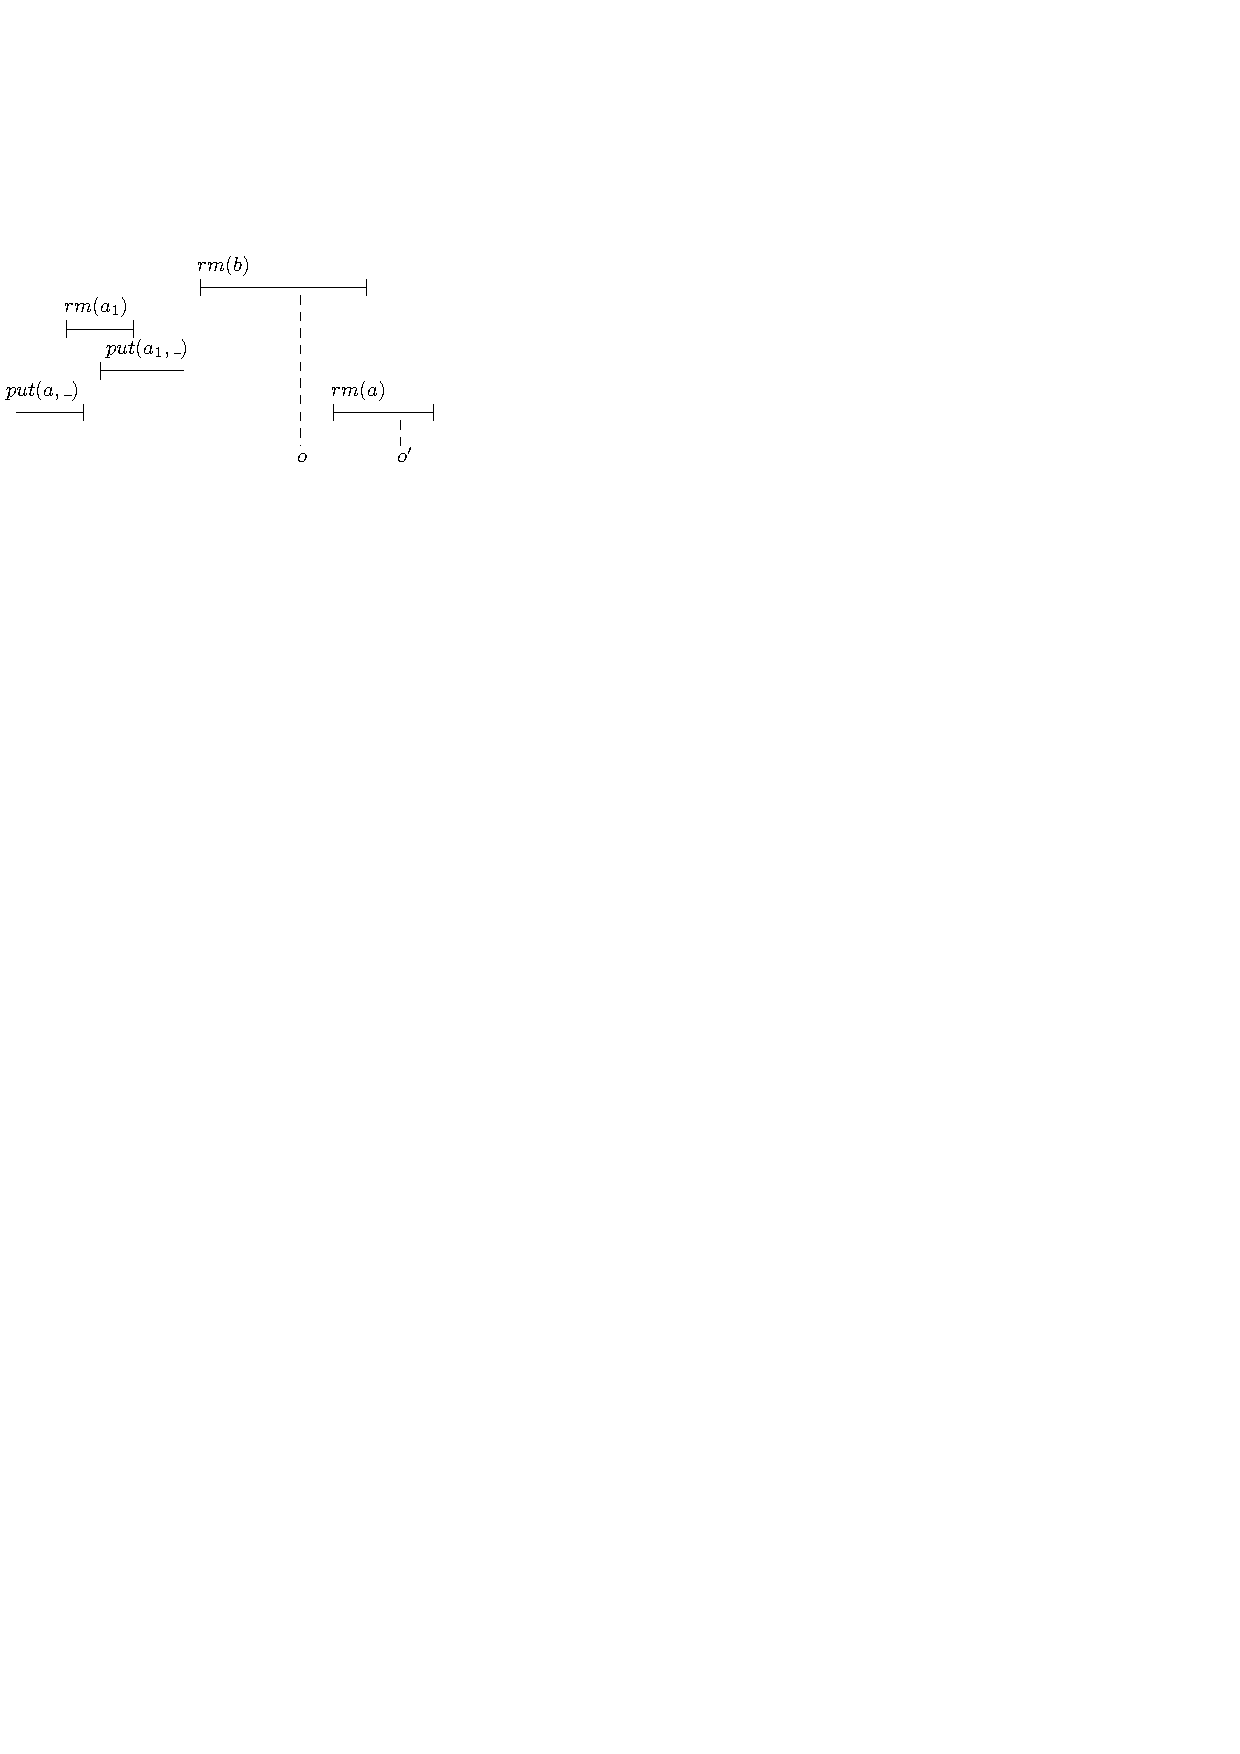
\includegraphics[width=0.4 \textwidth]{PIC-HIS-Apr2-A-3.pdf}
%\vspace{-10pt}
  \caption{The third possible enumeration.}
  \label{fig:history enumeration 3 for Rpr2}
\end{figure}

\begin{figure}[htbp]
  \centering
  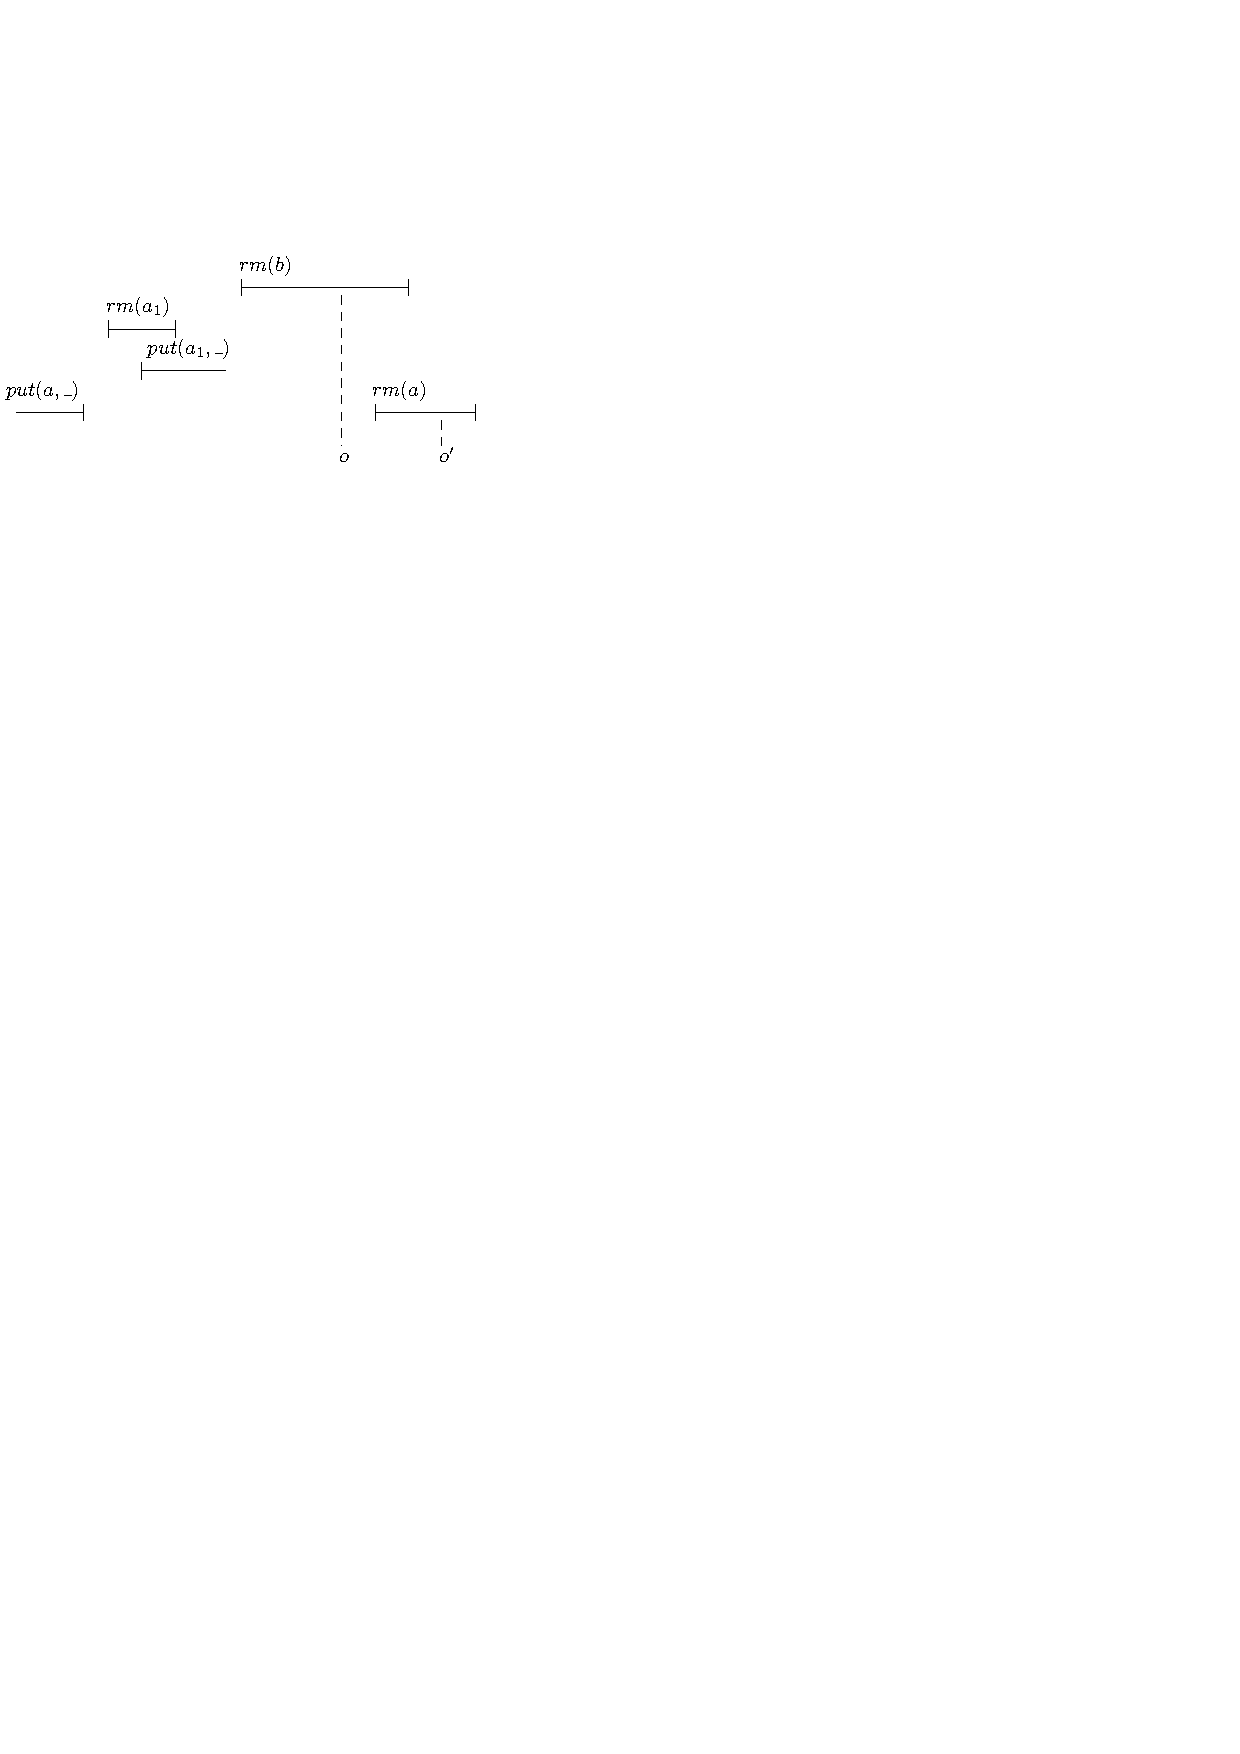
\includegraphics[width=0.4 \textwidth]{PIC-HIS-Apr2-A-4.pdf}
%\vspace{-10pt}
  \caption{The forth possible enumeration.}
  \label{fig:history enumeration 4 for Rpr2}
\end{figure}

\begin{figure}[htbp]
  \centering
  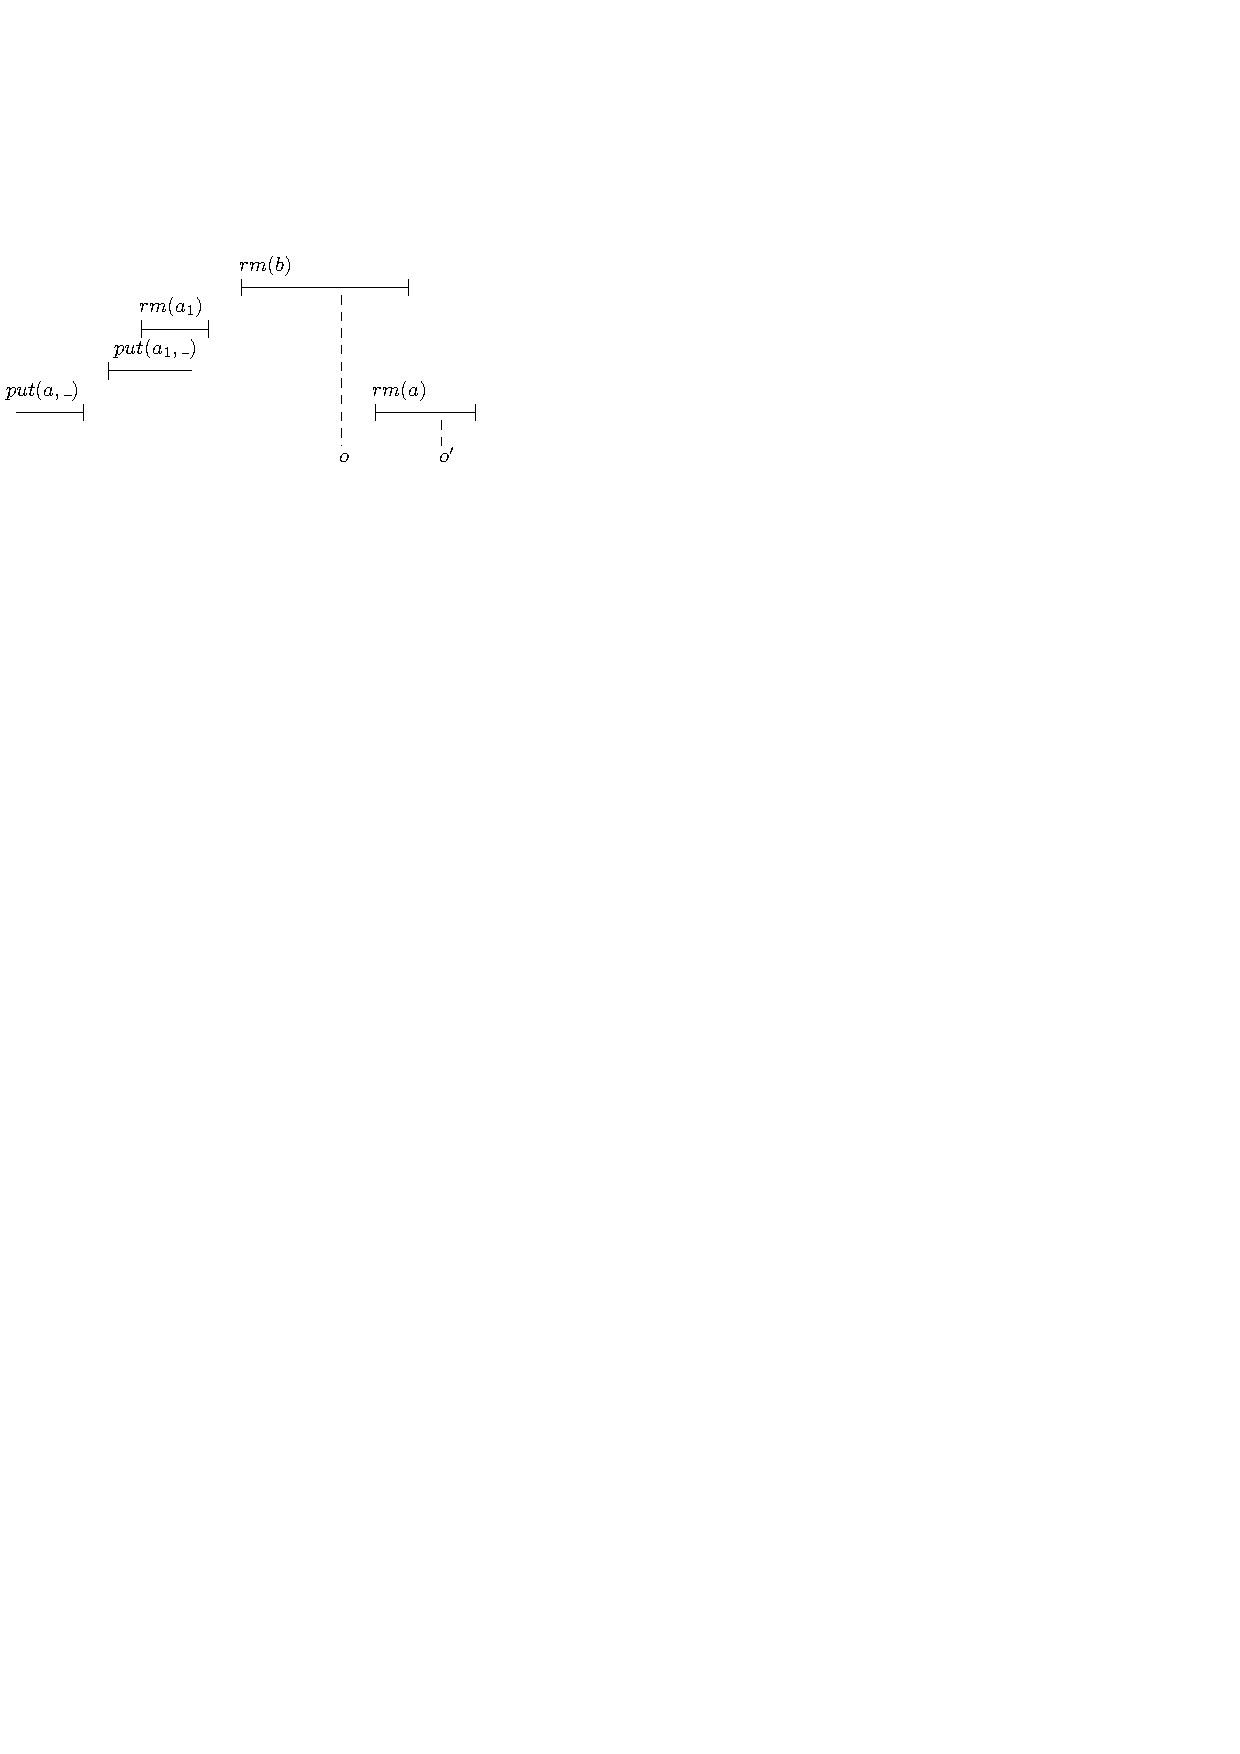
\includegraphics[width=0.4 \textwidth]{PIC-HIS-Apr2-A-5.pdf}
%\vspace{-10pt}
  \caption{The fifth possible enumeration.}
  \label{fig:history enumeration 5 for Rpr2}
\end{figure}

Given a data-differentiated history $h$, two actions $\textit{act}_1$, $\textit{act}_2$ of items of priority $\textit{pri}$, and assume that $\textit{act}_1$ is before $\textit{act}_2$ in $h$. We say that $\textit{act}_1$, $\textit{act}_2$ is covered by items $d_1,\ldots,d_m$ in $h$, if the priorities of $d_1,\ldots,d_m$ is not $\textit{pri}$, and

\begin{itemize}
\setlength{\itemsep}{0.5pt}
\item[-] $\textit{ret}(\textit{put},d_m,\_)$ is before $\textit{act}_1$,

\item[-] For each $i < 1 \leq m$,$\textit{put}(d_{\textit{i-1}},\_)$ happens before $\textit{rm}(d_i)$,

\item[-] $\textit{act}_2$ is before $\textit{cal}(\textit{rm},d_1)$.
\end{itemize}

According to the definition of gap-point, in \figurename~\ref{fig:history enumeration 1 for Rpr2}, \figurename~\ref{fig:history enumeration 2 for Rpr2}, \figurename~\ref{fig:history enumeration 3 for Rpr2}, \figurename~\ref{fig:history enumeration 4 for Rpr2} or \figurename~\ref{fig:history enumeration 5 for Rpr2}, the location of $o$ and $o'$ is equivalent to that, there exists items $d_1,\ldots,d_m$ in $h$ in $h$, such that $\textit{cal}(\textit{rm},a)$ and $\textit{ret}(\textit{rm},b)$ is covered by $d_1,\ldots,d_m$, $\textit{cal}(\textit{rm},b)$ is before $\textit{ret}(\textit{put},d_m,\_)$ in $h$, and $\textit{cal}(\textit{rm},d_1)$ is before $\textit{ret}(\textit{rm},a)$ in $h$. We say that such $d_1,\ldots,d_m$ constitute the rightmost gap of $\textit{put}(b,\_)$ and $\textit{rm}(b)$.

An automaton $\mathcal{A}_{\textit{Rpr2-1}}$ is given in \figurename~\ref{fig:automata for first enumeration of Rpr2}, and it is constructed for the first enumeration in \figurename~\ref{fig:history enumeration 1 for Rpr2}. In \figurename~\ref{fig:automata for first enumeration of Rpr2}, we renames the items that covers $\textit{cal}(\textit{rm},a)$ and $\textit{ret}(\textit{rm},b)$ into $d$, and rename the renaming items into $e$. Here let $c = \textit{cal}(\textit{put},e,\textit{anyPri}),\textit{ret}(\textit{put},e)$, $\textit{cal}(\textit{rm},e), \textit{ret}(\textit{rm},e)$, $c_1 = c + \textit{cal}(\textit{put},d,\textit{les}_p)$, $c_2 = c_1 + \textit{ret}(\textit{put},b)$, $c_3 = c_2 + \textit{ret}(\textit{rm},d)$, $c_4 = c + \textit{ret}(\textit{put},b) + \textit{ret}(\textit{rm},d)$.

\begin{figure}[htbp]
  \centering
  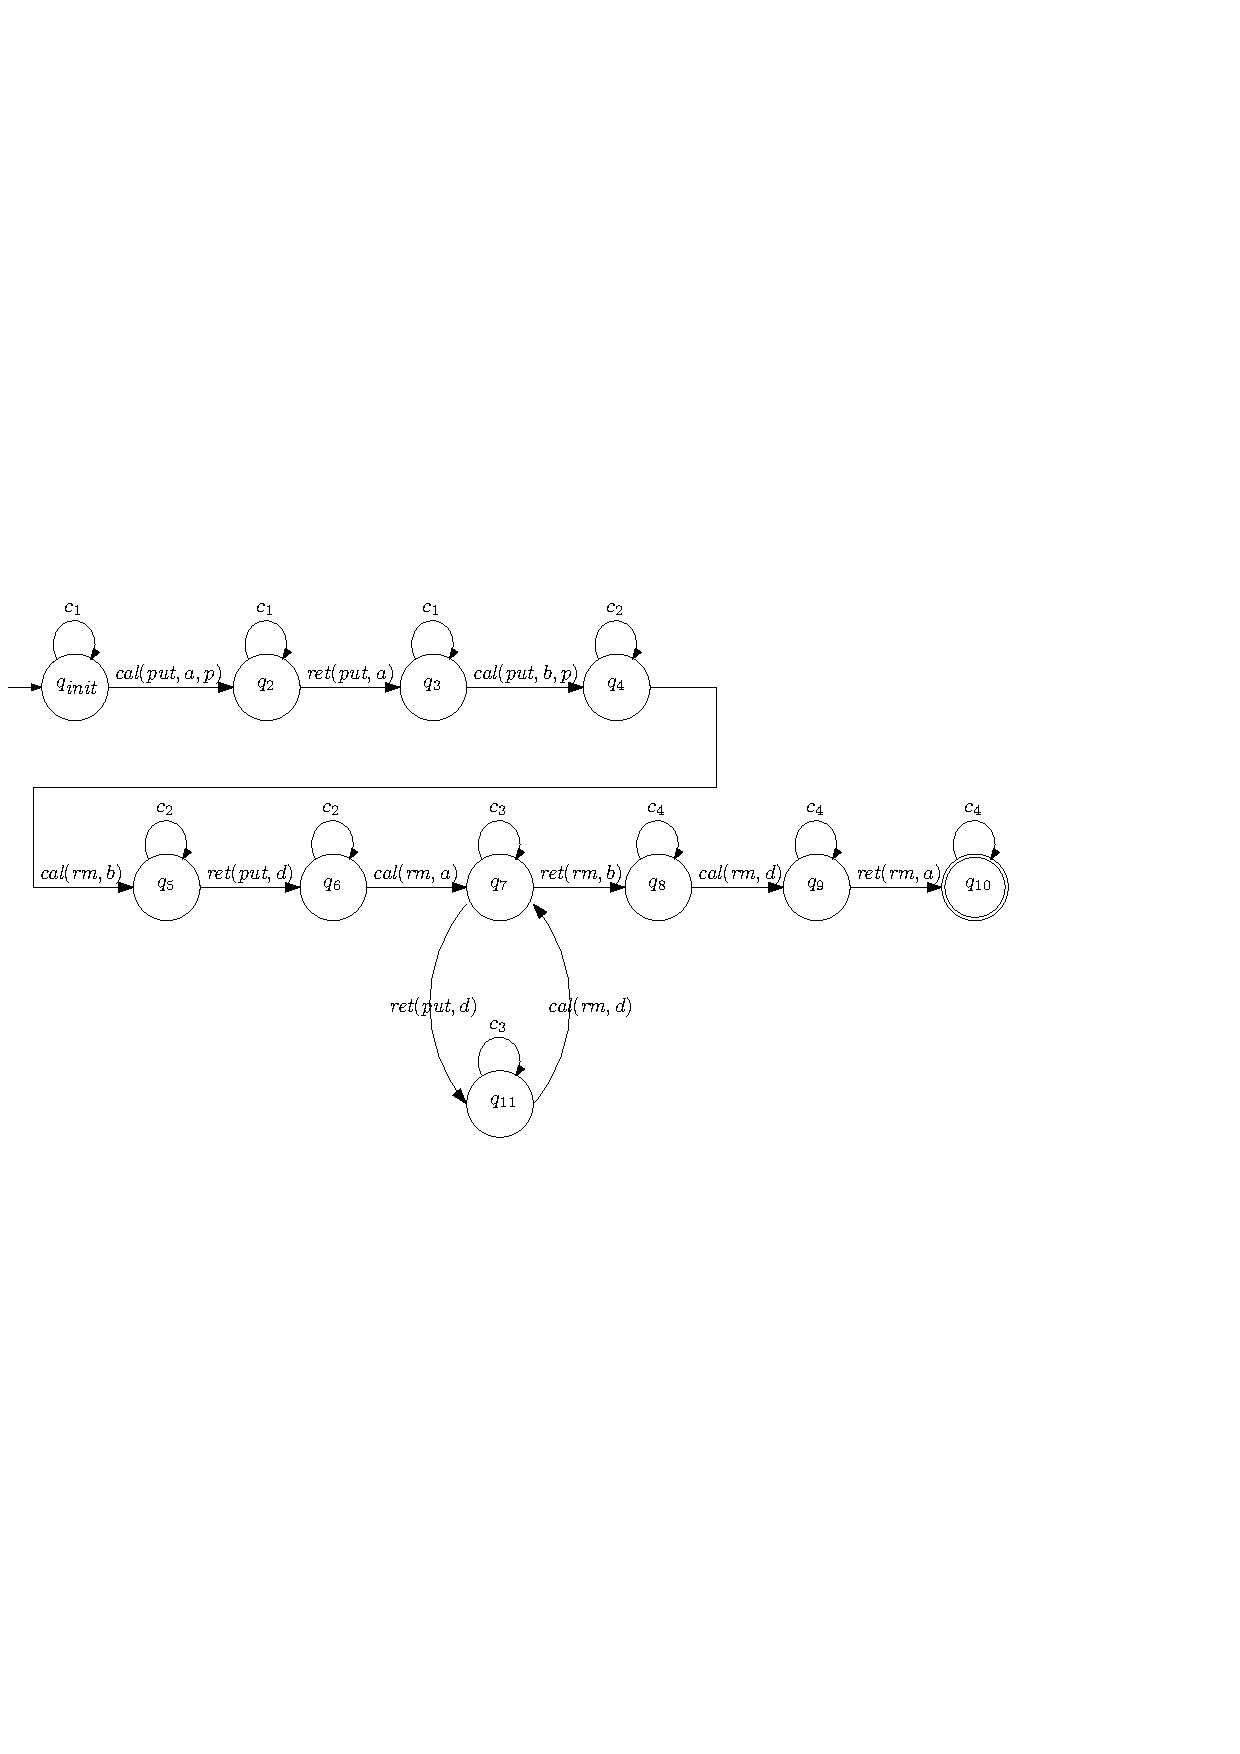
\includegraphics[width=0.8 \textwidth]{PIC_AUTO_Rpr2_1.pdf}
%\vspace{-10pt}
  \caption{Automaton $\mathcal{A}_{\textit{Rpr2-1}}$}
  \label{fig:automata for first enumeration of Rpr2}
\end{figure}


An automaton $\mathcal{A}_{\textit{Rpr2-2}}$ is given in \figurename~\ref{fig:automata for second enumeration of Rpr2}, and it is constructed for the second enumeration in \figurename~\ref{fig:history enumeration 2 for Rpr2}. In \figurename~\ref{fig:automata for second enumeration of Rpr2}, $c_1$, $c_2$, $c_3$ and $c_4$ is same as that in \figurename~\ref{fig:automata for first enumeration of Rpr2}.

\begin{figure}[htbp]
  \centering
  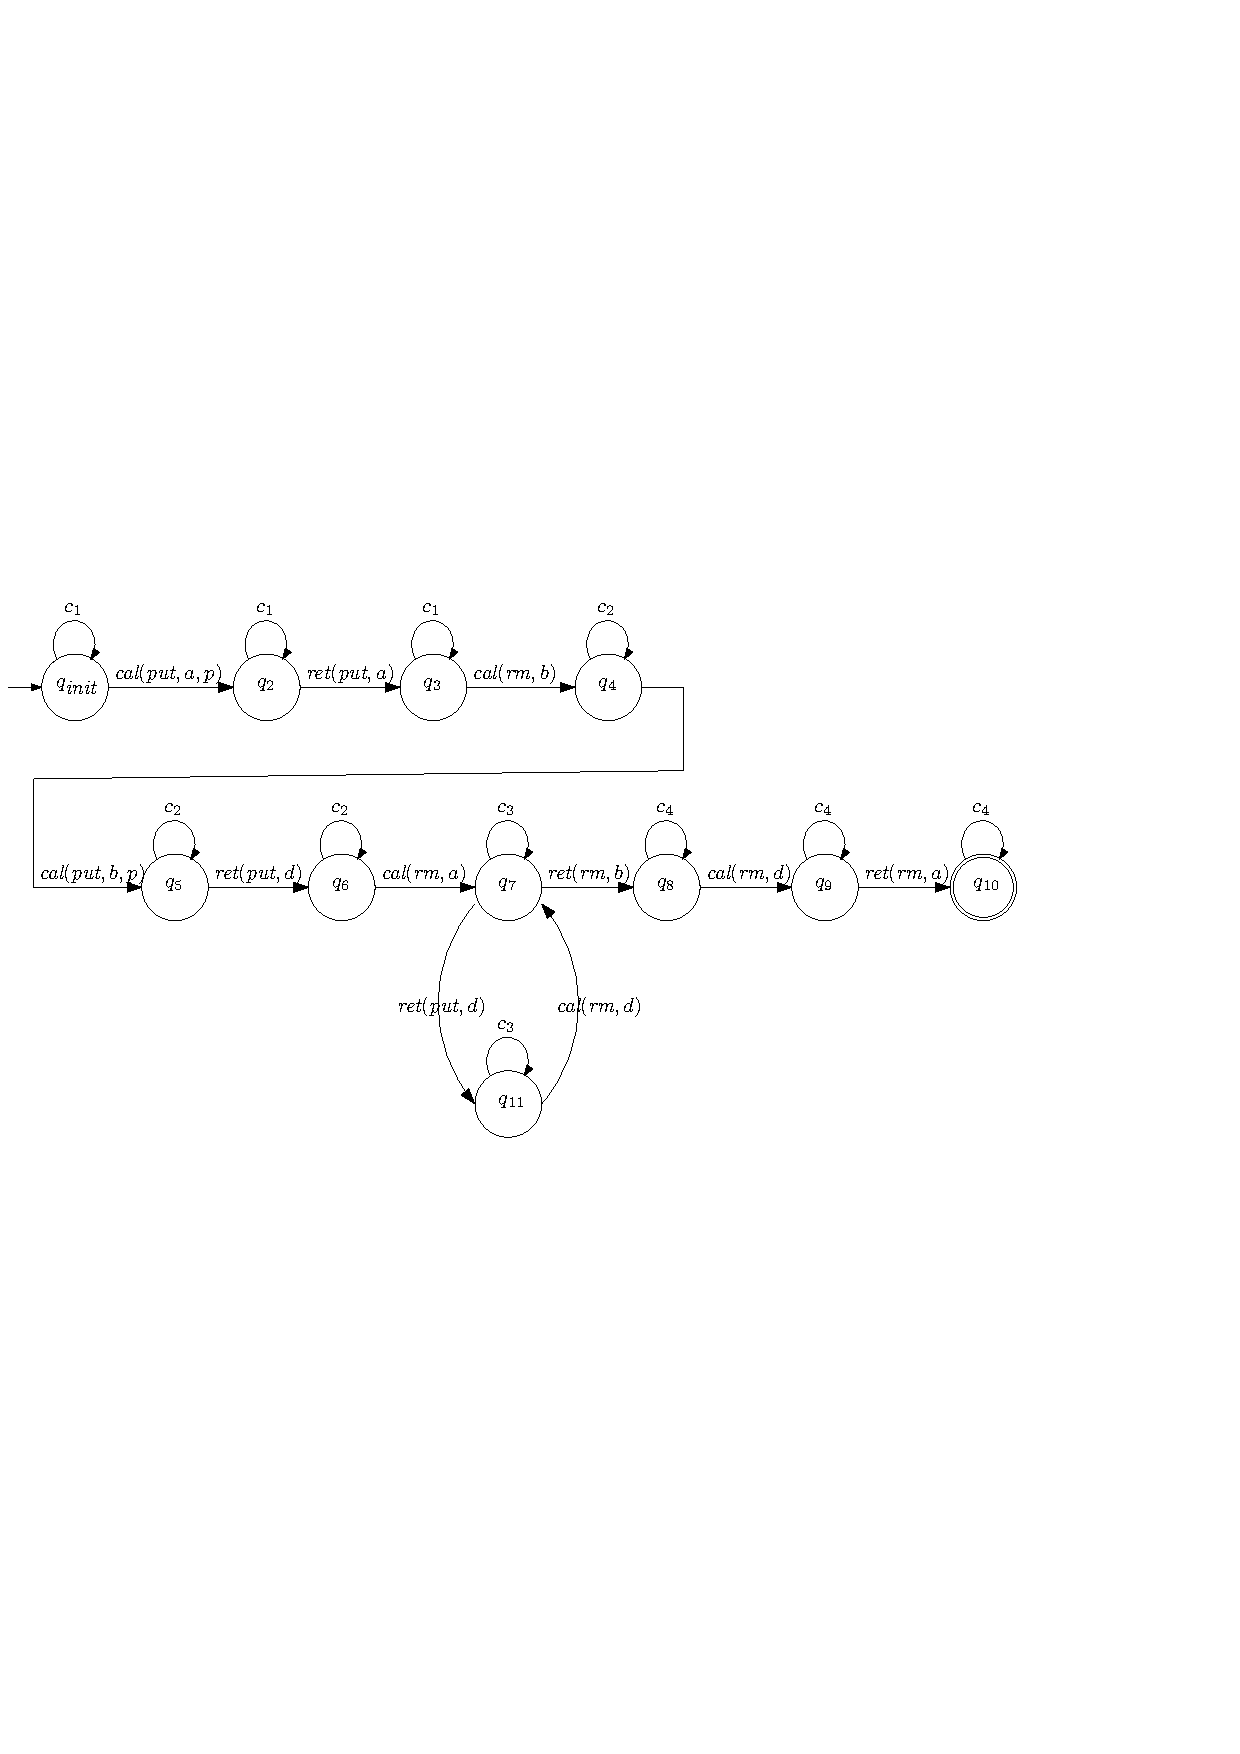
\includegraphics[width=0.8 \textwidth]{PIC_AUTO_Rpr2_2.pdf}
%\vspace{-10pt}
  \caption{Automaton $\mathcal{A}_{\textit{Rpr2-2}}$}
  \label{fig:automata for second enumeration of Rpr2}
\end{figure}

For the third enumeration in \figurename~\ref{fig:history enumeration 3 for Rpr2}. Since we want to ensure that $a$ and $b$ are putted only once, we need to explicitly record the positions of $\textit{cal}(\textit{put},a,p)$ and $\textit{cal}(\textit{put},b,p)$. Since the positions of $\textit{cal}(\textit{put},a,p)$ and $\textit{cal}(\textit{put},b,p)$ are not fixed, there are finite possible cases to consider, as shown below:

\begin{itemize}
\setlength{\itemsep}{0.5pt}
\item[-] If $\textit{cal}(\textit{put},b,p)$ is after $\textit{cal}(\textit{rm},b)$ and before $\textit{cal}(\textit{rm},a)$: There are two possible positions of $\textit{cal}(\textit{put},a,p)$: (1) before $\textit{cal}(\textit{rm},a_1)$, and (2) after $\textit{cal}(\textit{rm},a_1)$, and before $\textit{ret}(\textit{put},a)$.

\item[-] If $\textit{cal}(\textit{put},b,p)$ is after $\textit{ret}(\textit{rm},a_1)$ and before $\textit{cal}(\textit{rm},b)$: same as above case.

\item[-] If $\textit{cal}(\textit{put},b,p)$ is after $\textit{cal}(\textit{put},a_1,\_)$ and before $\textit{ret}(\textit{rm},a_1)$: same as above case.

\item[-] If $\textit{cal}(\textit{put},b,p)$ is after $\textit{ret}(\textit{put},a)$ and before $\textit{cal}(\textit{put},a_1,p)$: same as above case.

\item[-] If $\textit{cal}(\textit{put},b,p)$ is after $\textit{cal}(\textit{rm},a_1)$ and before $\textit{ret}(\textit{put},a)$: There are three possible positions of $\textit{cal}(\textit{put},a,p)$: (1) after $\textit{cal}(\textit{put},b,p)$ and before $\textit{ret}(\textit{put},a)$, (2) after $\textit{cal}(\textit{rm},a_1)$ and before $\textit{cal}(\textit{put}b,p)$, and (3) before $\textit{call}(\textit{rm},a_1)$.

\item[-] If $\textit{cal}(\textit{put},b,p)$ is before $\textit{cal}(\textit{rm},a_1)$: There are three possible positions of $\textit{cal}(\textit{put},a,p)$: (1) after $\textit{cal}(\textit{rm},a_1)$ and before $\textit{ret}(\textit{put},a)$, (2) after $\textit{cal}(\textit{put},b,p)$ and before $\textit{cal}(\textit{rm},a_1)$, and (3) before $\textit{cal}(\textit{put},b,p)$.
\end{itemize}

Therefore, there are fourteen possible cases that satisfy the third enumeration in \figurename~\ref{fig:history enumeration 3 for Rpr2}. For each case, we construct an finite automaton. Let $\textit{Aut}_{\textit{Rpr2-3}}$ be the set of finite automata that is constructed for above fourteen cases. For example, for the case $\textit{ca}_1$ when $\textit{cal}(\textit{put},a,p)$ is before $\textit{cal}(\textit{rm},a_1)$, $\textit{cal}(\textit{put},b,p)$ is after $\textit{ret}(\textit{rm},a_1)$, and $\textit{cal}(\textit{put},b,p)$ is before $\textit{cal}(\textit{rm},b)$, we construct a finite automaton in \figurename~\ref{fig:automata for ca1 of third enumeration of Rpr2}. In \figurename~\ref{fig:automata for ca1 of third enumeration of Rpr2}, let $c$ and $c_1 = c + \textit{cal}(\textit{put},d,\textit{les}_p)$ the same as that in \figurename~\ref{fig:automata for first enumeration of Rpr2}. Let $c_2 = c_1 + \textit{ret}(\textit{put},a_1)$, $c_3 = c_2 + \textit{ret}(\textit{put},b)$, $c_4 = c_3 + \textit{ret}(\textit{rm},d)$, and $c_5 = c + \textit{ret}(\textit{put},b) + \textit{ret}(\textit{put},a_1) + \textit{ret}(\textit{rm},d)$. The other finite automata in $\textit{Aut}_{\textit{Rpr2-3}}$ can be similarly constructed.

\begin{figure}[htbp]
  \centering
  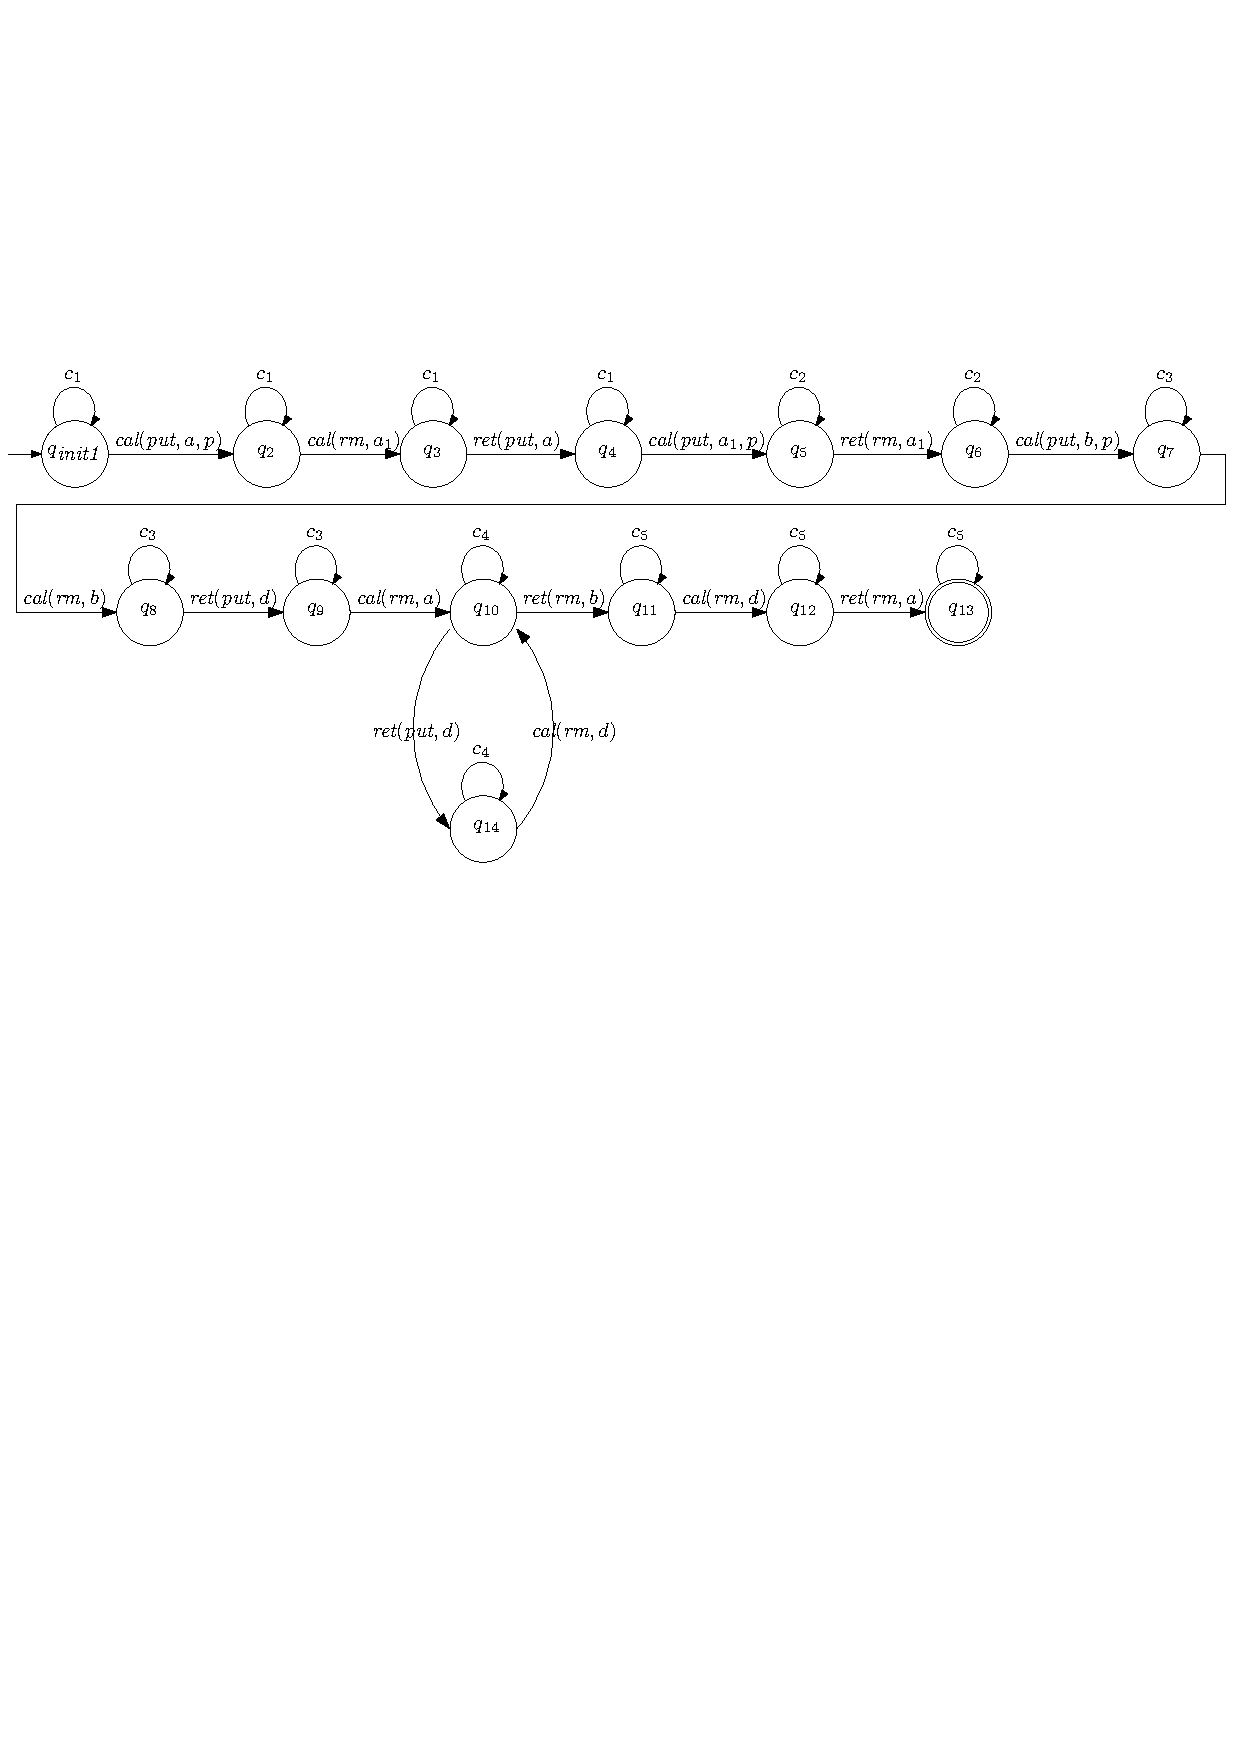
\includegraphics[width=0.8 \textwidth]{PIC_AUTO_Rpr2_3.pdf}
%\vspace{-10pt}
  \caption{Automaton for $\textit{ca}_1$}
  \label{fig:automata for ca1 of third enumeration of Rpr2}
\end{figure}

Similarly, we construct sets $\textit{Aut}_{\textit{Rpr2-4}}$ and $\textit{Aut}_{\textit{Rpr2-5}}$ of finite automata for the forth enumeration in \figurename~\ref{fig:history enumeration 4 for Rpr2} and the fifth enumeration in \figurename~\ref{fig:history enumeration 5 for Rpr2}, respectively.


\begin{restatable}{lemma}{Rpr2IsCoRegular}
\label{lemma:Rpr2 is co-regular}
$R_{\textit{pr2}}$ is co-regular.
\end{restatable}

\begin {proof}

Let $\textit{AutS-R}_{\textit{pr2}} = \{ \mathcal{A}_{\textit{Rpr2-1}}, \mathcal{A}_{\textit{Rpr2-2}} \} \cup \textit{Aut}_{\textit{Rpr2-3}} \cup \textit{Aut}_{\textit{Rpr2-4}} \cup \textit{Aut}_{\textit{Rpr2-5}}$. We need to prove that:

\noindent {\bf $\textit{fact}_1$}: Given a data-independent implementation $\mathcal{I}$, $\textit{AutS-R}_{\textit{pr2}} \cap \mathcal{I} \neq \emptyset$, if and only if there exists data-differentiated history $h \in \mathcal{I}$, $h'$ is a projection of $h$, $\textit{last}(h') = R_{\textit{pr2}}$ and $h$ does not linearizable to $\textit{MR}_{\textit{pr2}}$.

By Lemma \ref{lemma:Rpr2 as gap-point and ob order}, $\textit{fact}_1$ is equivalent to $\textit{fact}_2$:

\noindent {\bf $\textit{fact}_2$}: Given a data-independent implementation $\mathcal{I}$, $\textit{AutS-R}_{\textit{pr0}} \cap \mathcal{I} \neq \emptyset$, if and only if there exists data-differentiated history $h \in \mathcal{I}$, $h'$ is a projection of $h$, such that $\textit{last}(h') = R_{\textit{pr2}}$, $a$ and $b$ has maximal priority in $h'$, $a <_{\textit{ob}} b$ in $h'$, and the rightmost gap-point of $\textit{put}(b,\_)$ and $\textit{rm}(b)$ is before $\textit{cal}(\textit{put},a,\_)$ or $\textit{cal}(\textit{rm},a)$ in $h''$.

\noindent The $\textit{only if}$ direction: Assume that $h_1 \in \mathcal{I}$ is accepted by $\textit{AutS-R}_{\textit{pr2}}$. By data-independence, there exists data-differentiated sequence $h_2 \in \mathcal{I}$ and a renaming function $r$, such that $h_1=r(h_2)$. Since $h_1$ is accepted by $\textit{AutS-R}_{\textit{pr2}}$, let $x$ and $y$ be the items that are renamed into $b$ and $a$ by $r$, respectively, and let $d_1,\ldots,d_m$ be the items that are renamed into $d$ by $r$.

let $h'' = h_2 \vert_{ \{ x,y,d_1,\ldots,d_m \} }$. It is obvious that $\textit{last}(h'') = R_{\textit{pr2}}$. According to our construction of automata in $\textit{AutS-R}_{\textit{pr2}}$, it is not hard to see that $x$ and $y$ has maximal priority in $h_2$, $y <_{\textit{ob}} x$ in $h''$, and the rightmost gap-point of $\textit{put}(x,\_)$ and $\textit{rm}(x)$ is before $\textit{cal}(\textit{put},y,\_)$ or $\textit{cal}(\textit{rm},y)$ in $h''$. %By Lemma \ref{lemma:Rpr2 as gap-point and ob order}, we know that $h''$ is not linearizable to $\textit{MR}_{\textit{pr2}}$.

\noindent The $\textit{if}$ direction: Assume that there exists $h' \in \textit{proj}(h)$, such that $\textit{last}(h') = R_{\textit{pr2}}$, $a'$ and $b'$ has maximal priority in $h'$, $a' <_{\textit{ob}} b'$ in $h'$, and the rightmost gap-point of $\textit{put}(b',\_)$ and $\textit{rm}(b')$ is before $\textit{cal}(\textit{put},a',\_)$ or $\textit{cal}(\textit{rm},a')$ in $h''$. By data-independence, we can obtain history $h_1$ as follows: (1) rename $a'$ and $b'$ into $a$ and $b$, respectively, (2) for the items $d_1,\ldots,d_m$ that constitute the rightmost gap of $\textit{put}(x,\_)$ and $\textit{rm}(x)$, we rename them into $d$, and (3) rename the other items into $e$. It is easy to see that $\textit{last}(h_1) = R_{\textit{pr2}}$, $a$ and $b$ has maximal priority in $h_1$, $a <_{\textit{ob}} b$ in $h_1$, and the rightmost gap-point of $\textit{put}(b,\_)$ and $\textit{rm}(b)$ is before $\textit{cal}(\textit{put},a,\_)$ or $\textit{cal}(\textit{rm},a)$ in $h''$. By Lemma \ref{lemma:five enumeration is enough for Rpr2}, there are five possible enumeration of operations of $a$, $b$, $a_1$ (if exists) and $a_2$ (if exists). Then


\begin{itemize}
\setlength{\itemsep}{0.5pt}
\item[-] If $a <_{\textit{ob}} b$ because of the first enumeration, it is easy to see that $h_1$ is accepted by $\mathcal{A}_{\textit{Rpr2-1}}$.

\item[-] If $a <_{\textit{ob}} b$ because of the second enumeration, it is easy to see that $h_1$ is accepted by $\mathcal{A}_{\textit{Rpr2-2}}$.

\item[-] If $a <_{\textit{ob}} b$ because of the third enumeration, it is easy to see that $h_1$ is accepted by some automaton in $\textit{Aut}_{\textit{Rpr2-3}}$.

\item[-] If $a <_{\textit{ob}} b$ because of the forth enumeration, it is easy to see that $h_1$ is accepted by some automaton in $\textit{Aut}_{\textit{Rpr2-4}}$.

\item[-] If $a <_{\textit{ob}} b$ because of the fifth enumeration, it is easy to see that $h_1$ is accepted by some automaton in $\textit{Aut}_{\textit{Rpr2-5}}$.
\end{itemize}

This completes the proof of this lemma. \qed
\end {proof}



\subsection{Co-Regular of $R_{\textit{pr3}}$}
\label{subsec:co-regular of Rpr3}


\begin{restatable}{lemma}{Rpr3IsAlwaysCoRegular}
\label{lemma:Rpr3 is always co-regular}
Given a data-differentiated history $h$, if $\textit{last}(h) = R_{\textit{pr3}}$, then $h \sqsubseteq \textit{MR}_{\textit{pr3}}$.
\end{restatable}

\begin {proof}

Since $\textit{last}(h) = R_{\textit{pr3}}$, there exists item $x$ with $\textit{pri}_x$ in $h$, such that $h \vert_{ \{ x \}} = \textit{put}(x,\textit{pri}_x)$, and $\textit{pri}_x$ is larger than any priority of $h$.

For each operation, we locate its linearization point just after its call action. In such way we obtain a sequence $l$ of operations, and it is easy to see that $h \sqsubseteq l$. It is obvious that $l$ contains $\textit{put}(x,\textit{pri})$, and then $l \in \textit{MR}_{\textit{pr3}}$. This completes the proof of this lemma. \qed
\end {proof}



\subsection{Co-Regular of $R_{\textit{pr4}}$}
\label{subsec:co-regular of Rpr4}

\begin{restatable}{lemma}{Rp4AsHappenBefore}
\label{lemma:Rpr4 as happen before}
Given a data-differentiated history $h$. There exists $h' \in \textit{proj}(h)$, such that $\textit{last}(h') = R_{\textit{pr4}}$, and $h'$ does not linearizable to $\textit{MR}_{\textit{pr4}}$, if and only if there exists $h'' \in \textit{proj}(h)$, $\textit{last}(h'') = R_{\textit{pr4}}$, $x$ and $y$ has maximal priority in $h''$, $x$ has unmatched $\textit{put}$, $y$ has matched $\textit{put}$ and $\textit{rm}$, and $\textit{put}(x,\_) <_{\textit{hb}} \textit{put}(y,\_)$.
\end{restatable}

\begin {proof}

To prove the $\textit{if}$ direction, let $h_1 = h \vert_{ \{ x,y \} }$. It is easy to see that $\textit{last}(h') = R_{\textit{pr4}}$ and $h_1$ does not linearizable to $\textit{MR}_{\textit{pr4}}$.

To prove the $\textit{only if}$ direction, we prove its contrapositive. Assume that for each $h'' \in \textit{proj}(h)$, such that $\textit{last}(h'') = R_{\textit{pr4}}$, for each $x$ and $y$ has maximal priority in $h''$, if $x$ has unmatched $\textit{put}$, $y$ has matched $\textit{put}$ and $\textit{rm}$, then $\textit{put}(x,\_)$ does not happen before $\textit{put}(y,\_)$. We need to prove that, for each $h' \in \textit{proj}(h)$, if $\textit{last}(h') = R_{\textit{pr4}}$, then $h' \sqsubseteq \textit{MR}_{\textit{pr4}}$.

Given such $h'$, let $x_1,\ldots,x_m$ be the set of items with maximal priority and has unmatched $\textit{put}$ operations, let $y_1,\ldots,y_n$ be the set of items with maximal priority and has matched $\textit{put}$ and $\textit{rm}$ operations. It is easy to see that, for each $x_i$ and $y_j$, $\textit{cal}(\textit{put},y_j)$ is before $\textit{ret}(\textit{put},x_i,\_)$. Then we locate the linearization points of $h'$ as follows:

\begin{itemize}
\setlength{\itemsep}{0.5pt}
\item[-] For each $x_i$, locate the linearization point of $\textit{put}(x_i,\_)$ just before its return action.

\item[-] For each $y_j$, locate the lineariztion point of $\textit{put}(y_j,\_)$ jest after its call action.

\item[-] For other operations, locate their linearization points at an arbitrary location after its call action and before its return action.
\end{itemize}

Let $l$ be the sequence of linearization points. It is easy to see that $h \sqsubseteq l$, and $l \in \textit{MR}_{\textit{pr4}}$. Here the $\textit{itm}$ in $R_{\textit{pr4}}$ is chosen to be $\textit{ret}(\textit{put},x_{\textit{ind}},\_)$, where the return action of $x_{\textit{ind}}$ is later than return actions of other $x_i$. This completes the proof of this lemma. \qed
\end {proof}


\begin{restatable}{lemma}{Rpr4IsAlwaysCoRegular}
\label{lemma:Rpr4 is always co-regular}
Given a data-differentiated history $h$, if $\textit{last}(h) = R_{\textit{pr4}}$, then $h \sqsubseteq \textit{MR}_{\textit{pr4}}$.
\end{restatable}

\begin {proof}

According to Lemma \ref{lemma:Rpr4 as happen before}, if $\textit{last}(h) = R_{\textit{pr4}}$ and $h$ does not linearizable to $\textit{MR}_{\textit{pr4}}$, then there exists $x$ and $y$ with maximal priority in $h$, $x$ has unmatched $\textit{put}$, $y$ has matched $\textit{put}$ and $\textit{rm}$, and $\textit{put}(x,\_) <_{\textit{hb}} \textit{put}(y,\_)$. Let $h_1 = h \vert_{ \{ x,y \} }$. It is obvious that $\textit{transToQueue}(h_1)$ does not linearizable to queue. This contradicts the assumption that every single-priority history can be ``linearizable to queue'', and thus, we can safely ignore this case. \qed
\end {proof}




\subsection{Co-Regular of $R_{\textit{pr5}}$}
\label{subsec:co-regular of Rpr5}

$R_{\textit{pr5}} \equiv (u \cdot v \in \textit{PQueue}) \wedge (\textit{matched}(u,\textit{put},\textit{rm}) ) \Rightarrow (u \cdot \textit{rmEmpty} \cdot v \in \textit{PQueue})$

Similar as the notion of gap in \cite{Bouajjani:2015}, we propose the notion of gap of $\textit{em}(\textit{empty})$ operations.

\begin{definition}[gap for $\textit{em}(\textit{empty})$ operations]\label{def:gap for rmEmpty operations}

Let $h$ be a data-differentiated history and $o = \textit{rm}(\textit{empty})$ of $h$. We say that $h$ has a gap on operation $o$, if there is a partition of the operations of $h$ into $L$ and $R$ satisfying:
\begin{itemize}
\setlength{\itemsep}{0.5pt}
\item[-] $L$ has matched $\textit{put}$ and $\textit{rm}$ operations.

\item[-] no operation of $R$ happens before an operation of $L$ or $o$.

\item[-] $o$ does not happen before operations of $L$
\end{itemize}
\end{definition}

Compared to the gap on $\textit{put}$ and $\textit{rm}$ operations, here we do not consider the priority of operations in $L$ or $R$.



\begin{restatable}{lemma}{GapEqualsLinforRpr5}
\label{lemma:Gap Equals Lin for Rpr5}
A data-differentiated history $h$ has a projection $h'$, such that $\textit{last}(h') = R_{\textit{pr5}}$ and $h'$ does not linearizable to $\textit{MR}_{\textit{pr5}}$, if and only if there exists a projection $h''$ of $h$, such that $\textit{last}(h'') = R_{\textit{pr5}}$, there exists $o = \textit{rm}(\textit{empty})$ in $h''$, and there is no gap of $o$ in $h''$.
\end{restatable}

\begin {proof}

Let us prove the $\textit{only if}$ direction by contradiction. Assume that there exists such $h'$, and for each $\textit{rm}(\textit{empty})$ in $h'$, there is a gap of $o$ in $h''$. Since $\textit{last}(h') = R_{\textit{pr5}}$, there is exists at least $\textit{rm}(\textit{empty})$ operation in $h$, and let $o$ be arbitrary one of them. Since there is a gap of $o$ in $h$, let $L$ and $R$ be the sets of the gap. Let $u$ be a sequence of operations of $L$, and $u$ is generated from $h$ by locating linearization points of each operation in $L$ just after its call action. Let $v$ be a sequence of operations of $R$, and $v$ is generated from $h$ by locating linearization points of each operation in $R$ just before its return action. It is easy to see that $h \sqsubseteq l = u \cdot o \cdot v$, and $l \in \textit{MR}_{\textit{pr5}}$. This contradicts that $h'$ does not linearizable to $\textit{MR}_{\textit{pr5}}$.

To prove the $\textit{if}$ direction, let $h_1$ be a history generate from $h''$ by discarding all other $\textit{rm}(\textit{Empty})$ operations. By assumption, it is obvious that there is no gap of $o$ in $h_1$. Assume by contradiction that there exists $l'$, such that $h_1 \sqsubseteq l' \in \textit{MR}_{\textit{pr5}}$. It is easy to see that $l' = u' \cdot o \cdot v'$, such that $u'$ contains matched $\textit{put}$ and $\textit{rm}$ operations. Let $L$ be the set of operations of $u'$, and $R$ be the set of operations in $v'$. Since $h_1 \sqsubseteq l'$, it is easy to see that $L$ and $R$ is a gap of $o$ in $h_1$, contradicts that there is no gap of $o$ in $h_1$. \qed
\end {proof}

Similar as the notion of gap in \cite{Bouajjani:2015}, we propose the notion left-right constraint of $\textit{rm}(\textit{empty})$ operation.

\begin{definition}[left-right constraint for $\textit{rm}(\textit{empty})$ operation]\label{def:left-right constraint for rmEmpty operation}
Given a data-differentiated history $h$, and $o = \textit{rm}(\textit{empty})$ of $h$. The left-right constraint of $o$ is the graph $G$ where:

\begin{itemize}
\setlength{\itemsep}{0.5pt}
\item[-] the nodes are the items of $h$ or $o$, to which we add a node,

\item[-] there is an edge from item $d_1$ to $o$, if $\textit{put}(d_1,\_)$ happens before $o$,

\item[-] there is an edge from $o$ to item $d_1$, if $o$ happens before $\textit{rm}(d_1)$ or $\textit{rm}(d_1)$ does not exists in $h$,

\item[-] there is an edge from item $d_1$ to item $d_2$, if $\textit{put}(d_1,\_)$ happens before $\textit{rm}(d_2,\_)$.
\end{itemize}
\end{definition}

Compared to the left-right constraint of $\textit{put}$ and $\textit{rm}$ operations, here we do not consider the priority. We also do not consider other $\textit{rm}(\textit{empty})$ operations in $h$.

Given a data-differentiated history $h$ and $o = \textit{rm}(\textit{empty})$ of $h$. Let $\textit{LMSet}_1(h,o) = \{ \textit{op} \vert$ $\textit{op}$ is an operation of some item, either $\textit{op}$ happens before $o$ in $h$, or there is an operation $\textit{op}'$ with the same item of $\textit{op}$, such that $\textit{op}'$ happens before $o$ in $h$ $\}$. For each $i \geq 1$, let $\textit{LMSet}_{\textit{i+1}}(h,o) = \{ \textit{op} \vert$ $\textit{op}$ is an operation of some item, $\textit{op}$ is not an operation of items in $\textit{LMSet}_k(h,o)$ for each $k \leq i$, either $\textit{op}$ happens before some operation $o' \in \textit{LMSet}_i(h,o)$ in $h$, or there is an operation $\textit{op}''$ with the same item of $o$ and $\textit{op}''$ happens before some operation $o' \in \textit{LMSet}_i(h,o)$ in $h$ $\}$. We can see that $\textit{LMSet}_i(h,o) \cap \textit{LMSet}_j(h,o) = \emptyset$ for any $i \neq j$. Let $\textit{LMSet}(h,o) = \textit{LMSet}_1(h,o) \cup \textit{LMSet}_2(h,o) \cup \ldots$.


\begin{restatable}{lemma}{RmEmptyDoesNotHappenBeforeLMSetForRpr5}
\label{lemma:RmEmpty does not happen before LMSet for Rpr5}
Given a data-differentiated history $h$ and $o = \textit{rm}(\textit{empty})$ of $h$. Let $G$ be the graph representing the left-right constraint of $o$. Assume that $G$ has no cycle going through $o$. Then, $o$ does not happen before any operation in $\textit{LMSet}(h,o)$.
\end{restatable}

This Lemma can be similarly proved as Lemma \ref{lemma:Rmx does not happen before LMSet for Rpr1}.


\begin{restatable}{lemma}{LMSetHasMatchedPutandRmOperationsForRpr5}
\label{lemma:LMSet has matched put and rm operations for Rpr5}
Given a data-differentiated history $h$ and $o = \textit{rm}(\textit{empty})$ of $h$. Let $G$ be the graph representing the left-right constraint of $o$. Assume that $G$ has no cycle going through $o$. Then, $\textit{LMSet}(h,o)$ contains only matched $\textit{put}$ and $\textit{rm}$ operations.
\end{restatable}

This Lemma can be similarly proved as Lemma \ref{lemma:LMSet has matched put and rm operations}.


\begin{restatable}{lemma}{GapEqualsConstraintforRpr5}
\label{lemma:Gap Equals Constraint for Rpr5}
Given a data-differentiated history $h$ and $o = \textit{rm}(\textit{empty})$ of $h$. Let $G$ be the graph representing the left-right constraint of $o$. There is a gap on $o$, if and only if $G$ has no cycle going through $o$.
\end{restatable}

\begin {proof}

To prove the $\textit{only if}$ direction, assume that there is a gap on $o$, and let it be $L$ and $R$. Assume by contradiction that, there is a cycle $d_1 \rightarrow d_2 \rightarrow \ldots \rightarrow d_m \rightarrow o \rightarrow d_1$ in $G$. Since $o \rightarrow d_1$, either $o$ happens before $\textit{rm}(d_1)$ or $\textit{rm}(d_1)$ does not exists in $h$. Since $L$ contains matched $\textit{put}$ and $\textit{rm}$ operations, it is easy to see that operations of $d_1$ is in $R$. Since $d_1 \rightarrow d_2$, we can see that $\textit{put}(d_1,\_)$ happens before $\textit{rm}(d_2,\_)$. Since operations of $d_1$ is in $R$ and $L$ contains matched $\textit{put}$ and $\textit{rm}$ operations, we can see that operations of $d_2$ is in $R$. Similarly, we can prove that operations of $d_3,\ldots,d_m$ is in $R$. Since $d_m \rightarrow o$, $\textit{put}(d_m,\_)$ happens before $o$, and $\textit{put}(d_m,\_) \in L$. This contradicts that operations of $d_m$ is in $R$. This completes the proof of the $\textit{only if}$ direction.

To prove the $\textit{if}$ direction, assume that $G$ has no cycle going through $o$. Let $O_h$ be the set of operations of $h$. Let $O_L = \textit{LMSet}(h,o)$, $O_R = O_h \setminus O_L$.

By Lemma \ref{lemma:LMSet has matched put and rm operations for Rpr5}, we can see that $O_L = \textit{LMSet}(h,o)$ contains only matched $\textit{put}$ and $\textit{rm}$ operations. It remains to prove that $L$ and $R$ is a gap of $o$. We prove this by showing that all the following cases are impossible:

\begin{itemize}
\setlength{\itemsep}{0.5pt}
\item[-] Case $1$: Some operation $o_r \in R$ happens before $o$. Then we know that $o_r \in \textit{LMSet}(h,o)$, which contradicts that $o_r \in R$.

\item[-] Case $2$: Some operation $o_r \in R$ happens before some operation $o_l$. Then we know that $o_r \in \textit{LMSet}(h,o)$, which contradicts that $o_r \in R$.

\item[-] Case $4$: $o$ happens before some $o_l \in \textit{LMSet}(h,o) = L$. By Lemma \ref{lemma:RmEmpty does not happen before LMSet for Rpr5}, we know that this is impossible.
\end{itemize}

This completes the proof of the $\textit{if}$ direction.

\qed
\end {proof}

Let us begin to represent an automaton that is used for capture the case that, in a sub-history $h'$ of a history $h$, $\textit{last}(h')=R_{\textit{pr5}}$, $h'$ does not linearizable to $\textit{MR}_{\textit{pr5}}$, and the reason is that there is no gap on a $\textit{rm}(\textit{empty})$ operation in $h'$. The automaton is $\mathcal{A}_{\textit{Rpr5}}$, which is given in \figurename~\ref{fig:automata for Rpr5}. In \figurename~\ref{fig:automata for Rpr5}, let $c = \textit{cal}(\textit{put},d,\textit{anyPri}),\textit{ret}(\textit{put},d), \textit{cal}(\textit{rm},d), \textit{ret}(\textit{rm},d)$, $c_1 = c + \textit{cal}(\textit{put},b,\textit{anPri})$, $c_2 = c_1 + \textit{ret}(\textit{rm},b)$, and $c_3 = c + \textit{ret}(\textit{rm},b)$.

\begin{figure}[htbp]
  \centering
  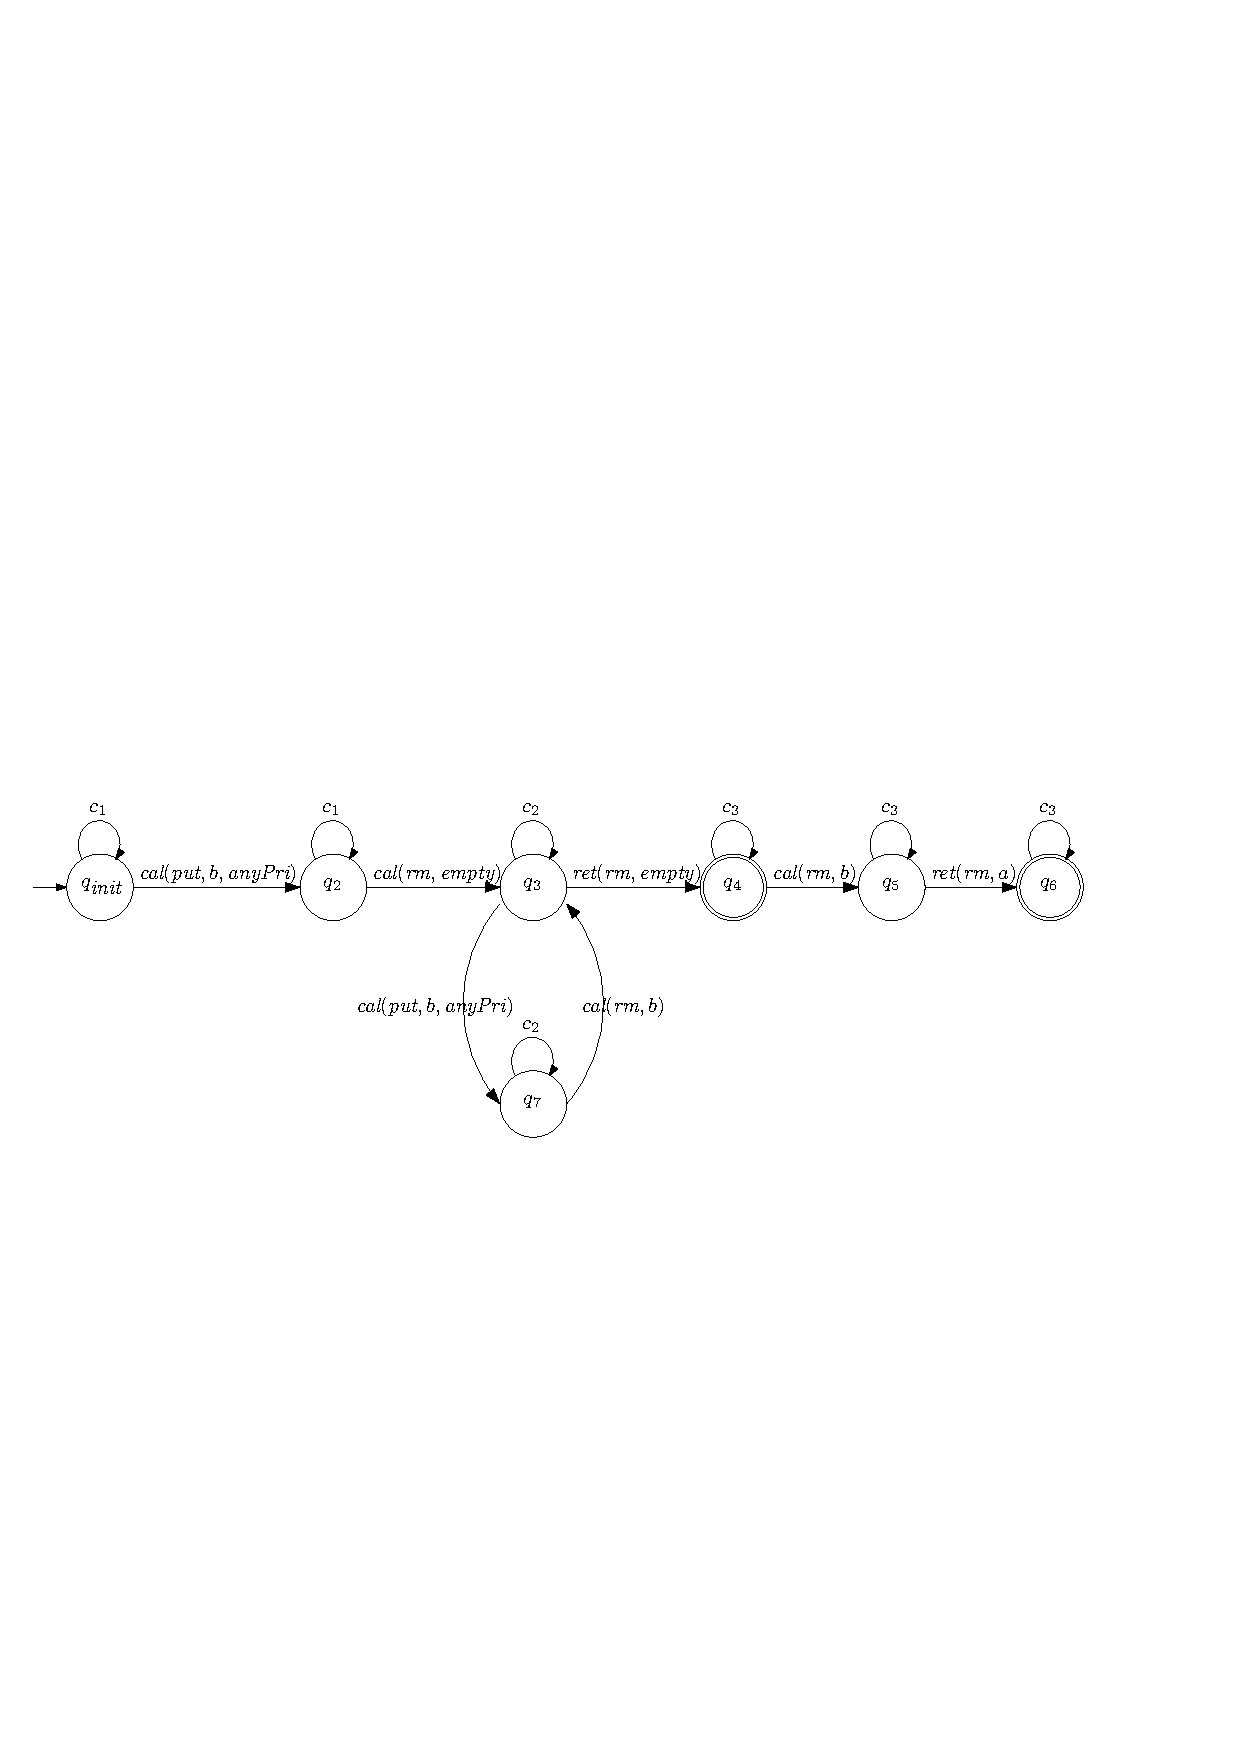
\includegraphics[width=0.8 \textwidth]{PIC_AUTO_Rpr5.pdf}
%\vspace{-10pt}
  \caption{Automaton $\mathcal{A}_{\textit{Rpr5}}$}
  \label{fig:automata for Rpr5}
\end{figure}

Given a data-differentiated history $h$, we say that $o = \textit{rm}(\textit{empty})$ in $h$ is covered by items $d_1,\ldots,d_m$ in $h$, if

\begin{itemize}
\setlength{\itemsep}{0.5pt}
\item[-] $\textit{put}(d_m,\_)$ happens before $o$,

\item[-] For each $i < 1 \leq m$,$\textit{put}(d_{\textit{i-1}},\_)$ happens before $\textit{rm}(d_i)$,

\item[-] $o$ happens before $\textit{rm}(d_1)$, or $\textit{rm}(d_1)$ does not exists in $h$
\end{itemize}

According to the definition of left-right constraint for $o$, in a data-differentiated history $h$, there is a cycle going through $o$, if and only if there exists items $d_1,\ldots,d_m$, such that $o$ is covered by $d_1,\ldots,d_m$.


\begin{restatable}{lemma}{Rpr5IsCoRegular}
\label{lemma:Rpr1 5s co-regular}
$R_{\textit{pr5}}$ is co-regular.
\end{restatable}

\begin {proof}

We need to prove that:

\noindent {\bf $\textit{fact}_1$}: Given a data-independent implementation $\mathcal{I}$, $\mathcal{A}_{\textit{Rpr5}} \cap \mathcal{I} \neq \emptyset$, if and only if there exists data-differentiated history $h \in \mathcal{I}$, $h'$ is a projection of $h$, $\textit{last}(h') = R_{\textit{pr5}}$ and $h$ does not linearizable to $\textit{MR}_{\textit{pr5}}$.

By Lemma \ref{lemma:Gap Equals Lin for Rpr5} and Lemma \ref{lemma:Gap Equals Constraint for Rpr5}, $\textit{fact}_1$ is equivalent to $\textit{fact}_2$:

\noindent {\bf $\textit{fact}_2$}: Given a data-independent implementation $\mathcal{I}$, $\mathcal{A}_{\textit{Rpr5}} \cap \mathcal{I} \neq \emptyset$, if and only if there exists data-differentiated history $h \in \mathcal{I}$, $h''$ is a projection of $h$, such that $\textit{last}(h'') = R_{\textit{pr5}}$, $o = \textit{rm}(\textit{empty})$ is in $h''$, and $o$ is covered by some items $d_1,\ldots,d_m$ in $h''$.


\noindent The $\textit{only if}$ direction: Assume that $h_1 \in \mathcal{I}$ is accepted by $\mathcal{A}_{\textit{Rpr5}}$. By data-independence, there exists data-differentiated sequence $h_2 \in \mathcal{I}$ and a renaming function $r$, such that $h_1=r(h_2)$. Let $d_1,\ldots,d_m$ be the items in $h_2$ such that $r(d_i)=d$ for each $1 \leq i \leq m$. Let $h'' = h_2 \vert_{ \{ o, d_0, d_1, \ldots, d_m \} }$. It is obvious that $\textit{last}(h'') = R_{\textit{pr5}}$. It is easy to see that $o$ is covered by $d_1,\ldots,d_m$.

\noindent The $\textit{if}$ direction: Assume that there exists such $h$, $h''$, $o$ and $d_1,\ldots,d_m$. Then, let $h_1$ be obtained from $h$ by renaming $d_1,\ldots,d_m$ into $b$ and renaming other items into $d$. We can prove that $h_1$ is accepted by $\mathcal{A}_{\textit{Rpr5}}$.

This completes the proof of this lemma. \qed
\end {proof}




\section{Relate Queue and Stack with Priority Queue}
\label{sec:relate queue and stack with priority queue}




\subsection{Relate Queue with Priority Queue}
\label{subsec:relate queue with priority queue}

Given a history $h_q$ of queue operations, let $\textit{UniPriTrans}(h_q)$ be a history of priority queue, which is generated as follows: transform each $\textit{call}(\textit{enq},a)$, $\textit{ret}(\textit{enq},a)$, $\textit{call}(\textit{deq},a)$ and $\textit{ret}(\textit{deq},a)$ of $h_q$ into $\textit{call}(\textit{put},a,1)$, $\textit{ret}(\textit{put},a)$, $\textit{call}(\textit{rm},a)$ and $\textit{ret}(\textit{rm},a)$.

\begin{restatable}{lemma}{RelateQueuewithPQ}
\label{lemma:relate queue with priority queue}
Given a history $h_q$ of queue operations, $h_q$ is linearizable to queue, if and only if $\textit{UniPriTrans}(h_q) \sqsubseteq \textit{PQueue}$.
\end{restatable}

\begin {proof}

This is obvious, since we already ensure that for each single-priority history $h$, $\textit{transToQueue}(h)$ is linearizable to queue. \qed
\end {proof}









\end{document}








